\chapter{Simulation Results}

This chapter aims to analyze and compare the accuracy and the performance of all formulations. Most simulations were run on a domain with 101 fault elements, or 303 fault nodes, over a period of 250 years such that one earthquake happens in the considered time frame. Because of the convergence issues of the compact DAE, a full simulation cannot be performed and it was omitted in most discussions. After a rough comparison of the physical simulation results in \autoref{sec:Results_EvolutionSlipRate}, the accuracy for varying tolerances is investigated in \autoref{sec:Results_AccuracyTimeIntegration} and an in-depth accuracy discussion of the second order ODE formulation is conducted in \autoref{sec:Results_ErrorEstimate2ndOrderODE}. The impact of the BDF order on the number of timesteps for implicit methods is discussed in \autoref{sec:Results_BDFOrder} and finally, the scalability of several performance metrics, with a direct comparison between all formulations, is presented in \autoref{sec:Results_Scalability}.

\section{Evolution of physical quantities}
\label{sec:Results_EvolutionSlipRate}
The simulation is run over a period of 250 years, in which one earthquake occurs on June 13th of the 195th year. This event can be clearly observed in \autoref{fig:timeEvolutionTANDEM_V} which depicts the maximum slip rate over time and reaches at its high $4.6m\cdot s^{-1}$ as opposed to an average of $1.0 \cdot 10^{-9}m\cdot s^{-1}$ in calm times. 
\begin{figure}[H]
    \centering
    \begin{subfigure}[b]{0.45\textwidth}
     	\centering
    	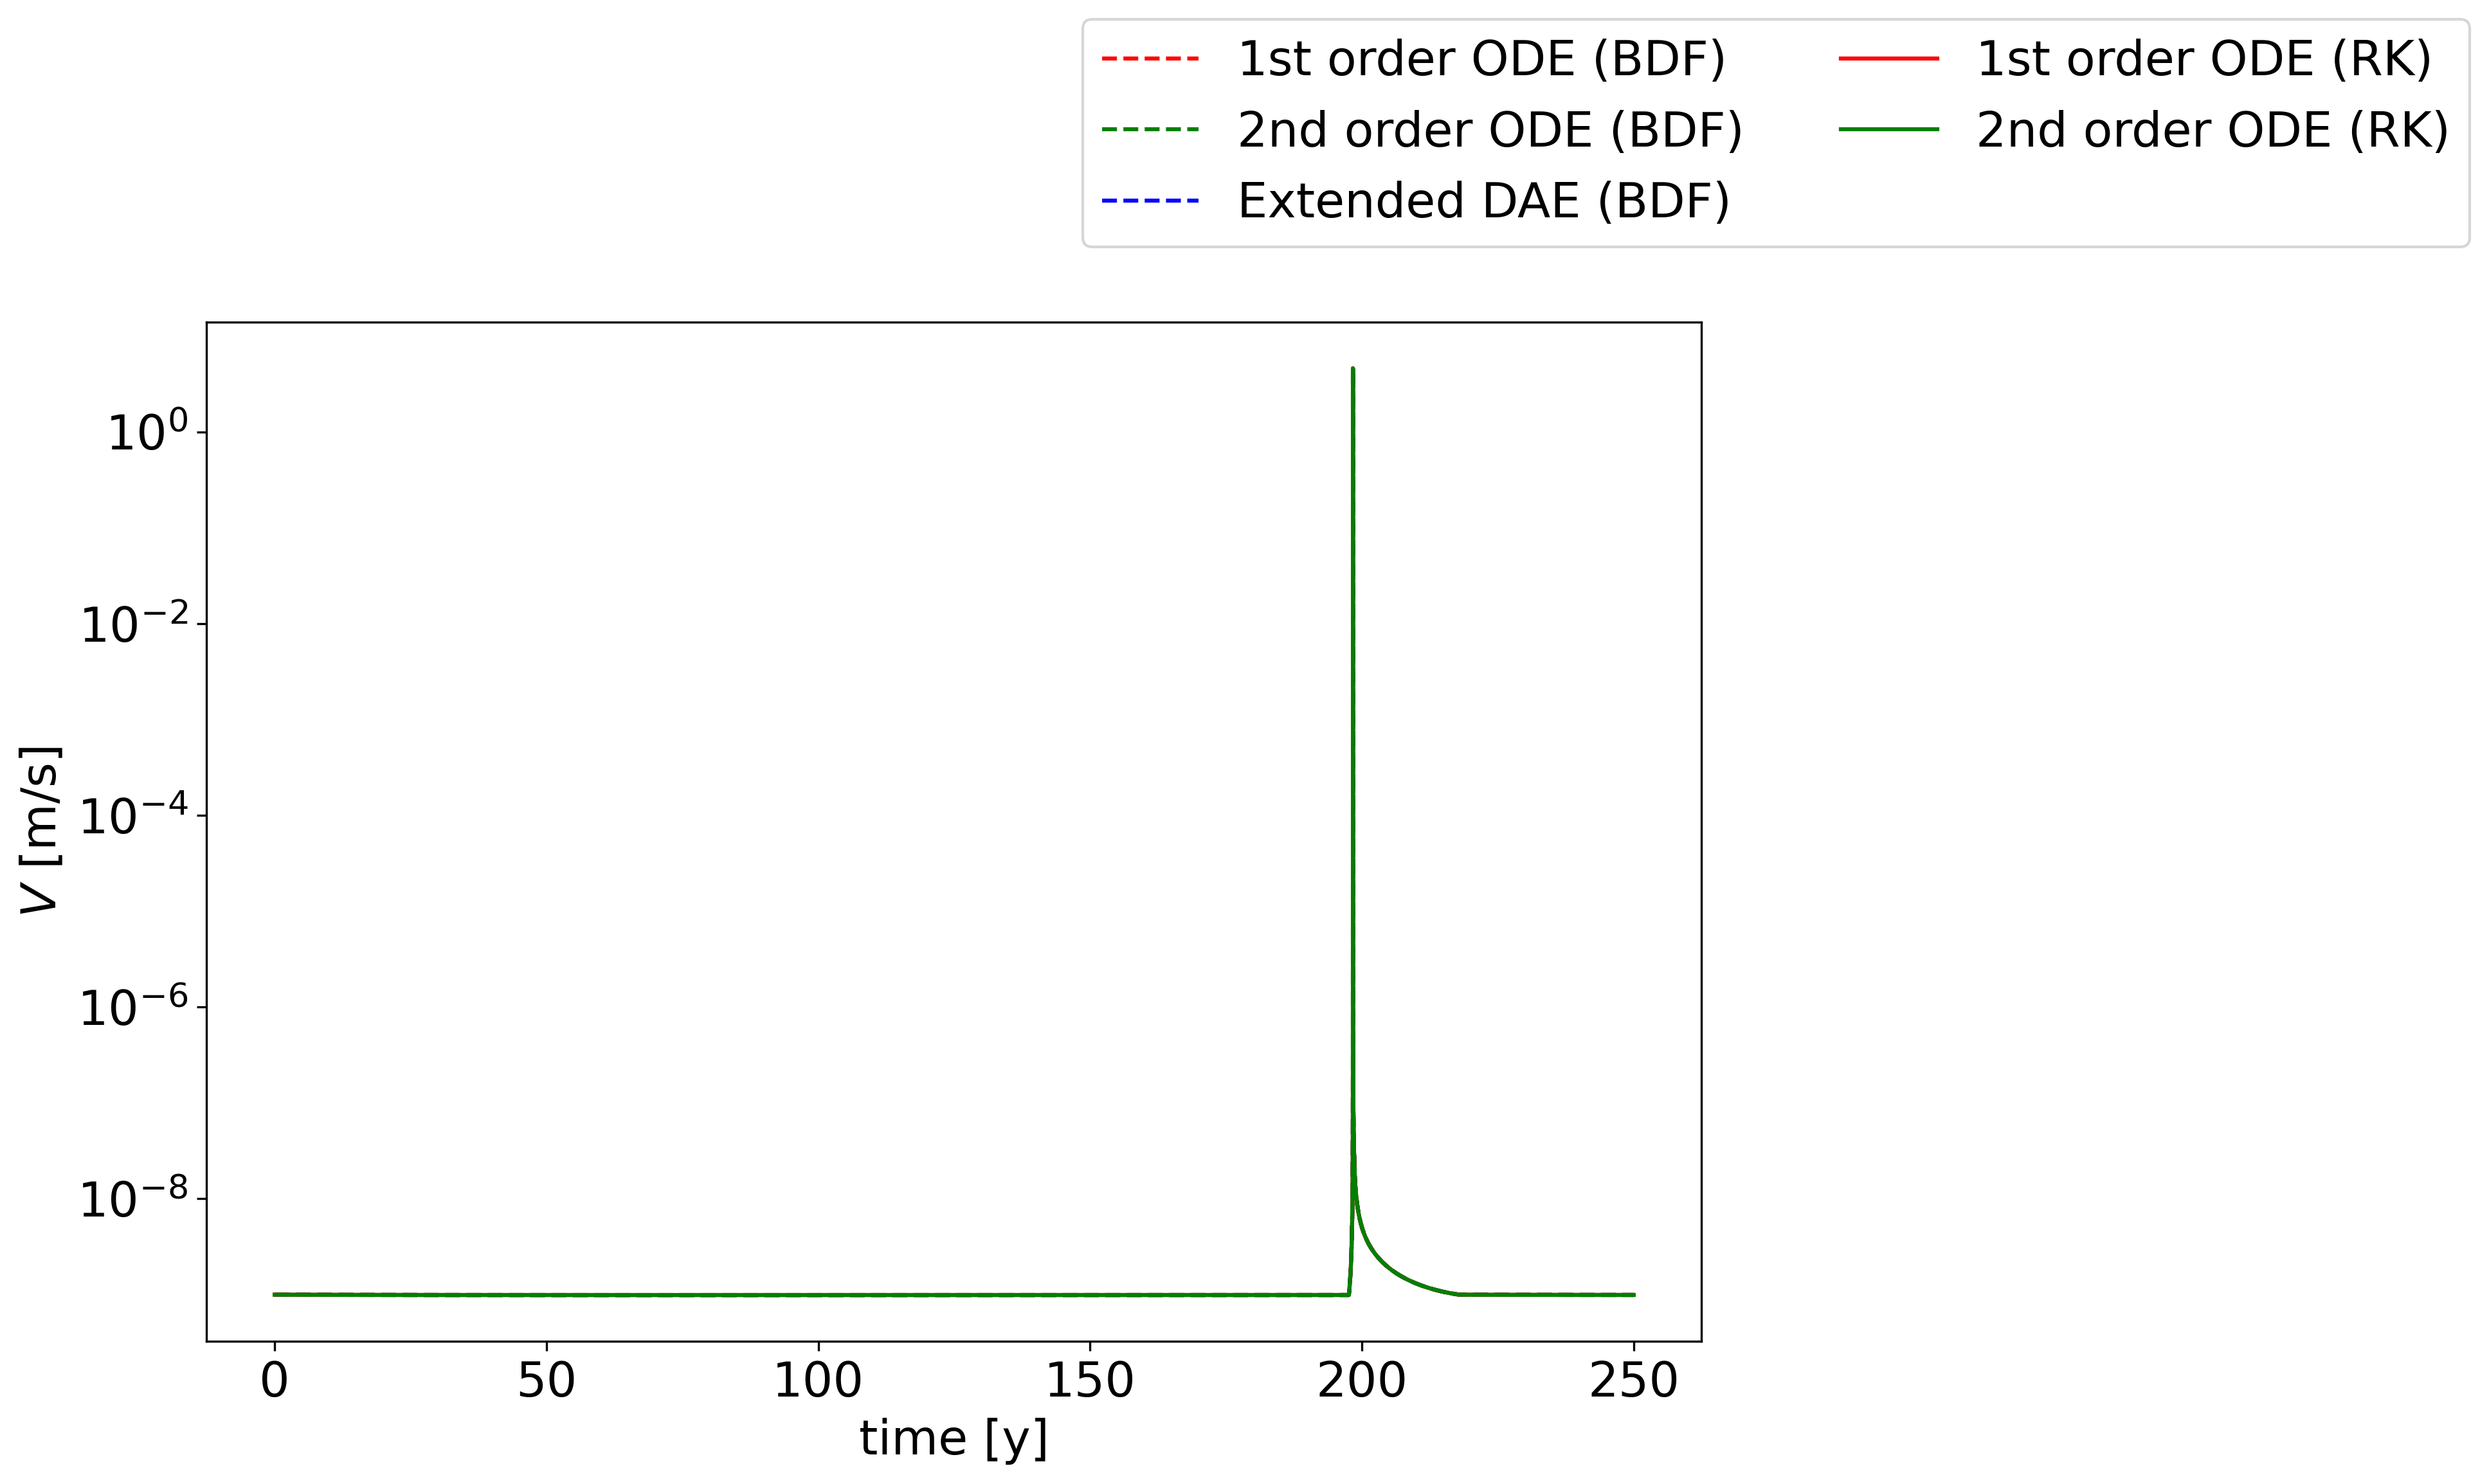
\includegraphics[width=1.45\textwidth]{images/TANDEMtimeEvolution_2D_maxSlipRate_allFormulations.png}
       	\subcaption{Full simulation time} 
    \end{subfigure} 
    \begin{subfigure}[b]{0.45\textwidth}
    	\centering
    	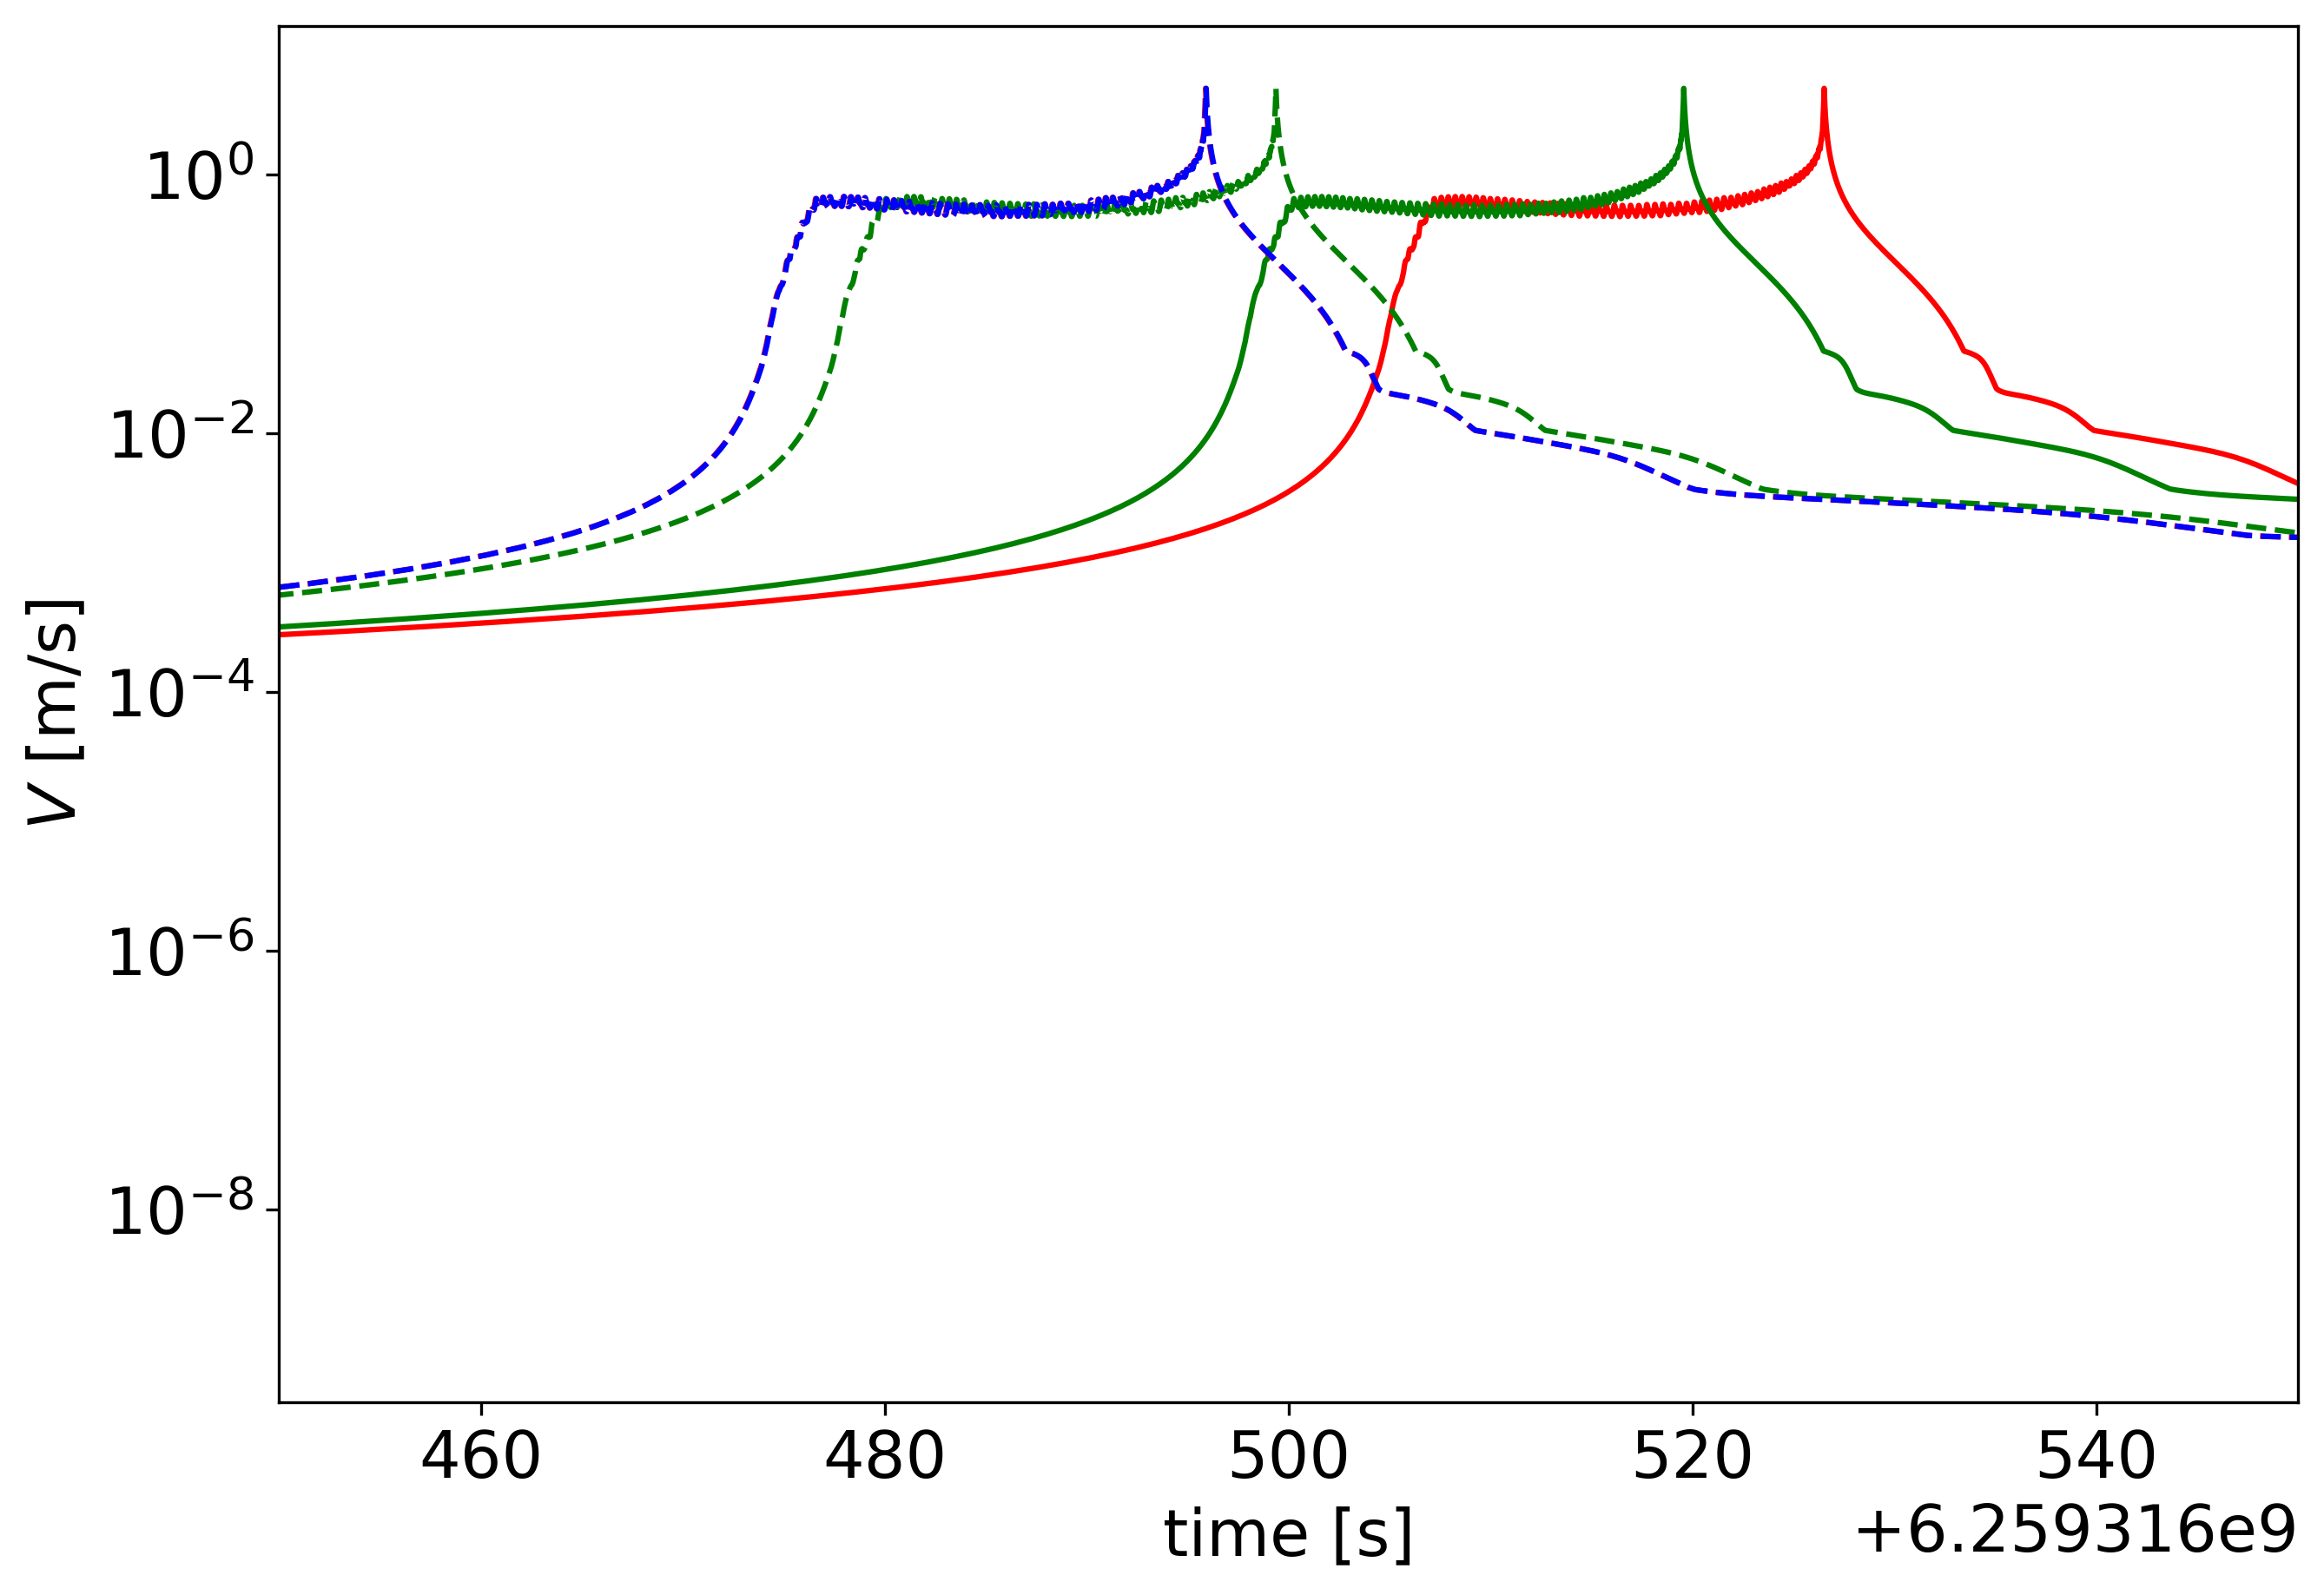
\includegraphics[width=1\textwidth]{images/TANDEMtimeEvolution_2D_maxSlipRate_allFormulations_Earthquake.png}
       	\subcaption{Zoom onto the earthquake event} 
    \end{subfigure}
    \caption{Evolution of the maximal slip rate $V$ on the fault for different solvers on the symmetric two-dimensional BP1 problem with 200 fault elements}
    \label{fig:timeEvolutionTANDEM_V}
\end{figure}
Looking at the evolution over the whole simulation time, no difference between the formulations can be spotted. Only a very close look at the seconds surrounding the main earthquake peak gives a hint that the results from the different formulations do not perfectly match. The shape of the curves is the same, but they occur with a time delay of up to 40 seconds, more than the duration of the earthquake itself. Considering that the earthquake happens after almost 200 years, a time difference of 40 seconds is actually neglectable and it can be stated that all formulations return the same results with high accuracy. This time shift stems rather from the preceding aseismic phase than from the earthquake phase, as the qualitative evolution within the rupture event is identical. It seems that implicit methods predict earthquakes earlier than explicit ones, and the results of the implicit 1st order ODE and extended DAE formulations overlap so well that their respective curves cannot be distinguished on the zoomed graph.  \\
The same conclusion could also be drawn with the evolution of the slip or the state variable, who perfectly match each other unless one zooms onto the seconds surrounding the earthquake event. 


\section{Accuracy of the time integration}
\label{sec:Results_AccuracyTimeIntegration}
The discussion in \autoref{ssec:LowerBoundTimeTolerance} only tackled the question of the lowest allowable tolerances to reach as accurate results as possible. However, such strict tolerances may severely reduce the timestep size and by consequence the length of the simulation. For many applications, satisfactory results are already obtained for larger tolerances, and the aim of this section is to investigate it for SEAS. As there is no mathematical definition for \textit{satisfactory results} (unless convergence is the only requirement), we will run the simulation with the strictest possible tolerance described in the previous section and assess how the results deteriorate as the tolerances increase. Tolerances can be defined independently for the 
aseismic slip and for the earthquake, and will therefore be investigated separately. \\

The first set of experiments is performed with the 1st order ODE formulation on a domain with 101 fault elements to characterize the aseismic slip. The reference solution corresponds to the absolute tolerances $t_a^S =10^{-11}$ and $t_a^\psi =10^{-13}$, and this tolerance is kept in the earthquake phase for all simulation runs. In the simulated time of 300 years, two earthquakes occur after 204 and 270 years, and the accuracy is measured with the occurrence time of the first earthquake and with the period between the two events. The exact times are defined as the moment of the timestep, in which the highest maximum slip rate is reached. These metrics are appropriate, because the fundamental task of the aseismic slip is to build up stress until an earthquake is triggered, and an accurate simulation environment should detect the same earthquakes at the same times. The results are collected in \autoref{fig:tolerancesAseismicSlip_compactODE} for both the explicit, 5th order, Dormand-Prince RK method and the implicit, adaptive-order, BDF scheme.
\begin{figure}[H]
	\centering
	\begin{subfigure}[t]{0.32\textwidth}
		\centering
		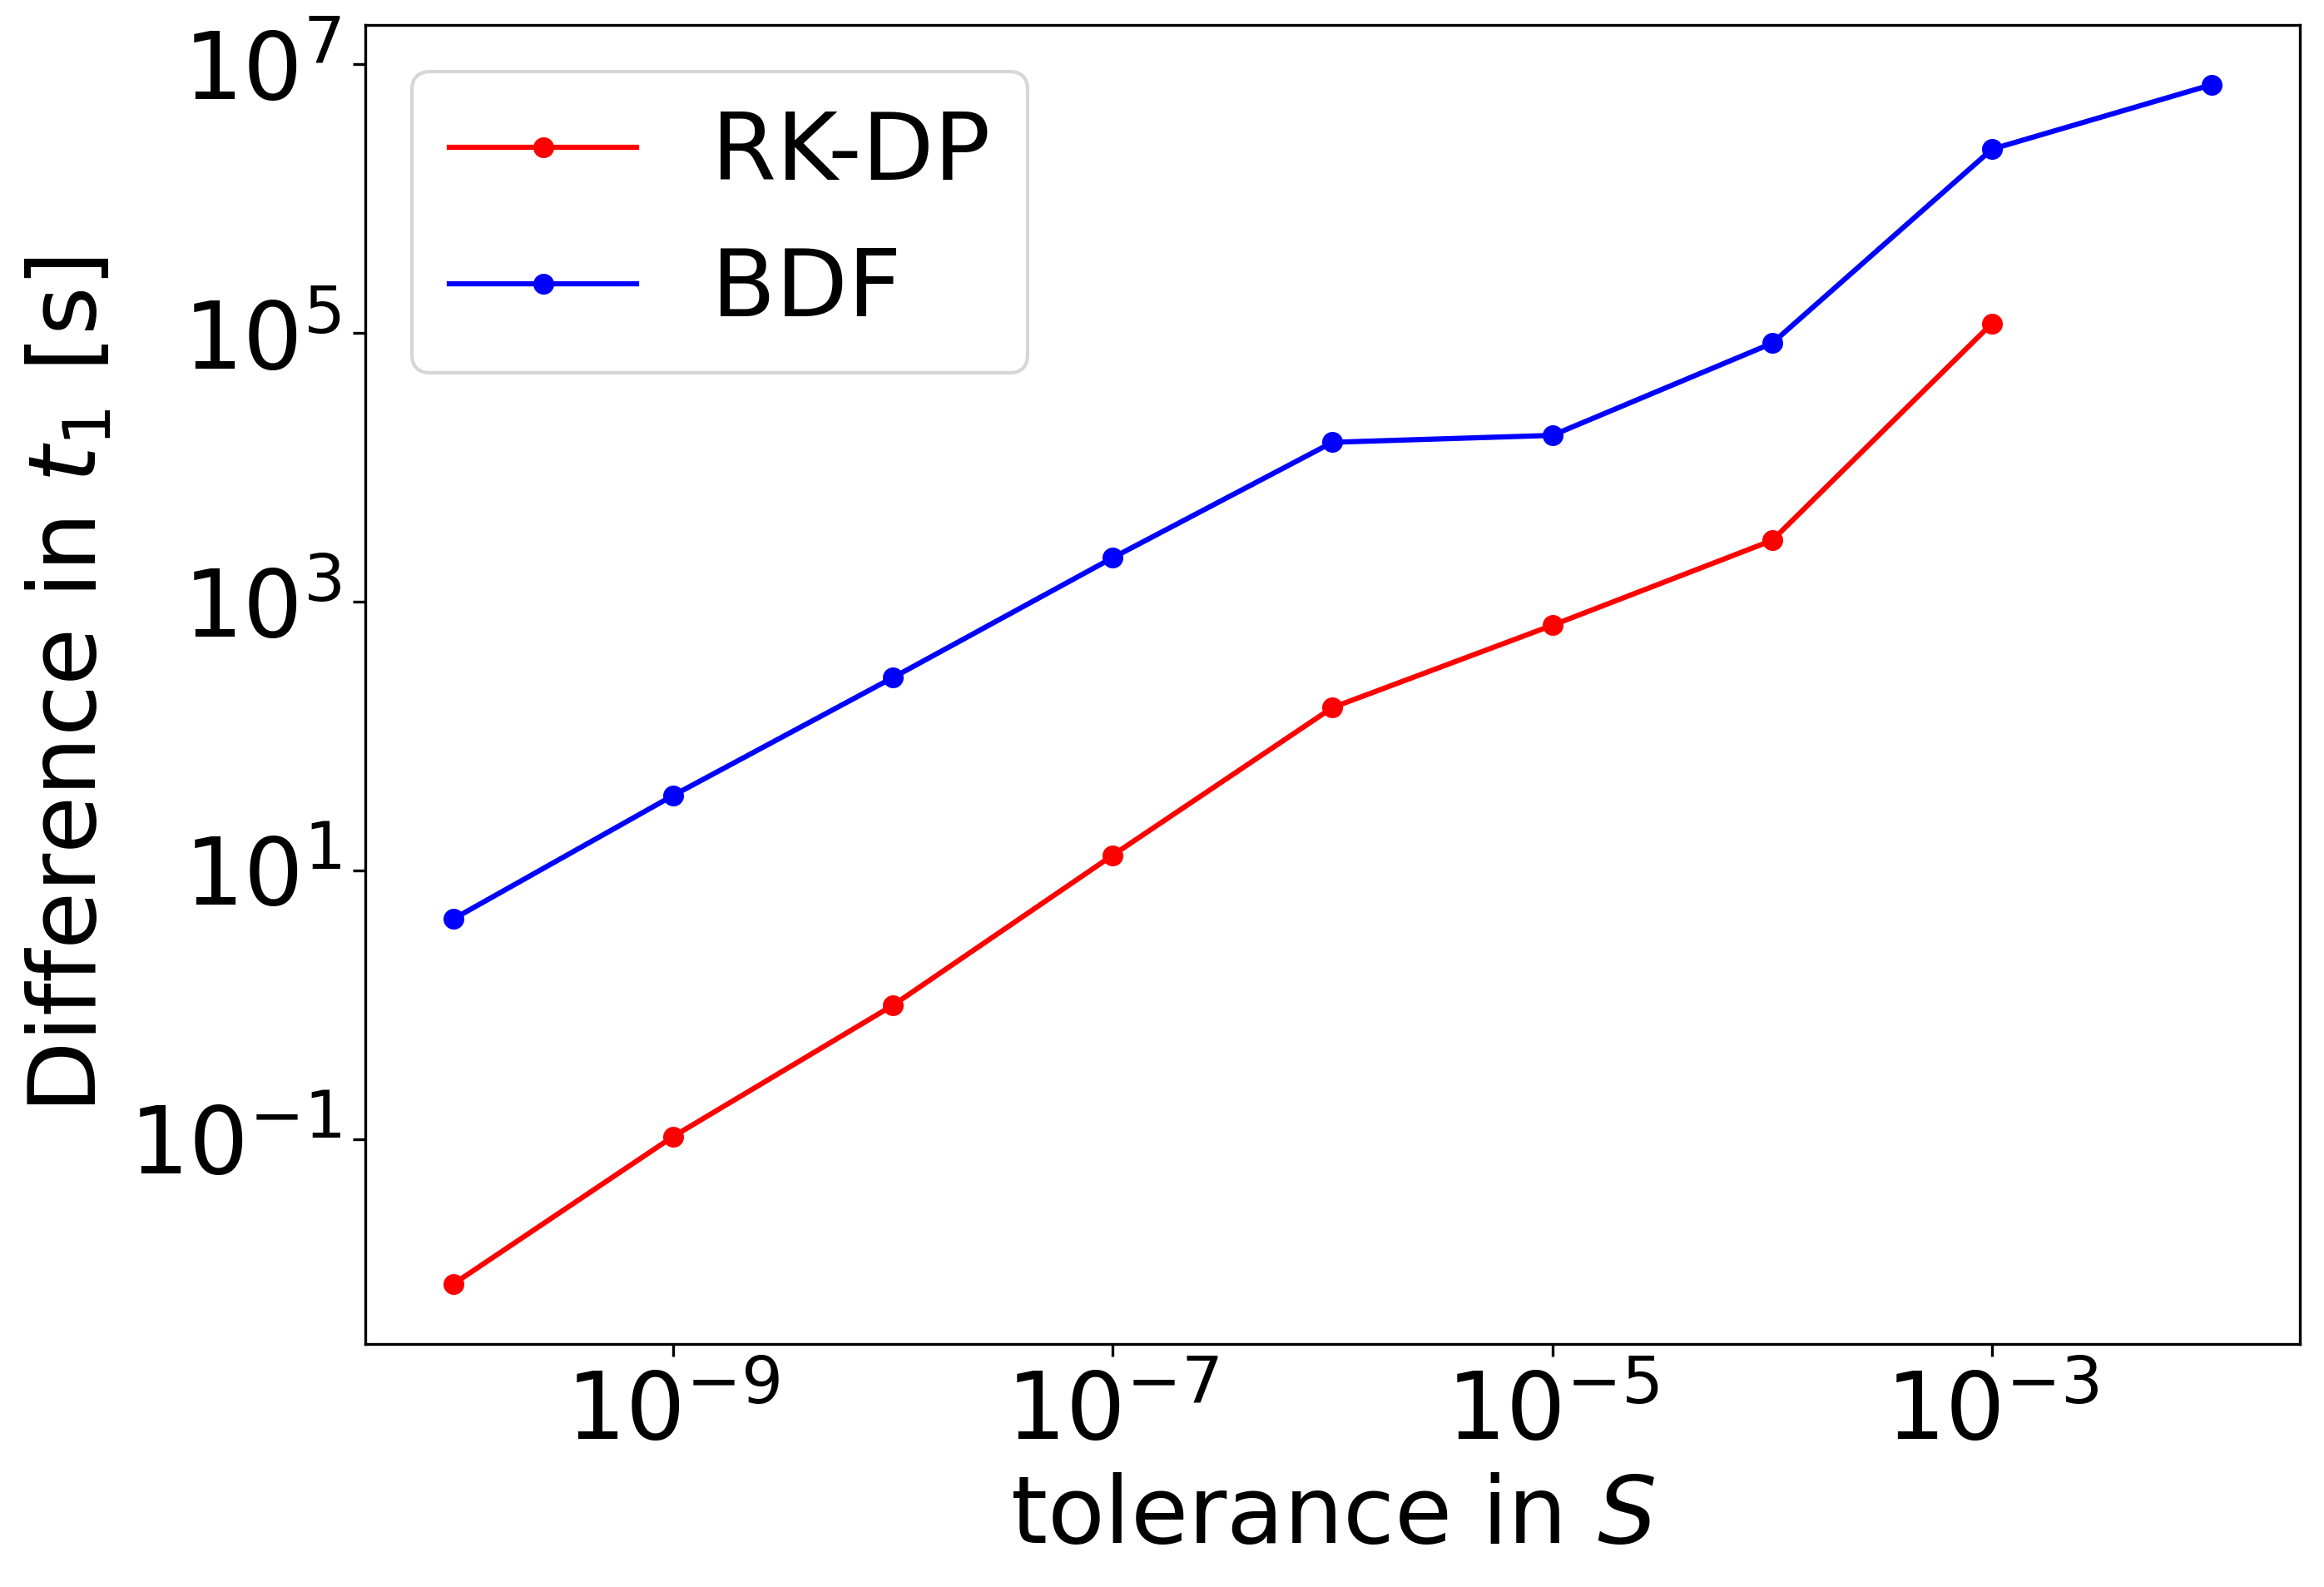
\includegraphics[width=1\textwidth]{images/TANDEMcompactODEDifferentTolerancesSize101_AS_FirstEarthquakeTimeDiff.png}
		\subcaption{Time difference of the first earthquake} 
	\end{subfigure} 
	\begin{subfigure}[t]{0.32\textwidth}
		\centering
		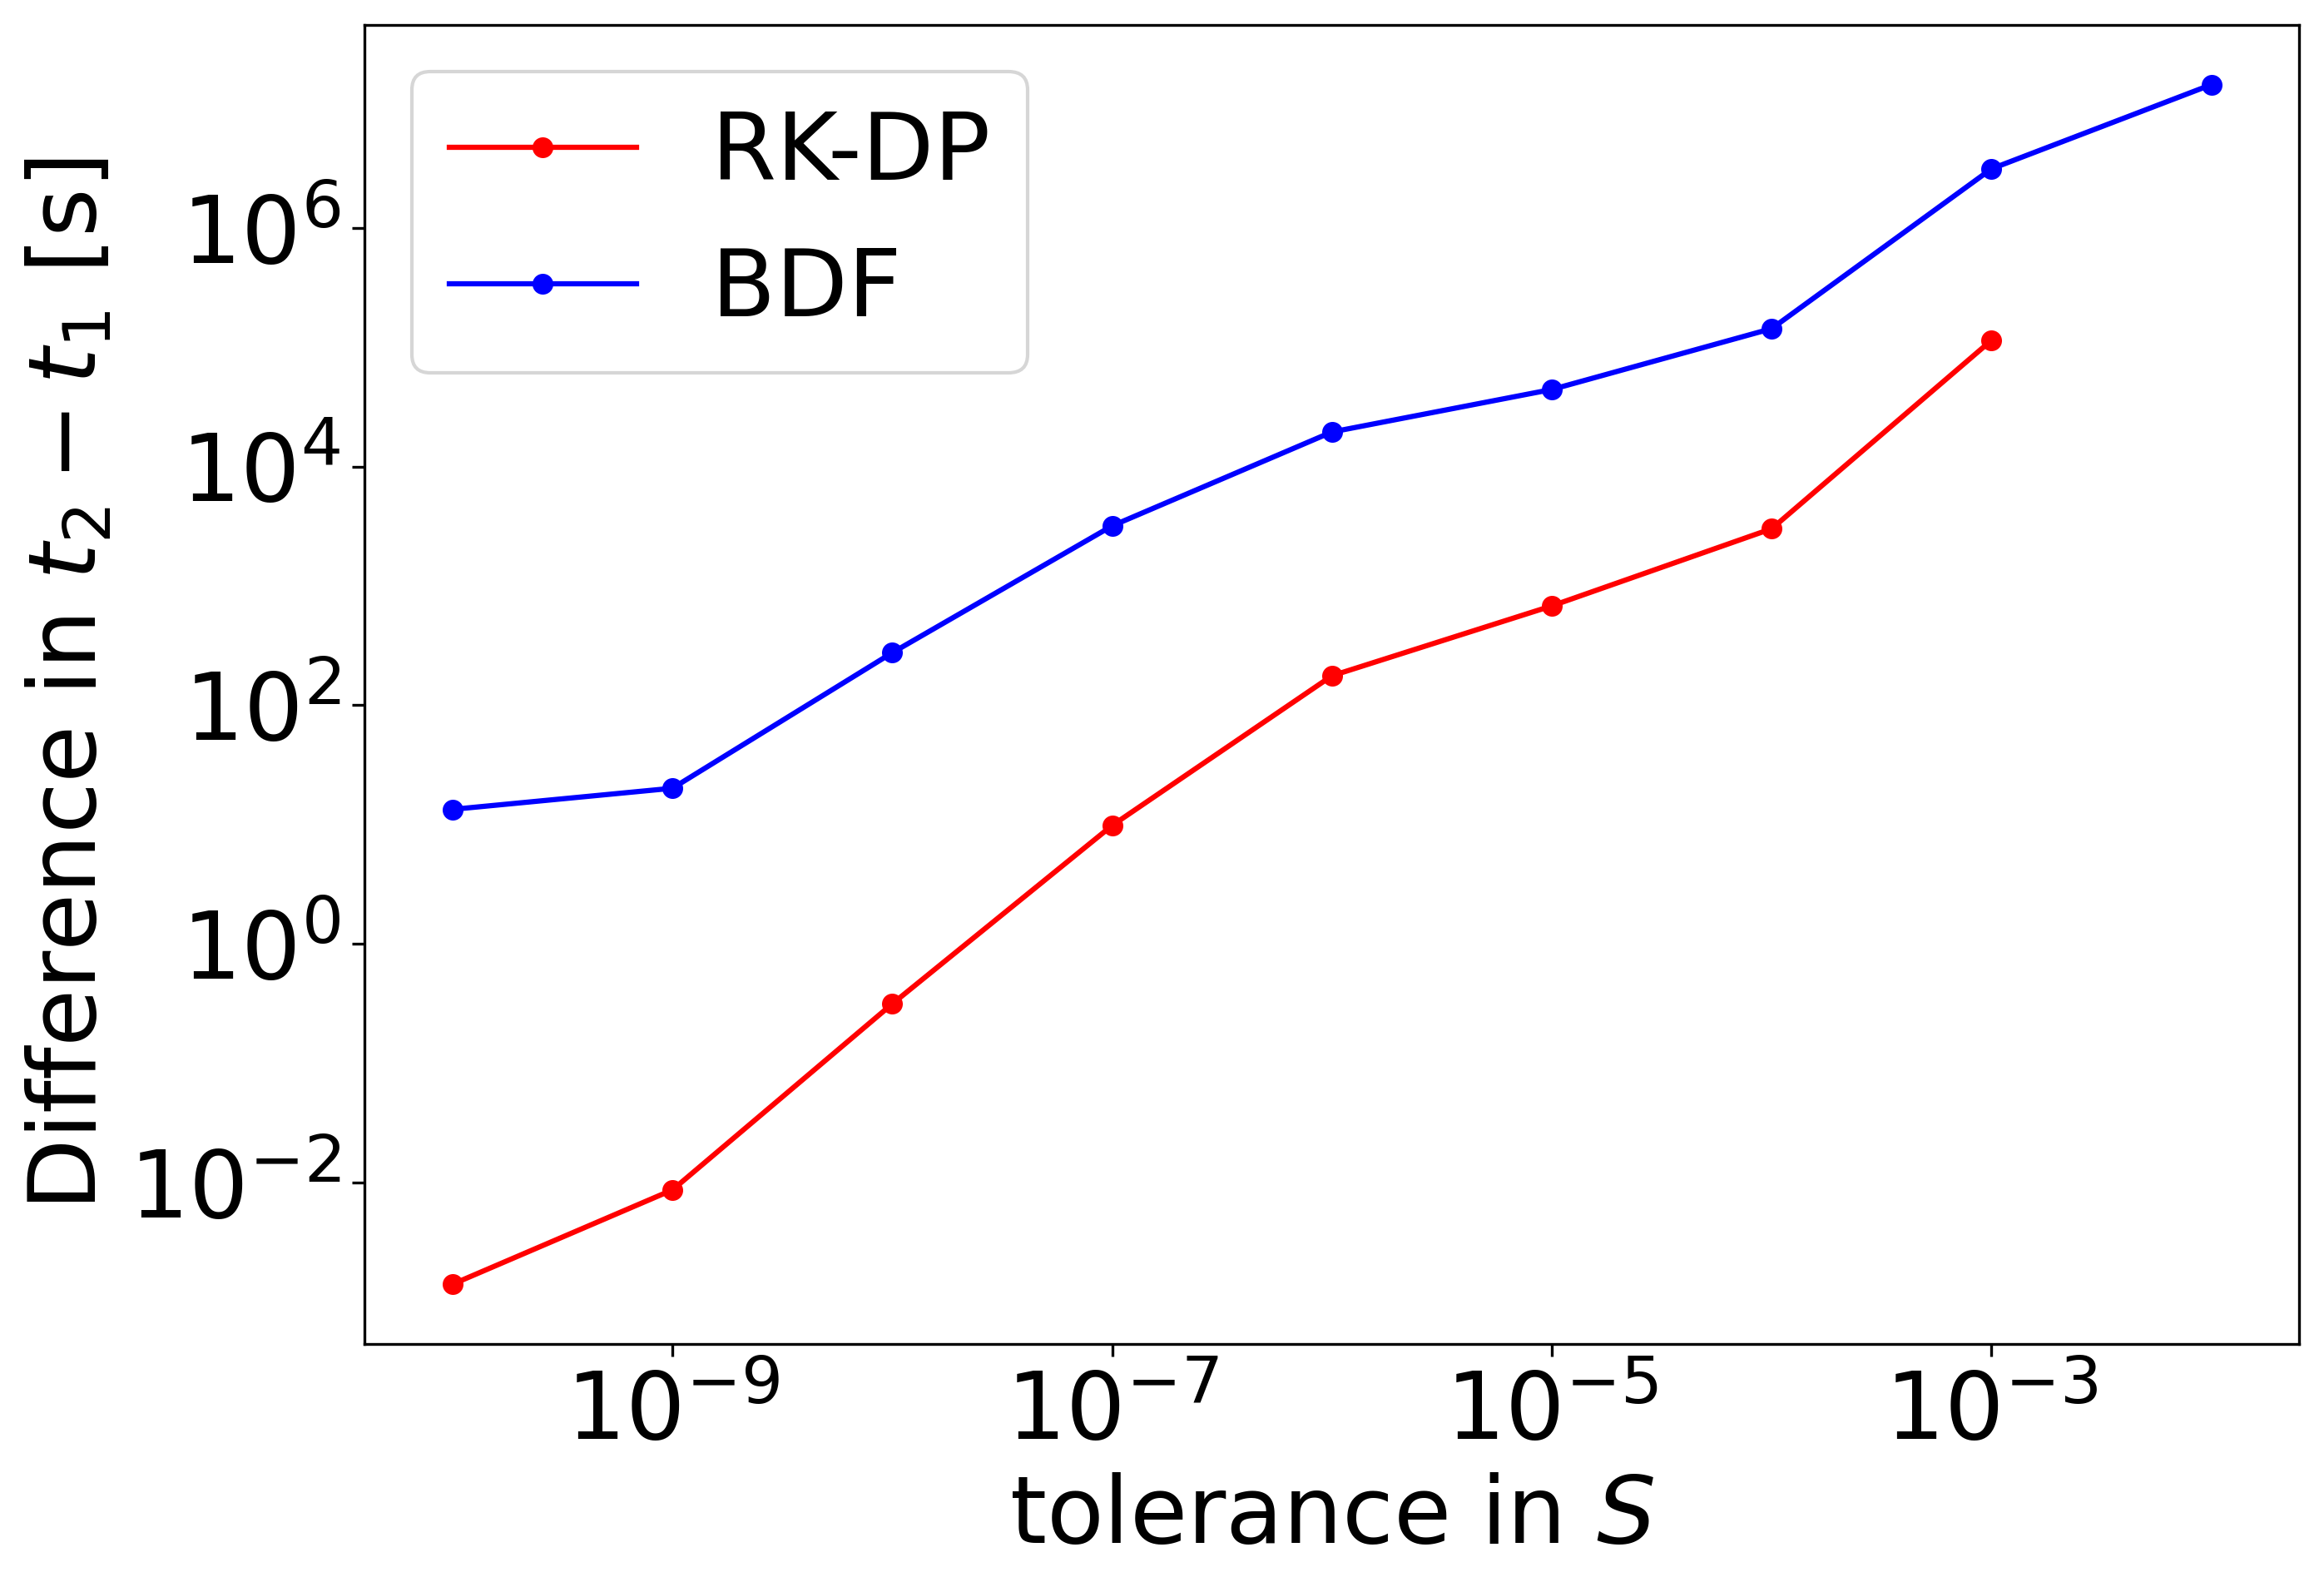
\includegraphics[width=1\textwidth]{images/TANDEMcompactODEDifferentTolerancesSize101_AS_PeriodDiff.png}
		\subcaption{Difference of the period between both earthquakes} 
	\end{subfigure}
	\begin{subfigure}[t]{0.32\textwidth}
		\centering
		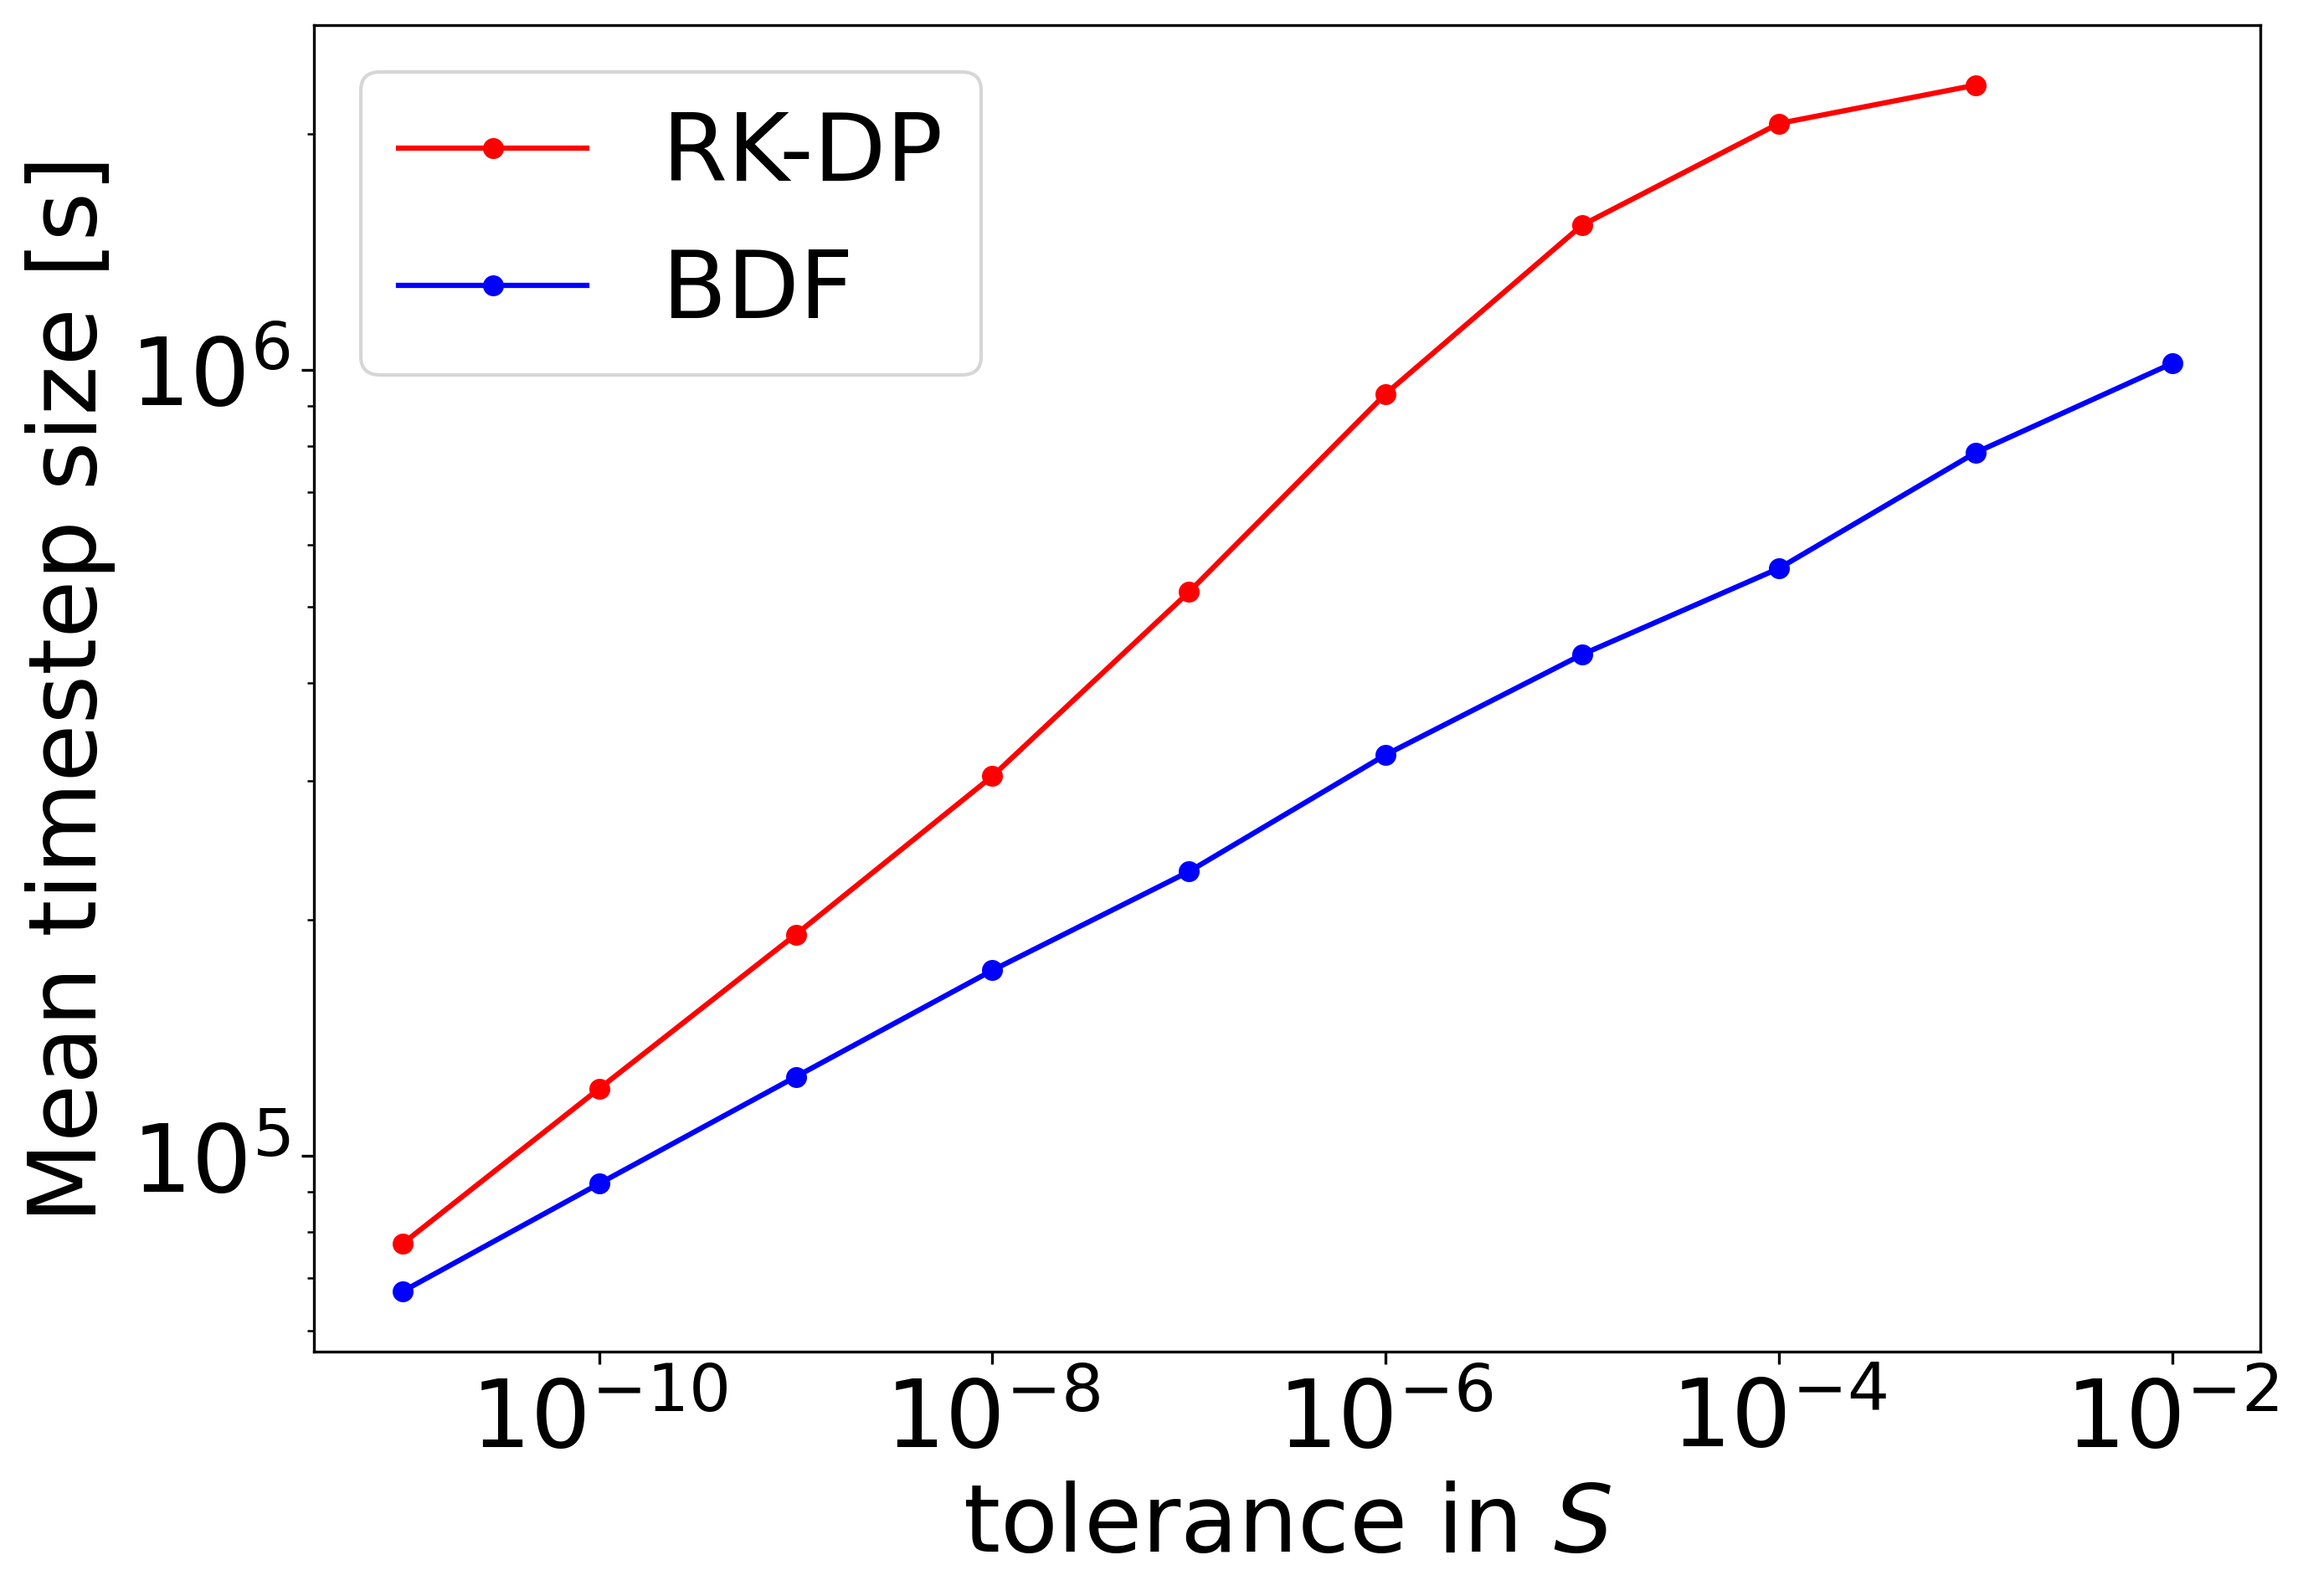
\includegraphics[width=1\textwidth]{images/TANDEMcompactODEDifferentTolerancesSize101_AS_DT.png}
		\subcaption{Geometric mean of the timestep size in the aseismic slip} 
	\end{subfigure}
	\caption{Difference of characteristic times to the reference solution for different tolerances in the aseismic slip phase for a domain with 101 fault elements with the 1st order ODE formulation}
	\label{fig:tolerancesAseismicSlip_compactODE}
\end{figure}

As expected, the accuracy of the predicted times worsens exponentially if the tolerance increases and the relationship. However, it appears that the implicit method deteriorates faster than the explicit,  With the RK method, all tolerances below $t_a^S<10^{-5}$m  and with BDF all below $t_a^S<10^{-7}$m allow to predict the earthquake up to an hour (=3600s) difference, which is very impressive considering the 200 years simulated time until it happens. It is much more accurate than the error induced by the DG scheme. Remember that in ??????? the earthquake got shifted by ?? years if the number of fault elements is doubled. It appears that the RK method fails if the tolerance exceeds $10^{-3}$m, which is not the case for the BDF method. Indeed, in the last few timesteps before the earthquake is triggered, the built-in iterative solver for the friction returns wrong values for $V$ until NaNs are encountered. In BDF, the residual of the Newton iteration diverges right away with wrong slip rates, and the timestep size is scaled down in time. However, at $t_a^S = 10^{-2}$m, which can only be reached with implicit methods, the times are off by $10^7$s $\approx 116$days and thus too inaccurate. \\

In the second experiment, the tolerance for the aseismic phase is kept constant and tolerances in the earthquake phase is progressively decreased. The simulation time is reduced to 250 years, such that only one earthquake occurs. The first quantity we look at is the overall maximum slip rate, that represents the intensity of the earthquake. Another interesting quantity is the increase in slip at the open surface, because this has a direct influence on the prediction of the subsequent earthquake: if the slip did not increase by much, the earthquake was not complete and the next happens earlier and inversely, if the earth moves too much, the next earthquake will be delayed. It is measured as the difference between the minimum slip at the end and the beginning of the simulation, which lie both in the aseismic phase surrounding the earthquake. The accuracy is thus estimated as a combination of the intensity and the geological changes in the earthquake. The results are found in \autoref{fig:tolerancesEarthquake_compactODE}, for the RK-DP and BDF schemes.

\begin{figure}[H]
	\centering
	\begin{subfigure}[t]{0.32\textwidth}
		\centering
		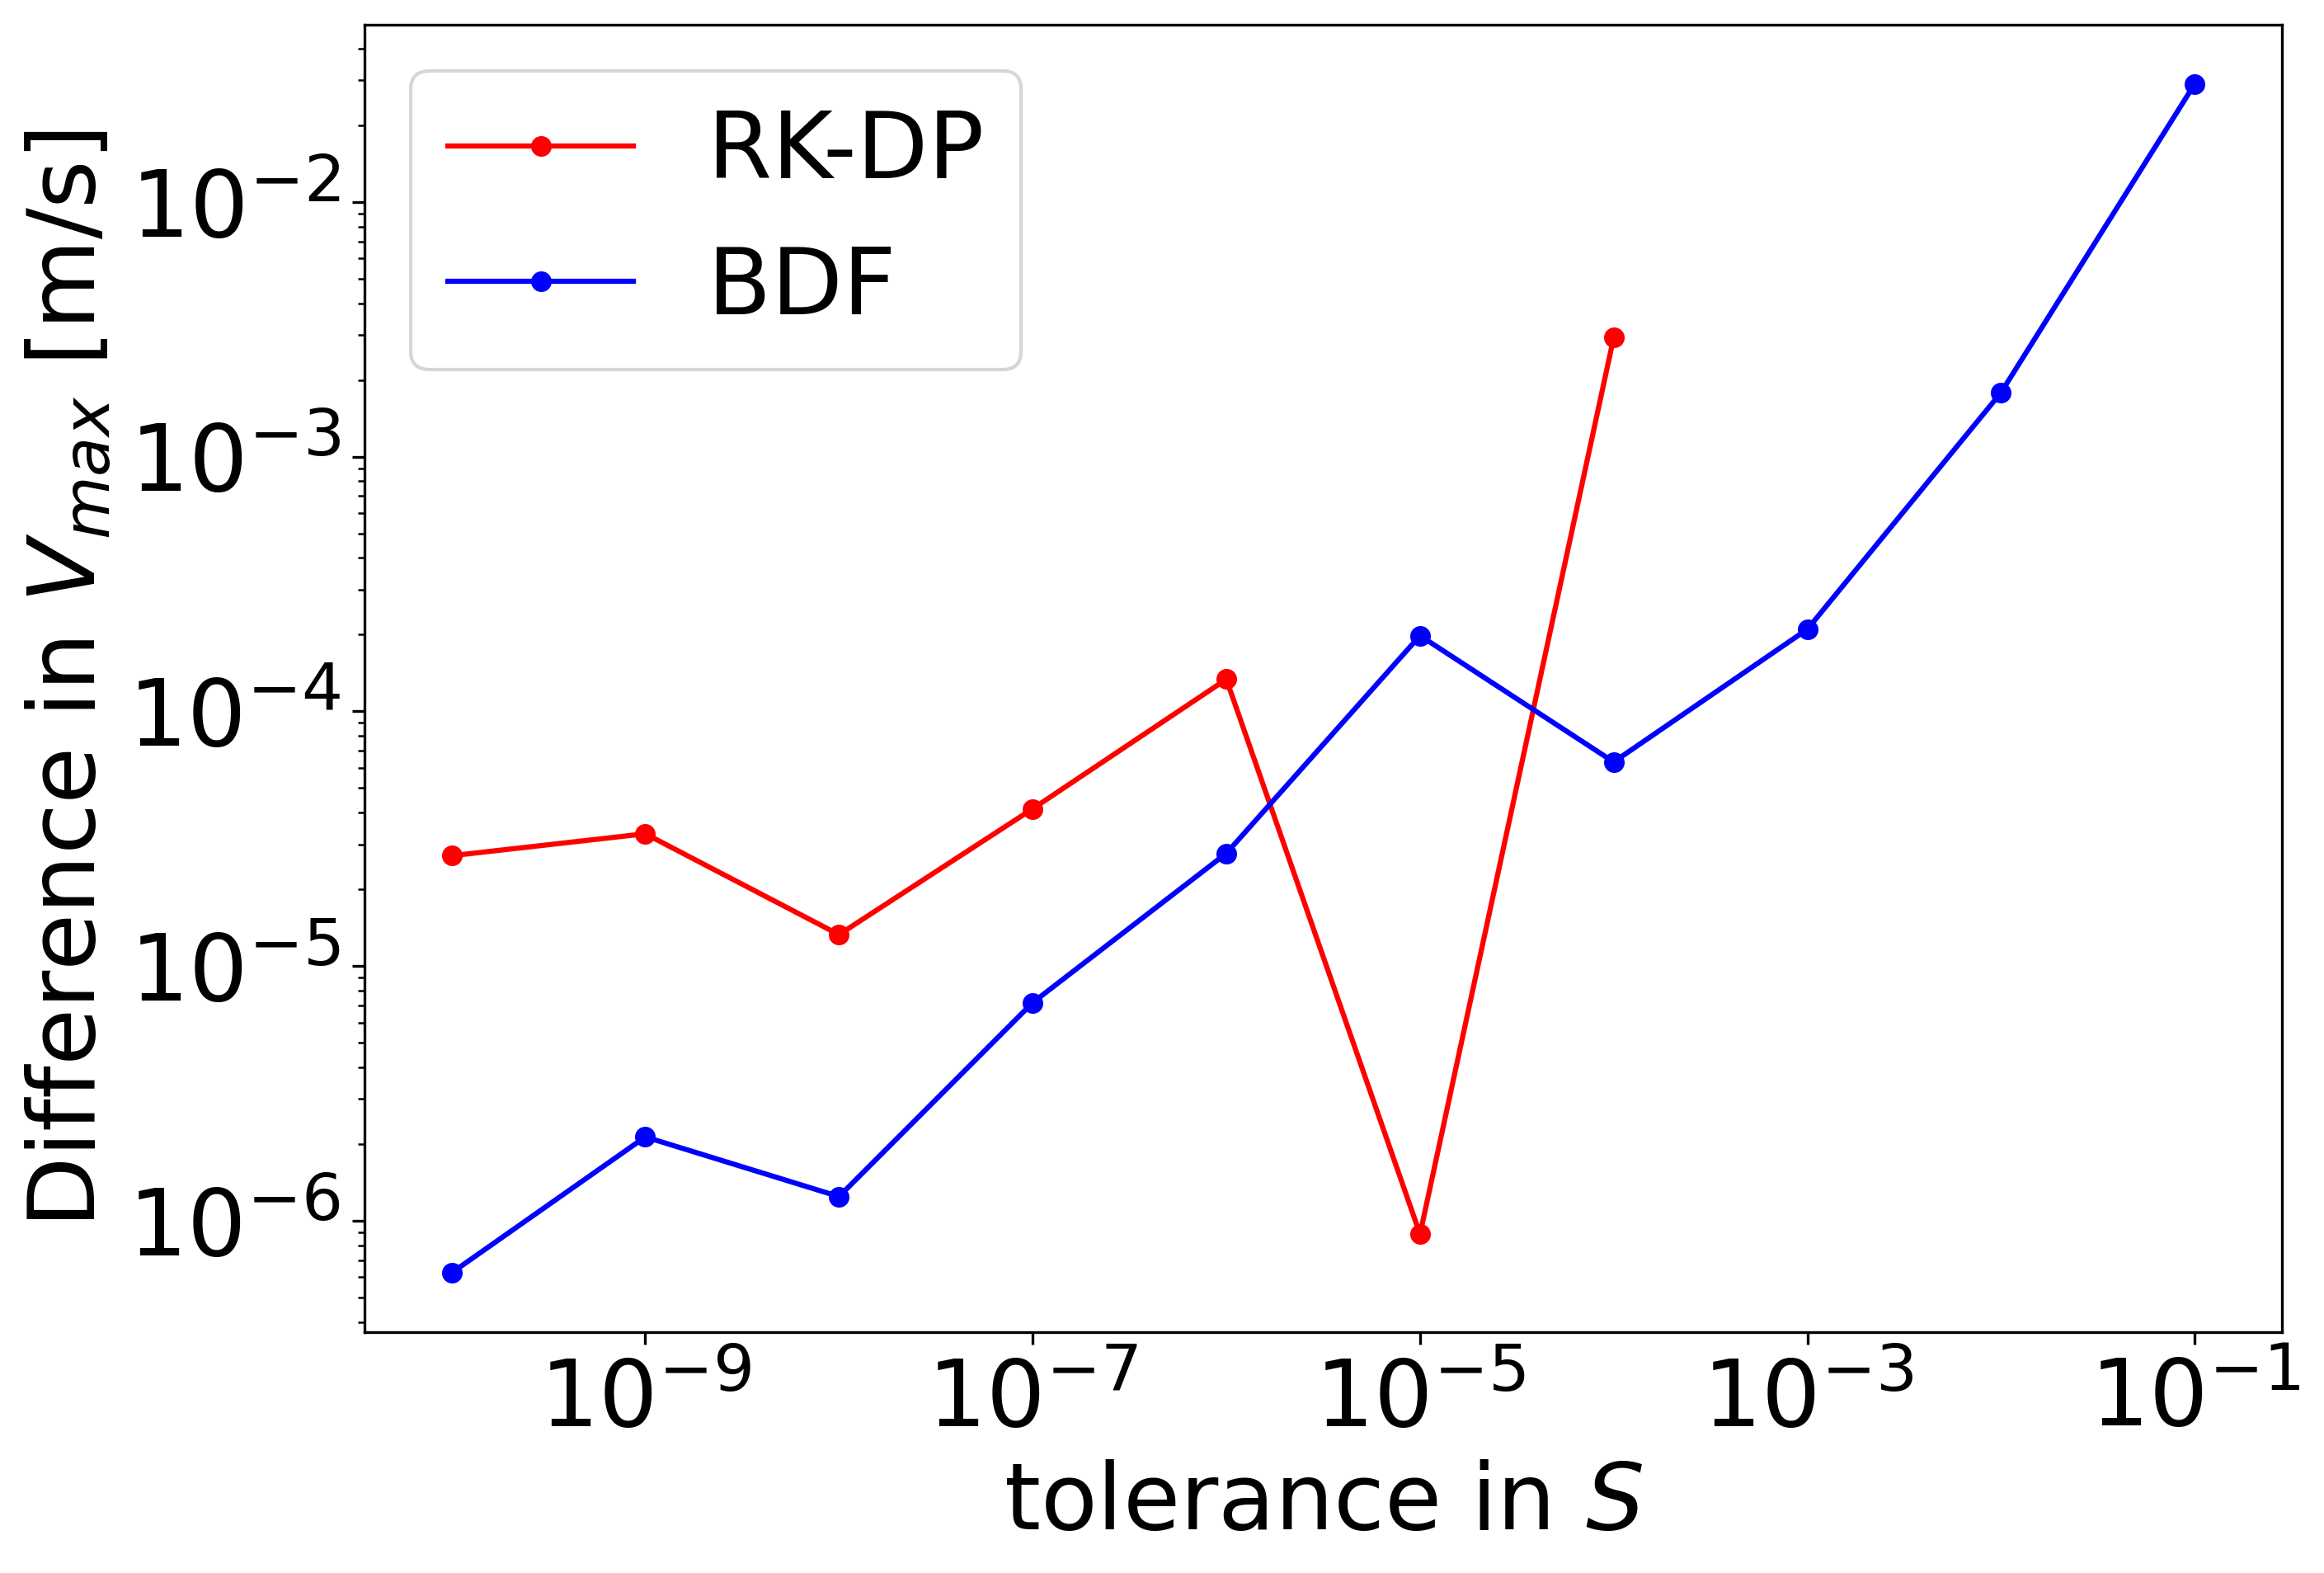
\includegraphics[width=1\textwidth]{images/TANDEMcompactODEDifferentTolerancesSize101_EQ_Vmax.png}
		\subcaption{Difference in the maximum slip rate} 
	\end{subfigure} 
	\begin{subfigure}[t]{0.32\textwidth}
		\centering
		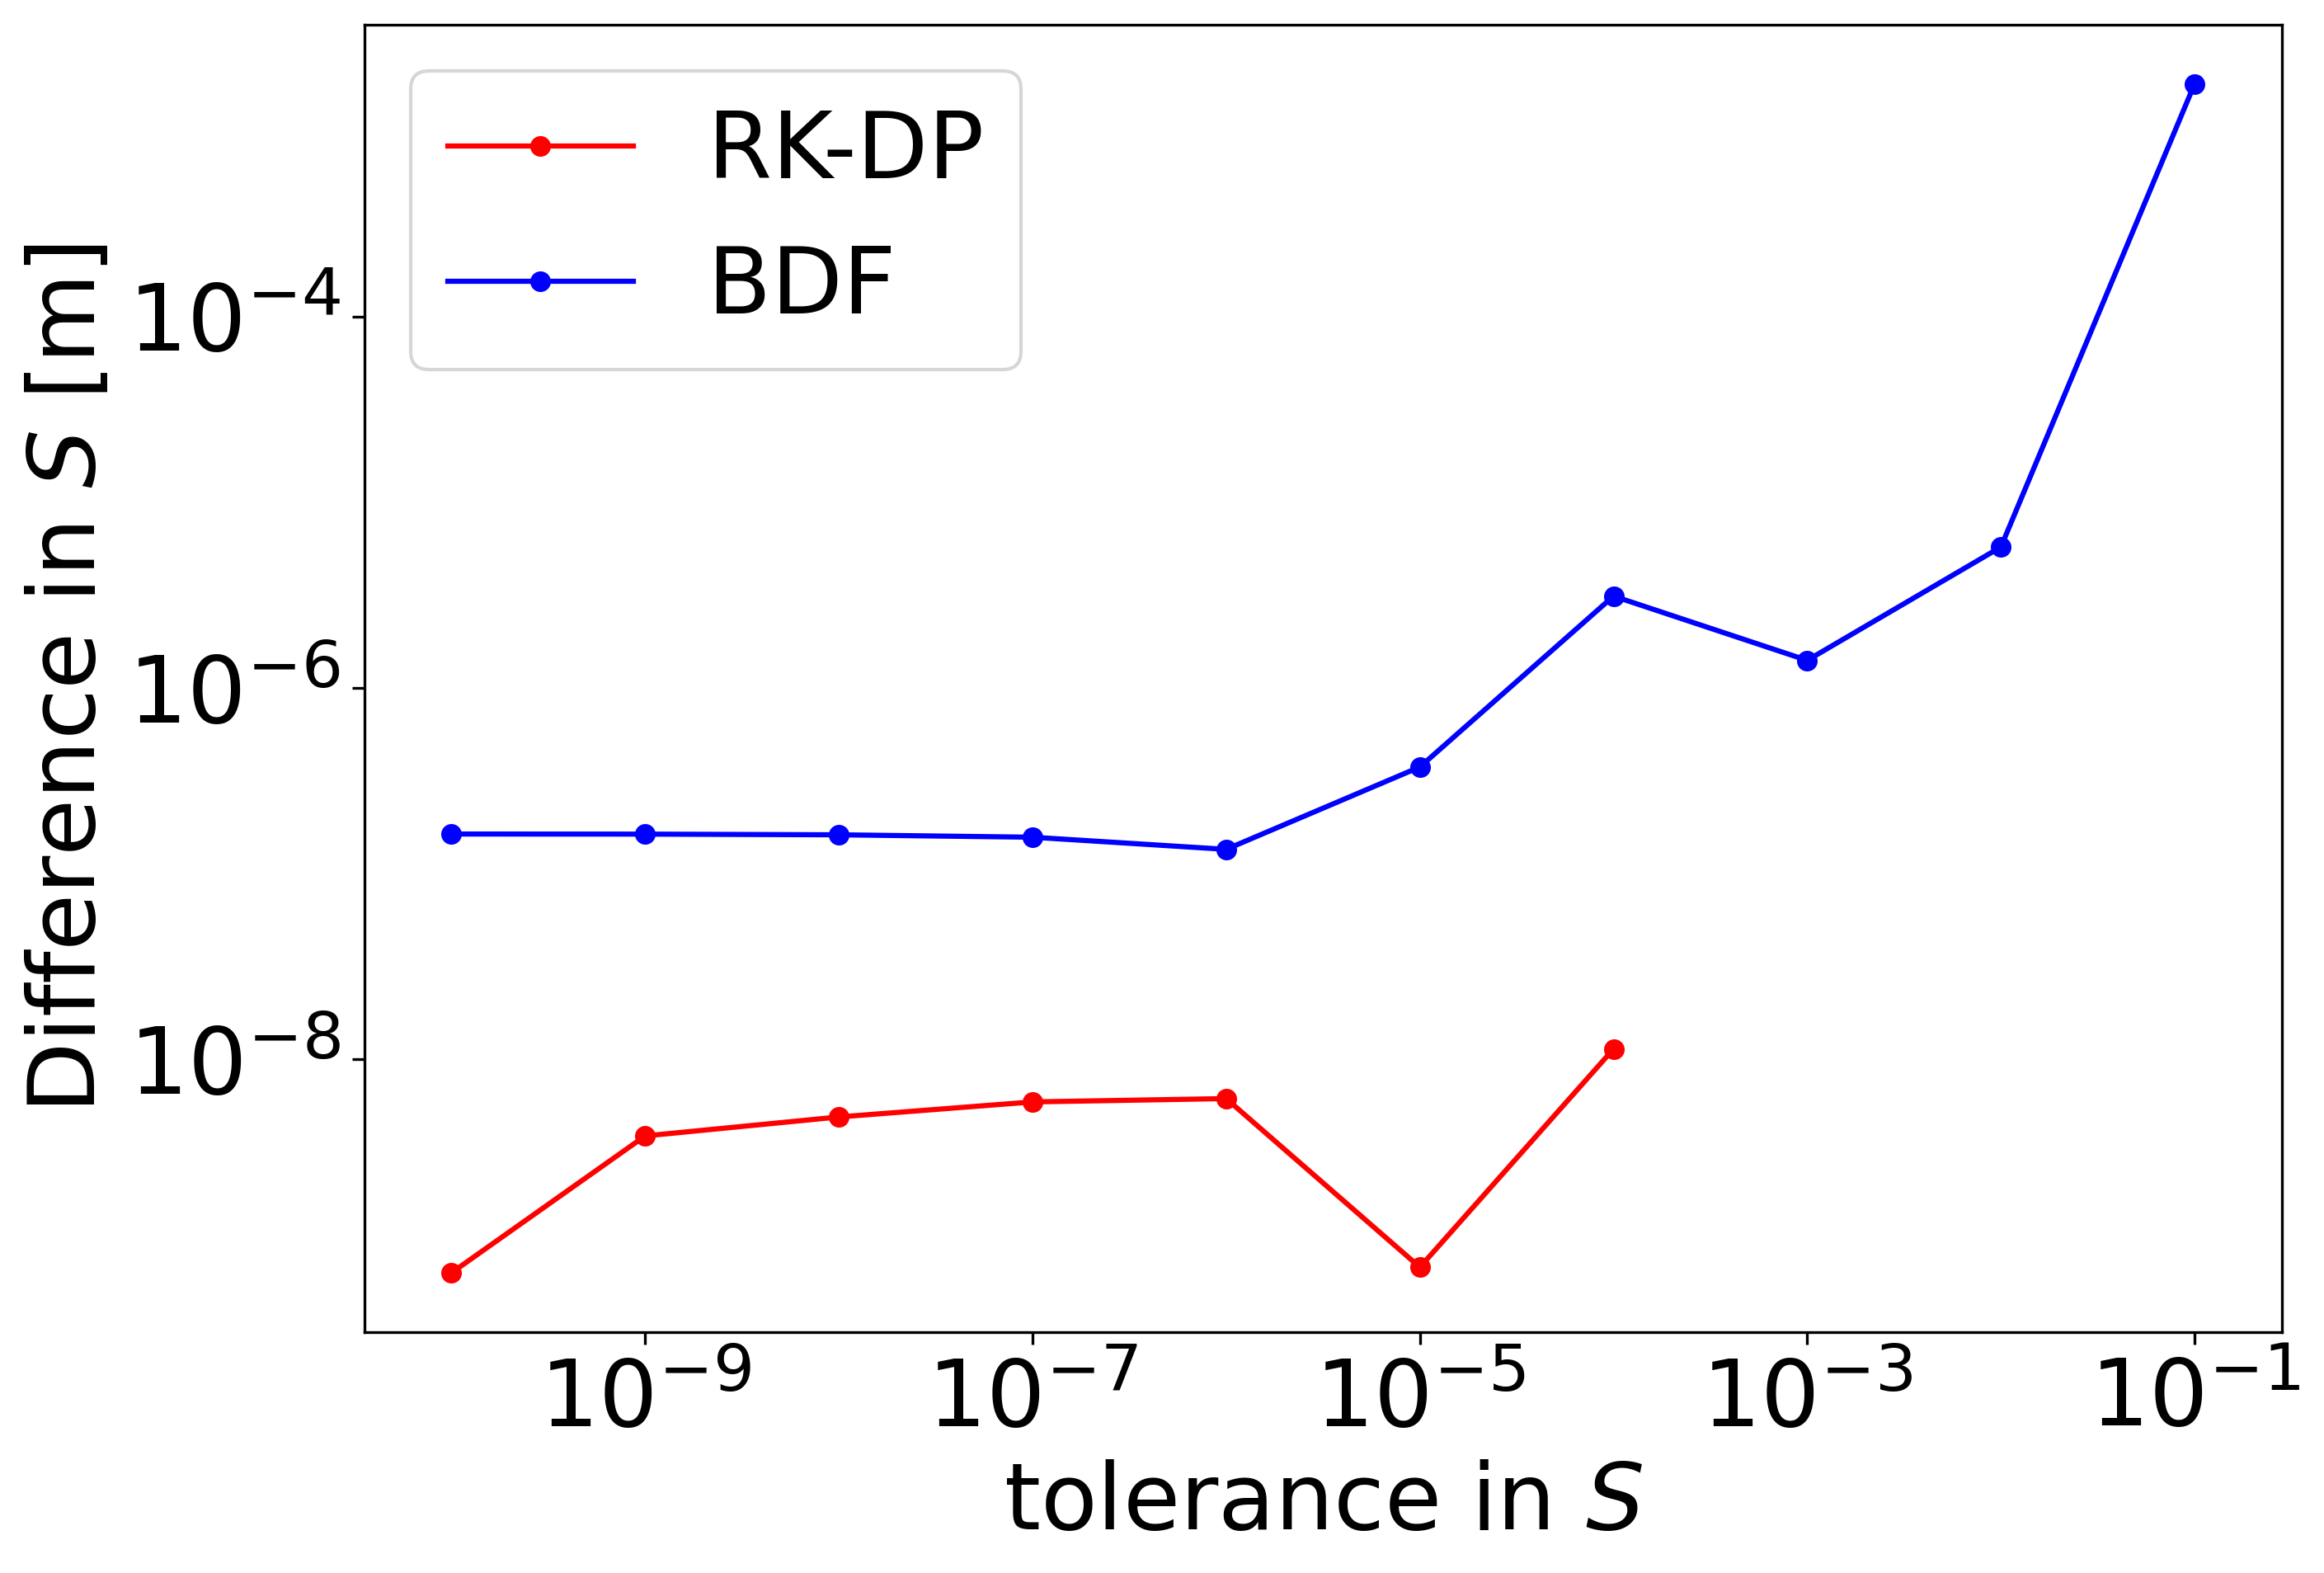
\includegraphics[width=1\textwidth]{images/TANDEMcompactODEDifferentTolerancesSize101_EQ_Smin.png}
		\subcaption{Difference in the slip increase} 
	\end{subfigure}
	\begin{subfigure}[t]{0.32\textwidth}
		\centering
		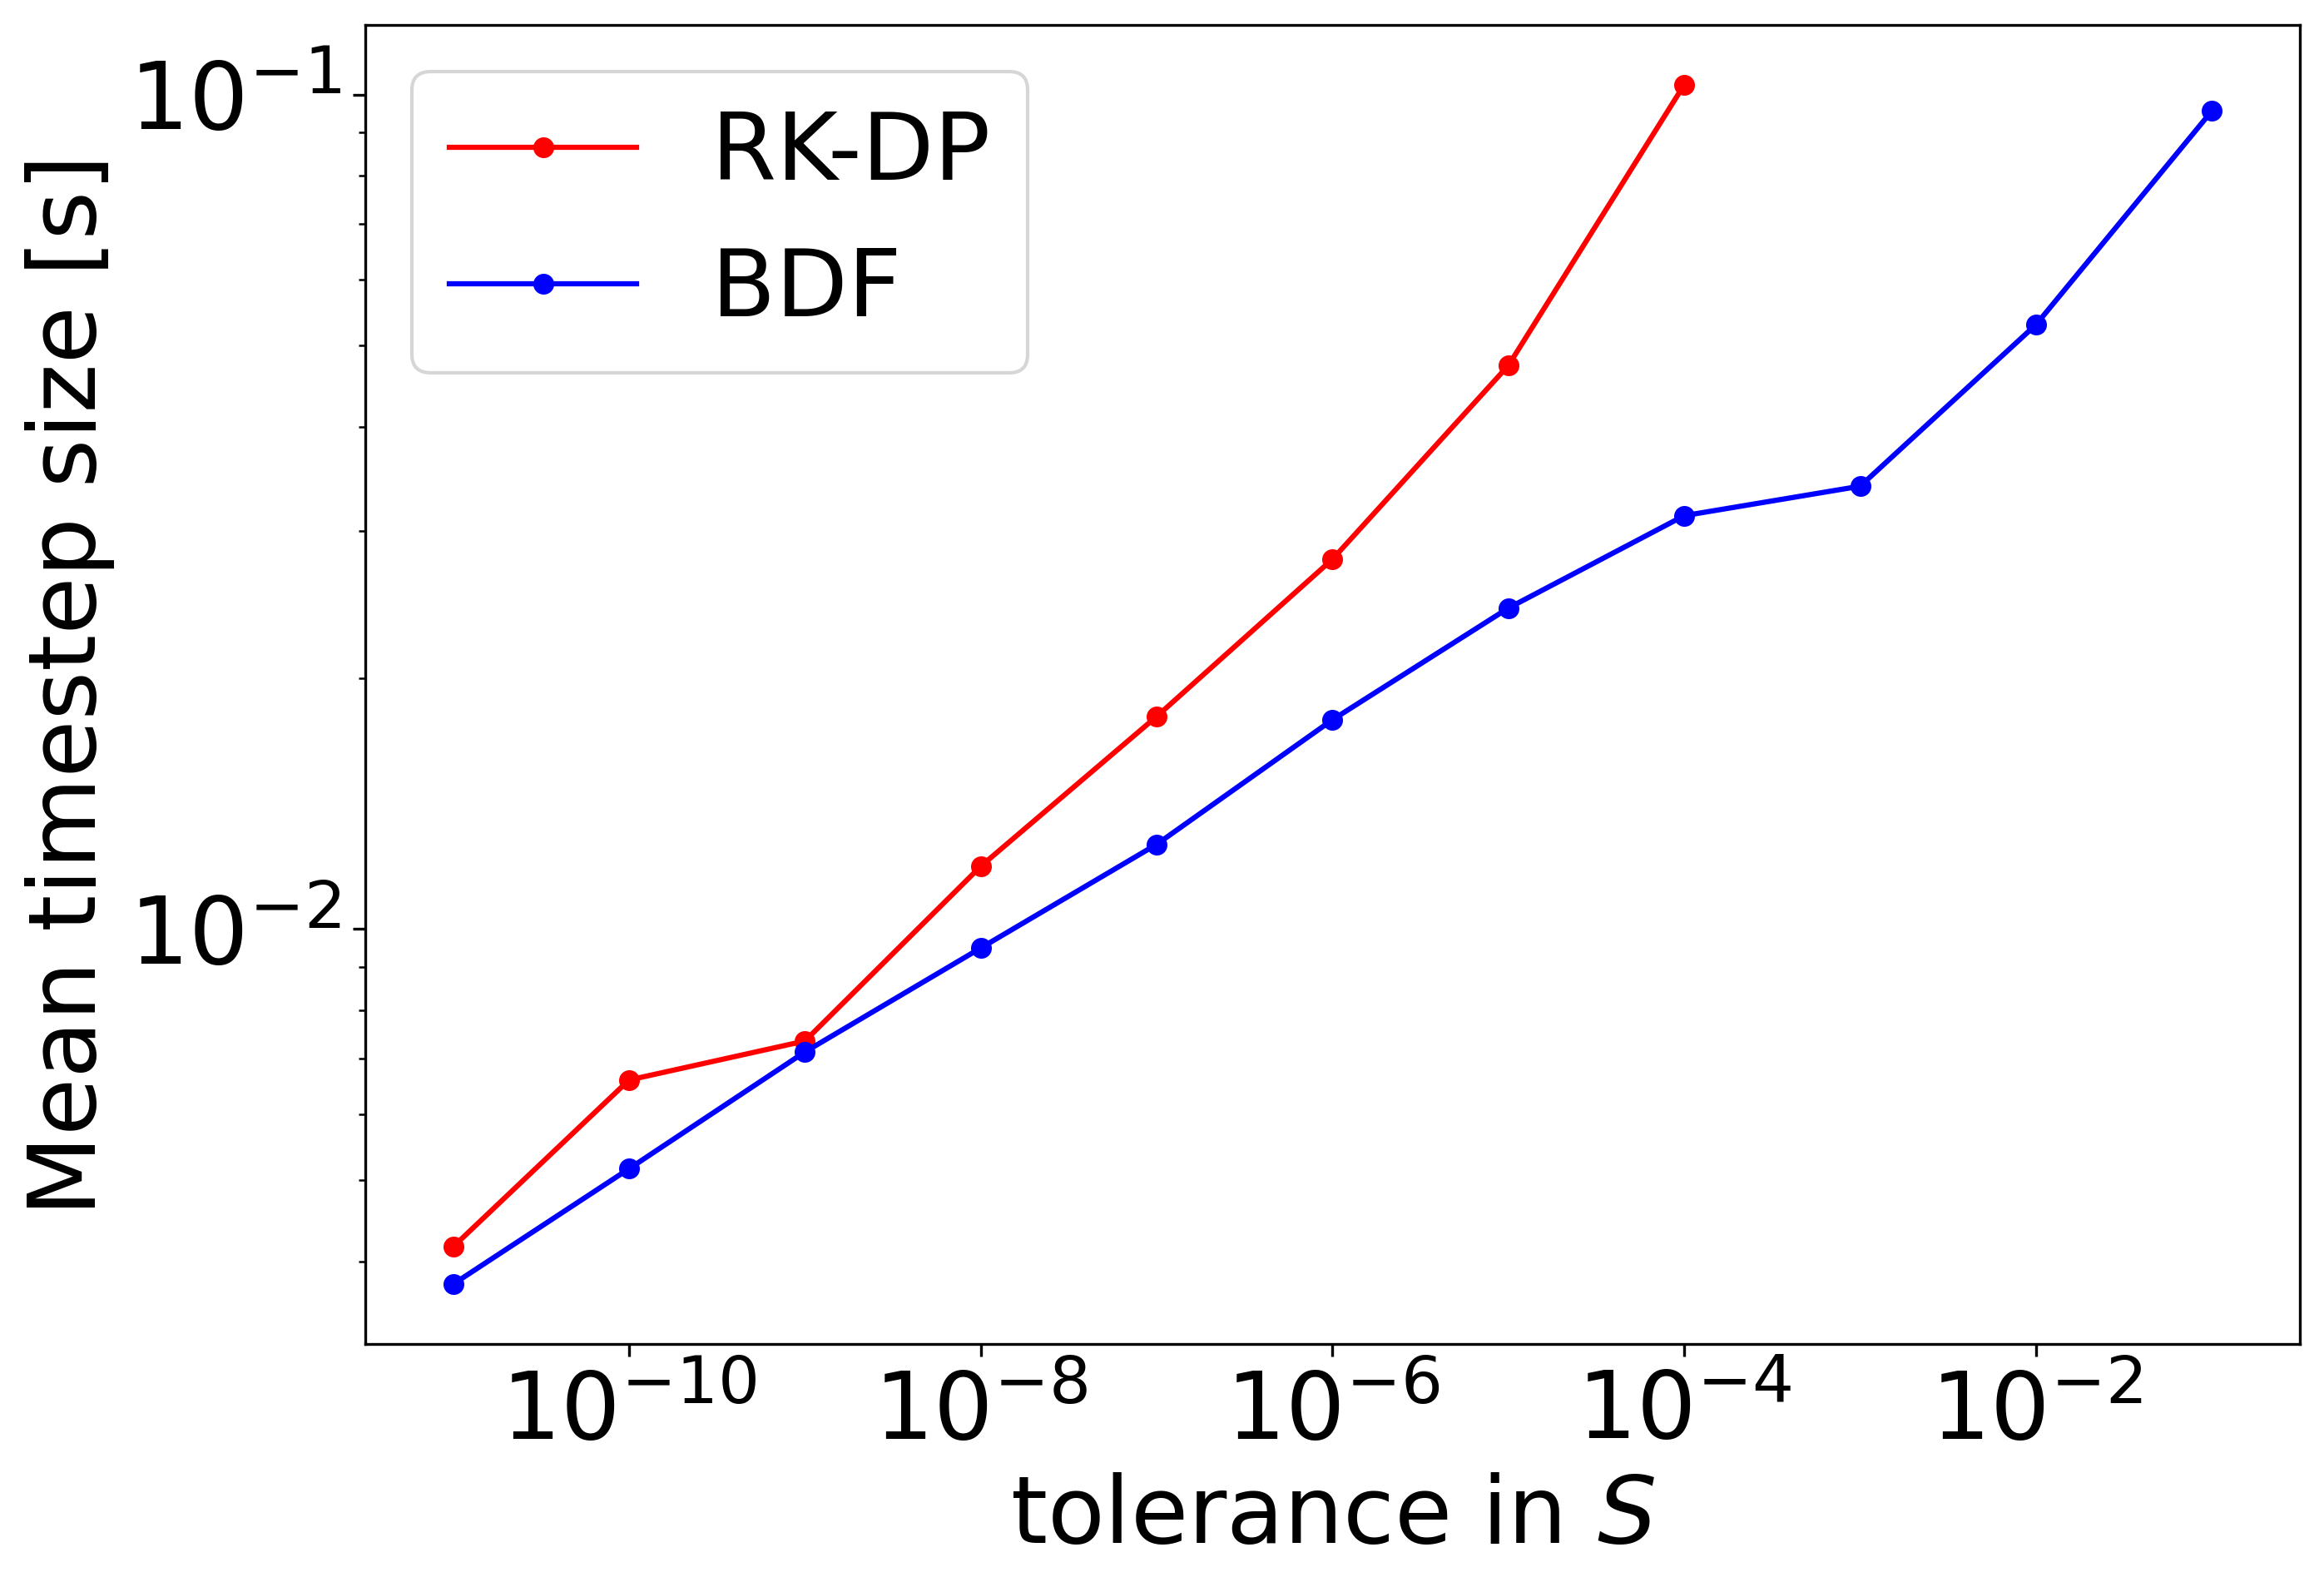
\includegraphics[width=1\textwidth]{images/TANDEMcompactODEDifferentTolerancesSize101_EQ_DT.png}
		\subcaption{Geometric mean of the timestep size in the earthquake} 
	\end{subfigure}
	\caption{Difference of characteristic quantities to the reference solution for different tolerances in the earthquake for a domain with 101 fault elements with the 1st order ODE formulation}
	\label{fig:tolerancesEarthquake_compactODE}
\end{figure}
The slip induced by the earthquake is predicted in general with a very high accuracy. Stricter tolerances cannot ameliorate the results as the error for the slip stagnates around $10^{-8}$ with the RK method and around $10^{-7}$ with the BDF method. The fact that the explicit method is more exact than the implicit one is due to the condition of the Newton iteration and has already been discussed in \autoref{ssec:StoppingCriterionNewton}. Only after the RK method fails to converge at $t_a^S = 10^{-3}$, the accuracy begins to deteriorate exponentially with BDF, but even for the last tested tolerance, the difference to the reference solution is of the order of millimeters. Considering that in the reference solution, most of the simulated time is spent in the earthquake, it is strongly recommended to choose a much lower tolerance than for the aseismic slip. One big advantage of implicit methods here is that they return conclusive results even when explicit methods already failed. \\

In both earthquakes and aseismic phases, the timestep size increases logarithmically with the tolerance. With RK-DP, to increase the timestep size by one order of magnitude, the tolerance has to be four orders larger, which reflects the 4th order accuracy of the scheme. Simarly, for the BDF method, the ratio is six to one, which indicates that the order adapter chooses the BDF6 for most of the steps. However, prescribing a lower BDF order would not scale the timesteps faster up, as the adaptive-order finding already optimizes the time-step size. \\

The extended DAE formulation behaves essentially the same as the BDF method in the graphs above, and the compact DAE only for the aseismic slip, since it diverges in earthquakes. The 2nd order ODE formulation differs by the fact that it is driven by the state variable $\psi$ and the slip rate $V$, and the same set of experiments has been repeated, but for varying relative tolerances in $V$. The reference solution is set to $t_r^V=10^{-11}$, the error in the aseismic phase is shown in \autoref{fig:tolerancesAseismicSlip_extendedODE} and in the earthquake in \autoref{fig:tolerancesEarthquake_extendedODE}.
\begin{figure}[H]
	\centering
	\begin{subfigure}[t]{0.32\textwidth}
		\centering
		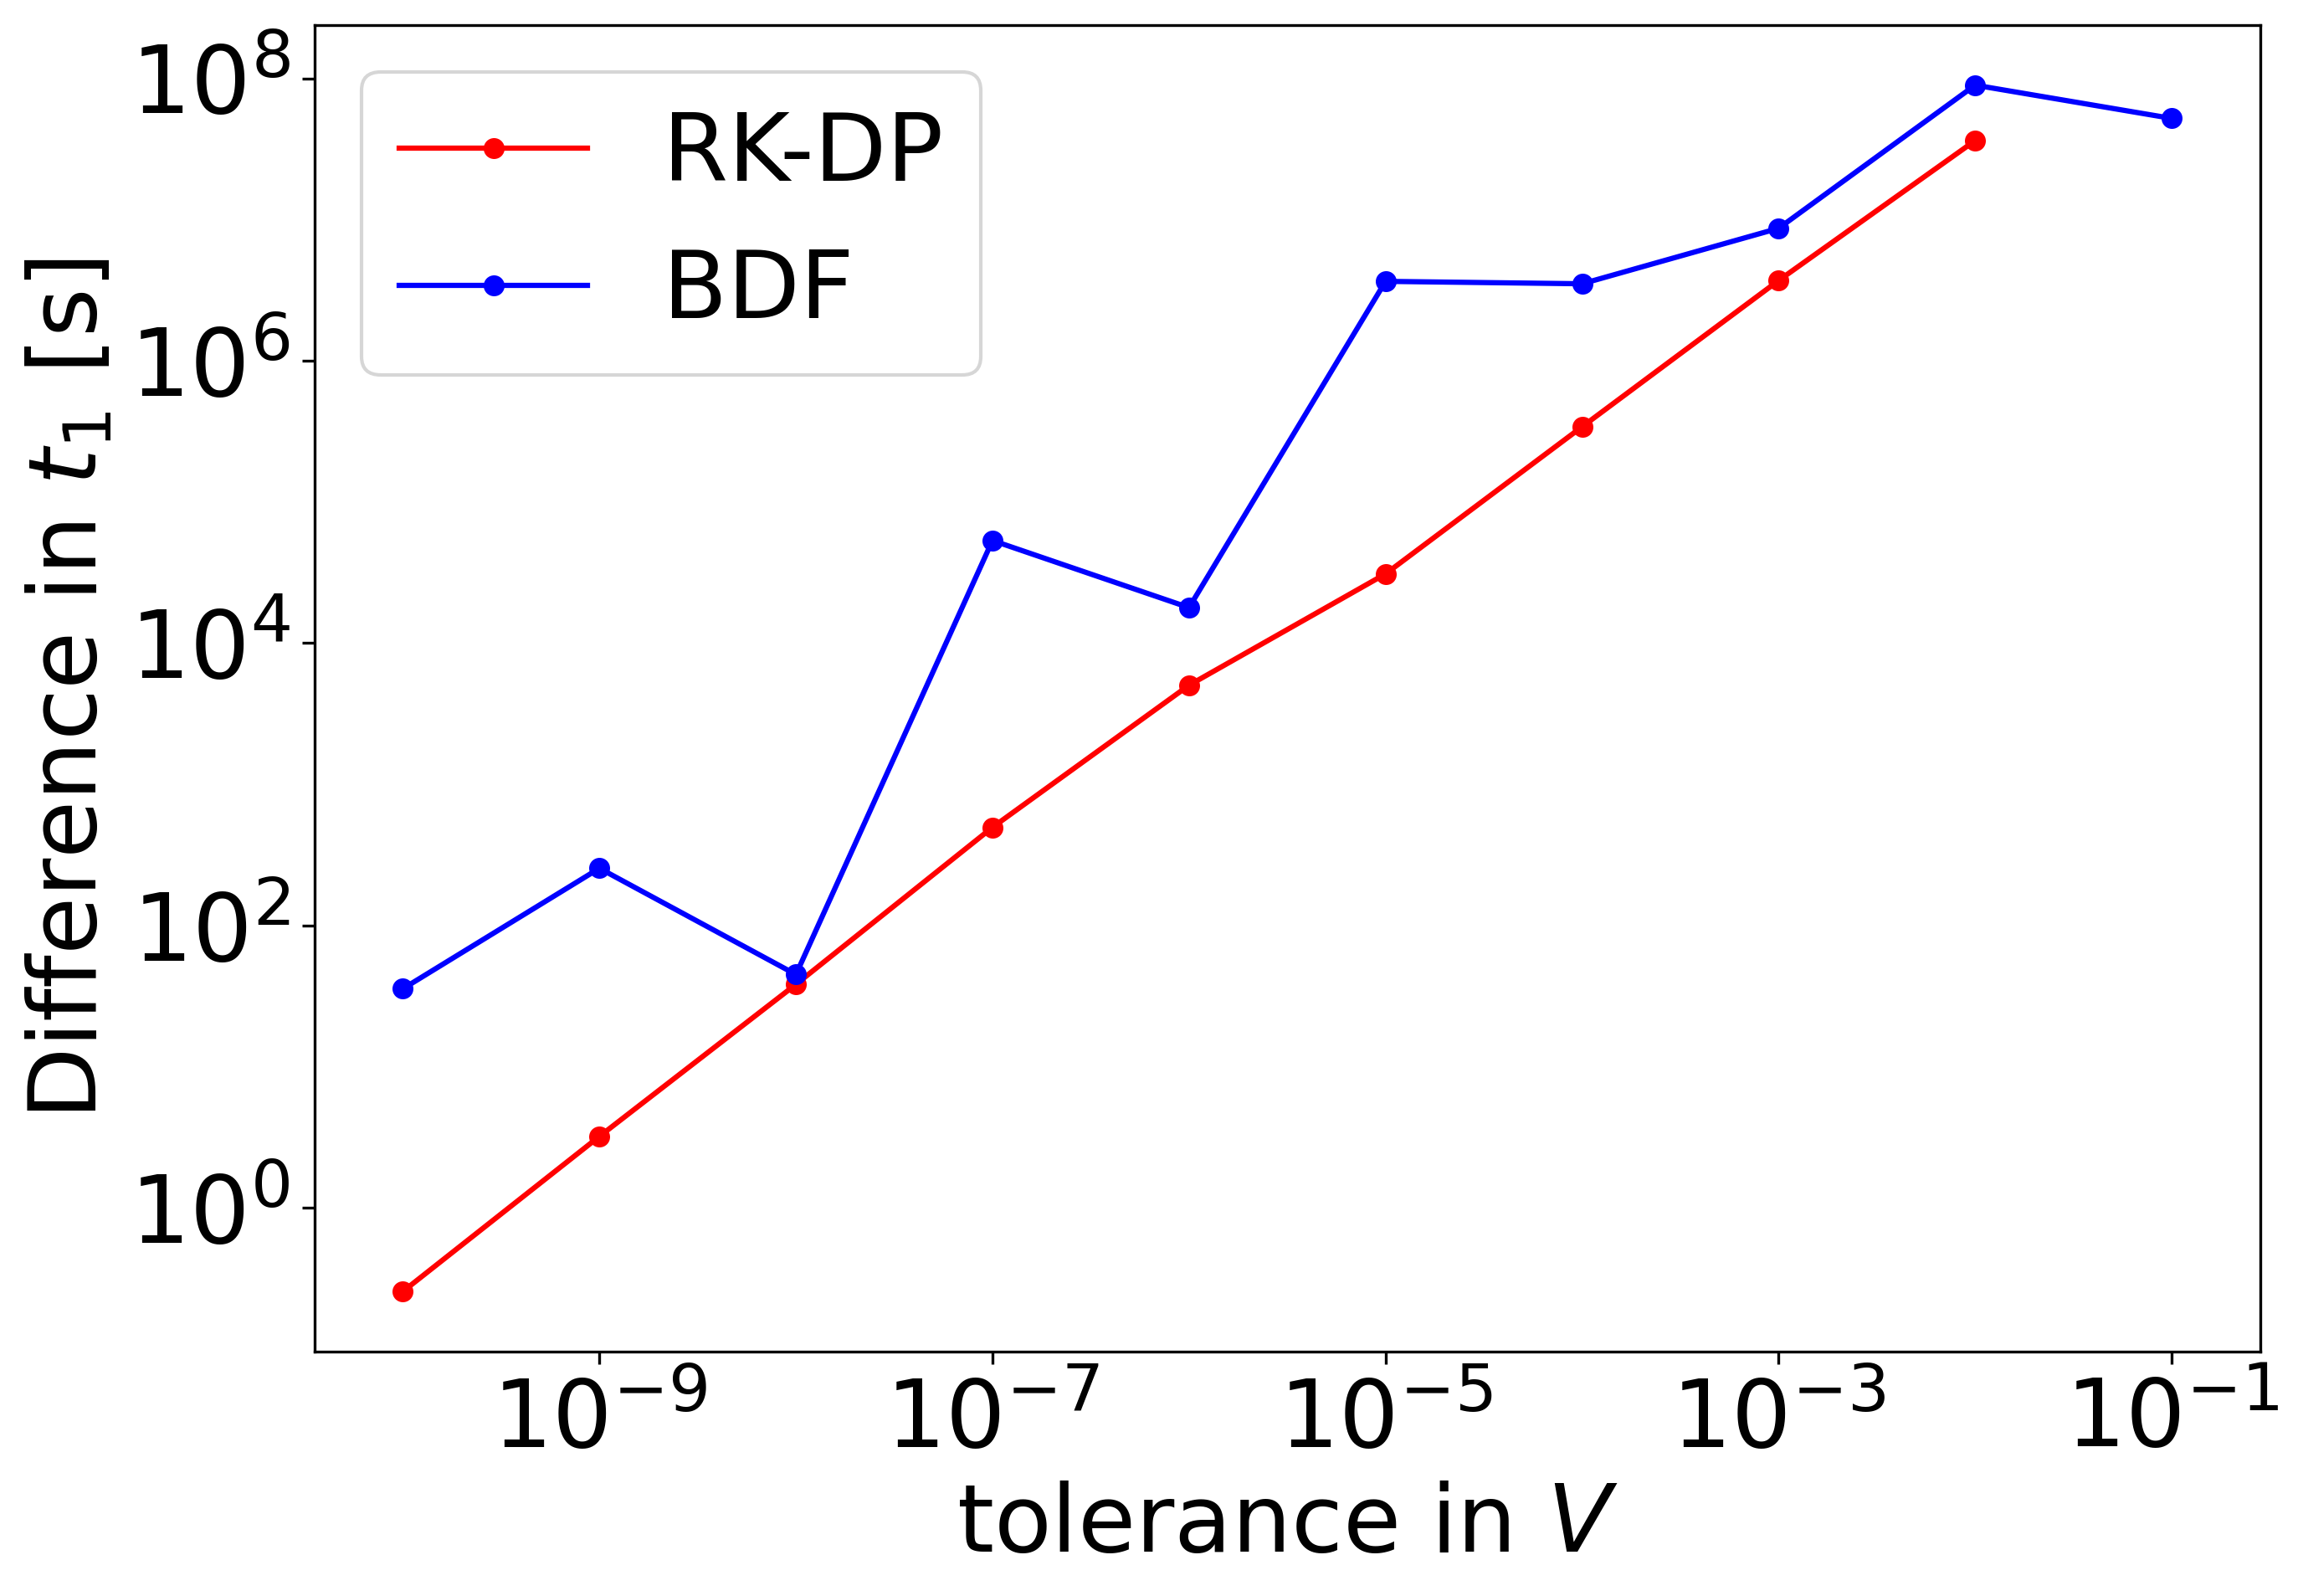
\includegraphics[width=1\textwidth]{images/TANDEMextendedODEDifferentTolerancesSize101_AS_FirstEarthquakeTimeDiff.png}
		\subcaption{Time difference of the first earthquake} 
	\end{subfigure} 
	\begin{subfigure}[t]{0.32\textwidth}
		\centering
		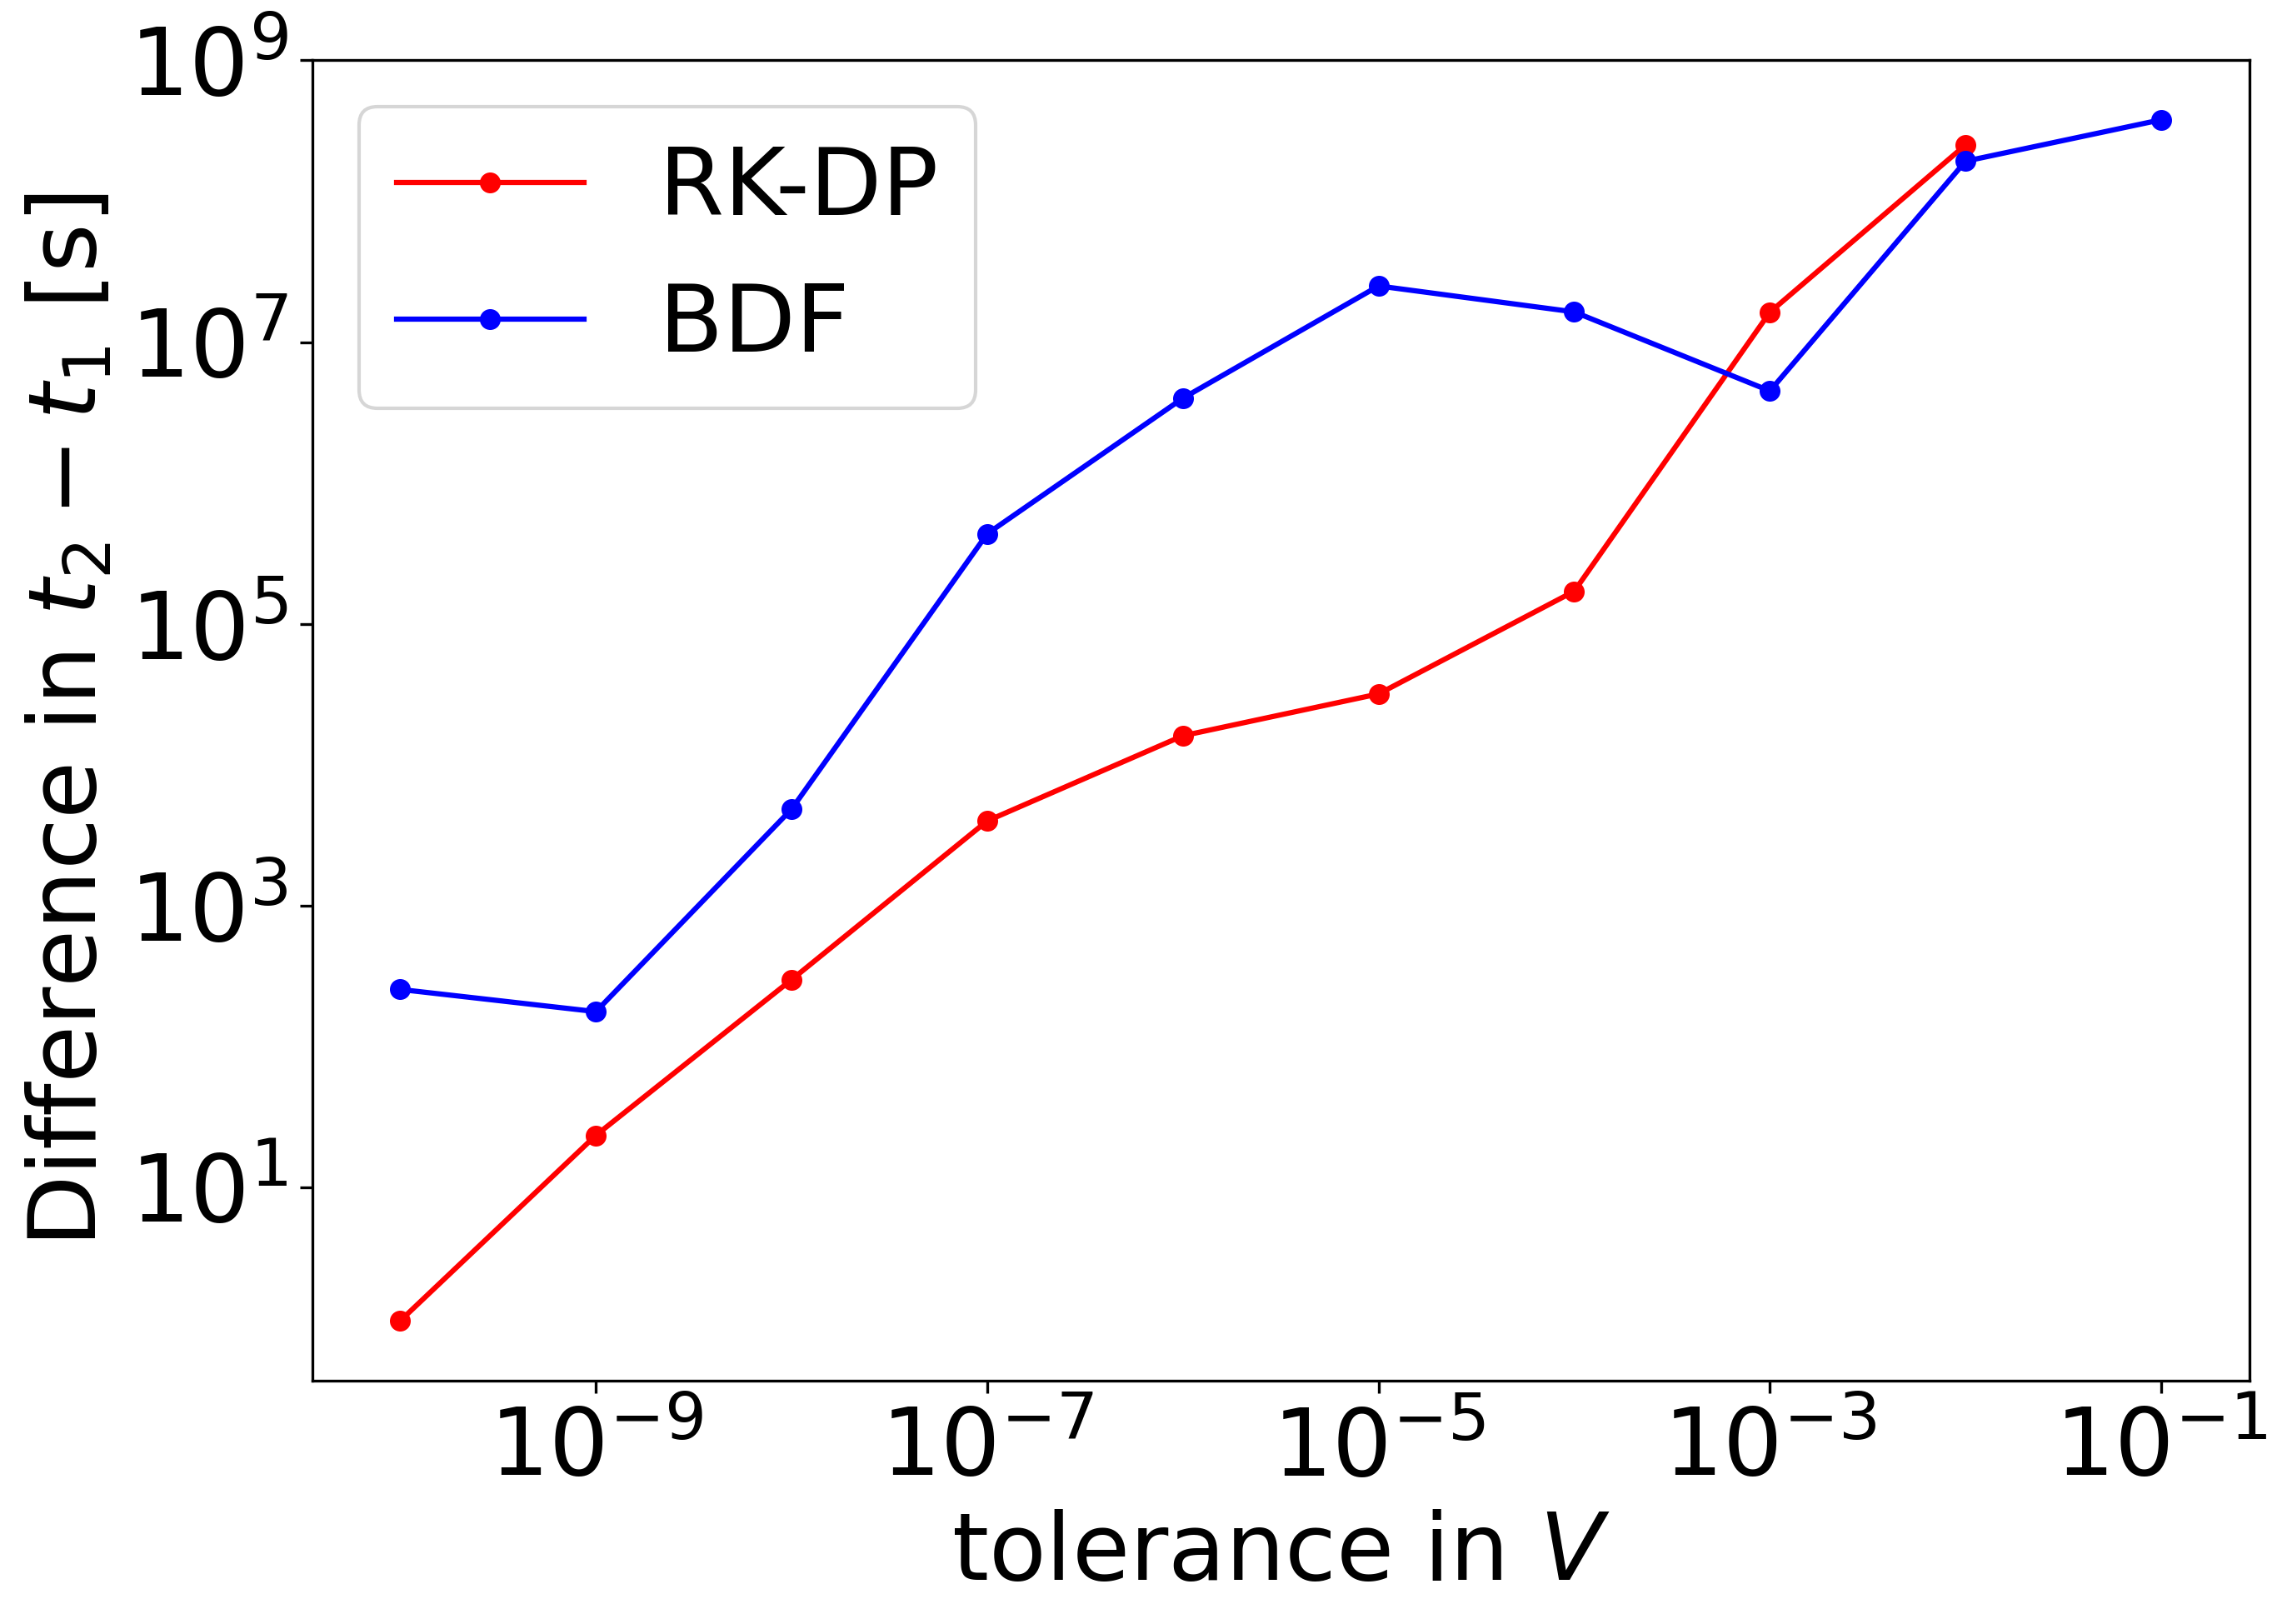
\includegraphics[width=1\textwidth]{images/TANDEMextendedODEDifferentTolerancesSize101_AS_PeriodDiff.png}
		\subcaption{Difference of the period between both earthquakes} 
	\end{subfigure}
	\begin{subfigure}[t]{0.32\textwidth}
		\centering
		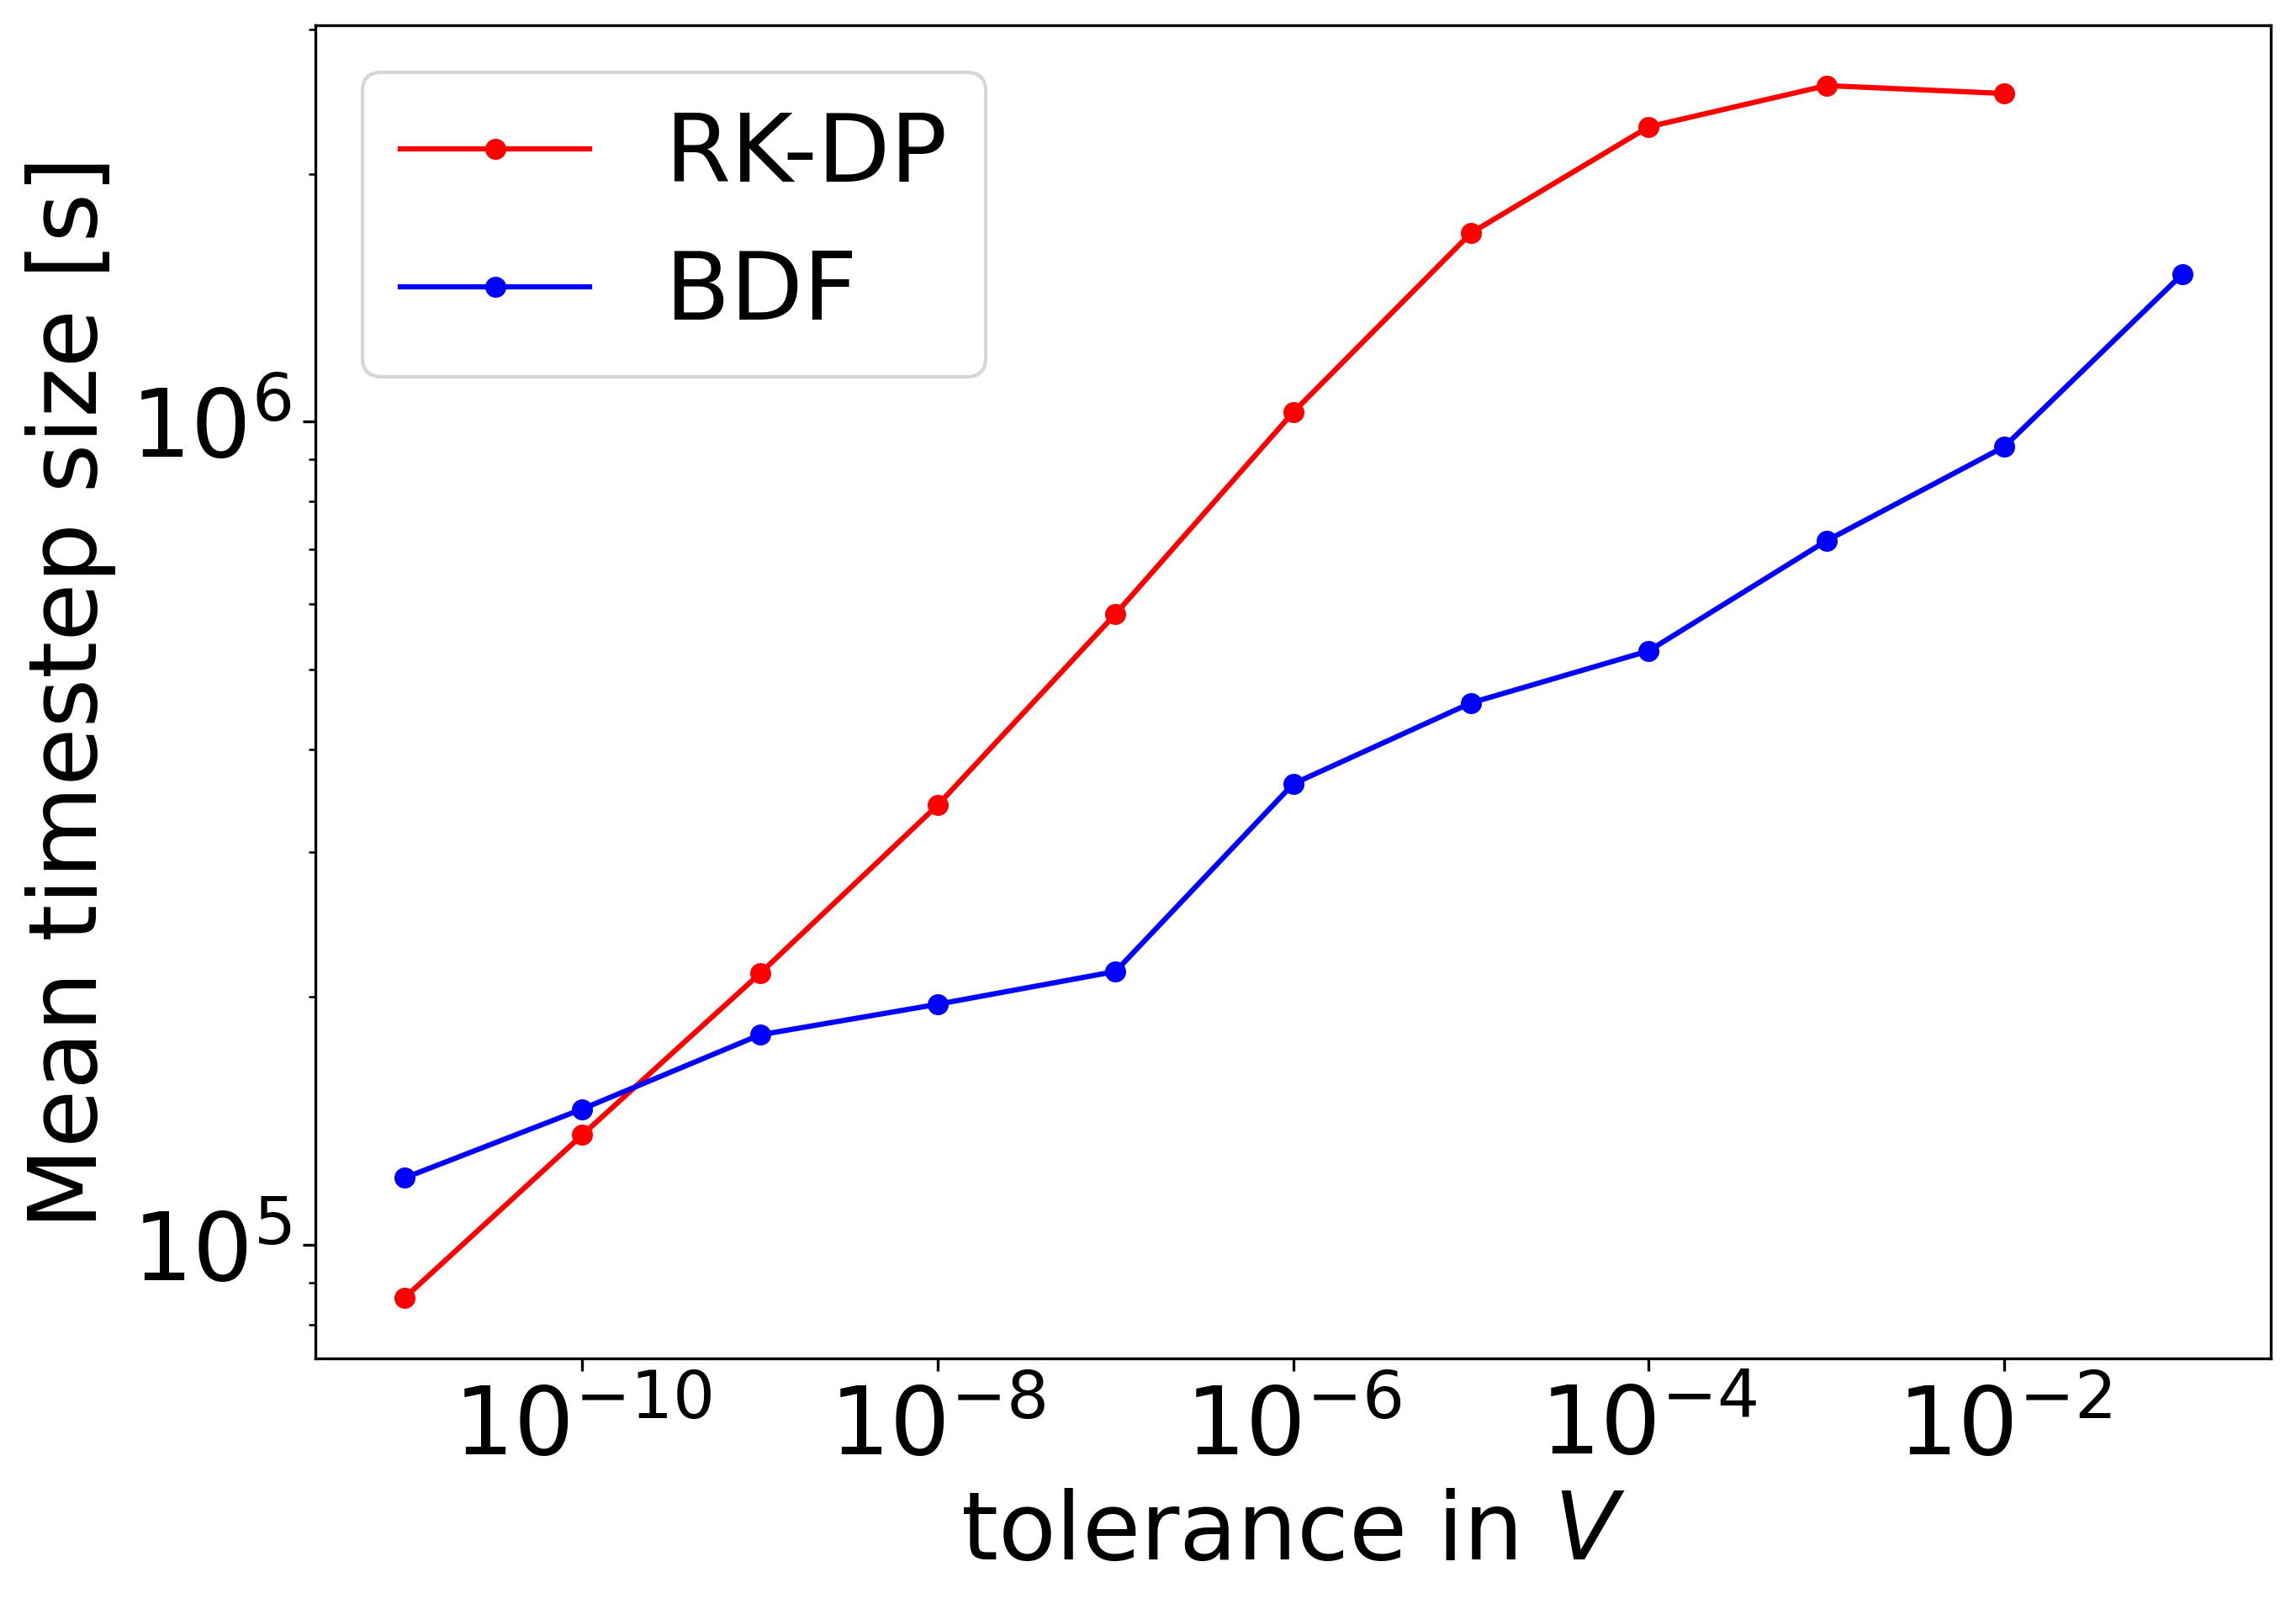
\includegraphics[width=1\textwidth]{images/TANDEMextendedODEDifferentTolerancesSize101_AS_DT.png}
		\subcaption{Geometric mean of the timestep size in the aseismic slip} 
	\end{subfigure}
	\caption{Difference of characteristic times to the reference solution for different tolerances in the aseismic slip phase for a domain with 101 fault elements with the 2nd order ODE formulation}
	\label{fig:tolerancesAseismicSlip_extendedODE}
\end{figure}



\begin{figure}[H]
	\centering
	\begin{subfigure}[t]{0.32\textwidth}
		\centering
		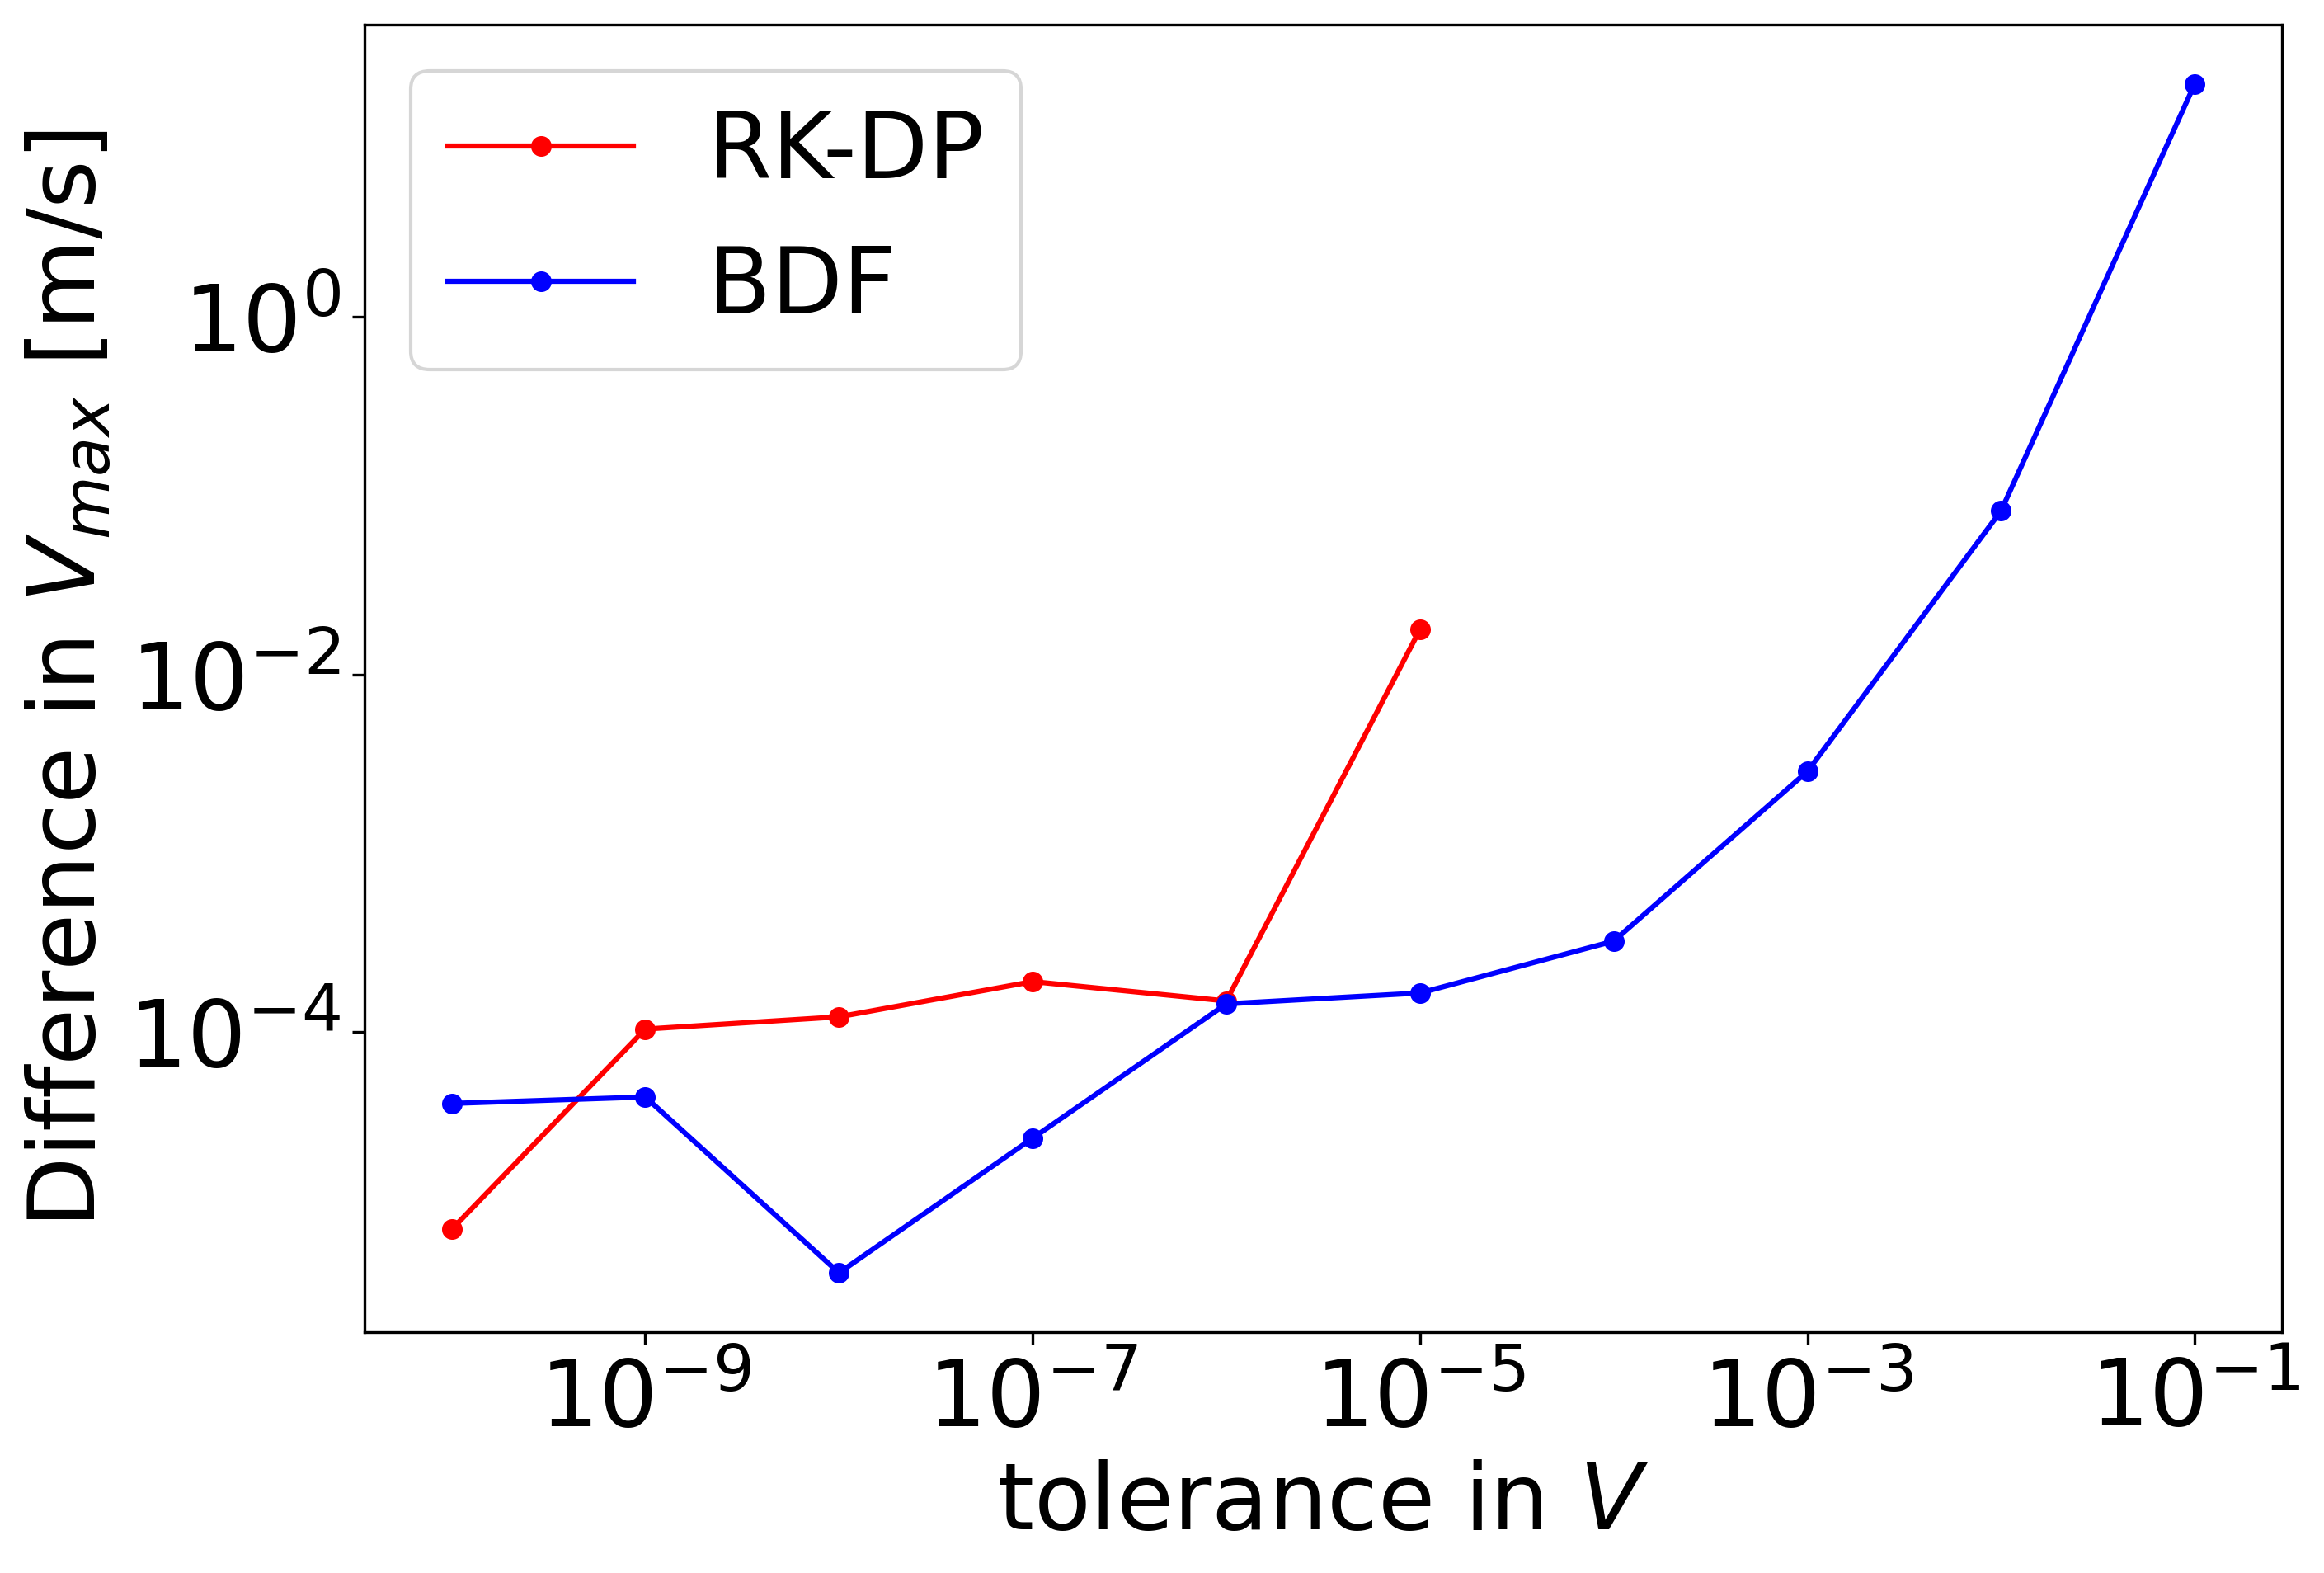
\includegraphics[width=1\textwidth]{images/TANDEMextendedODEDifferentTolerancesSize101_EQ_Vmax.png}
		\subcaption{Difference in the maximum slip rate} 
	\end{subfigure} 
	\begin{subfigure}[t]{0.32\textwidth}
		\centering
		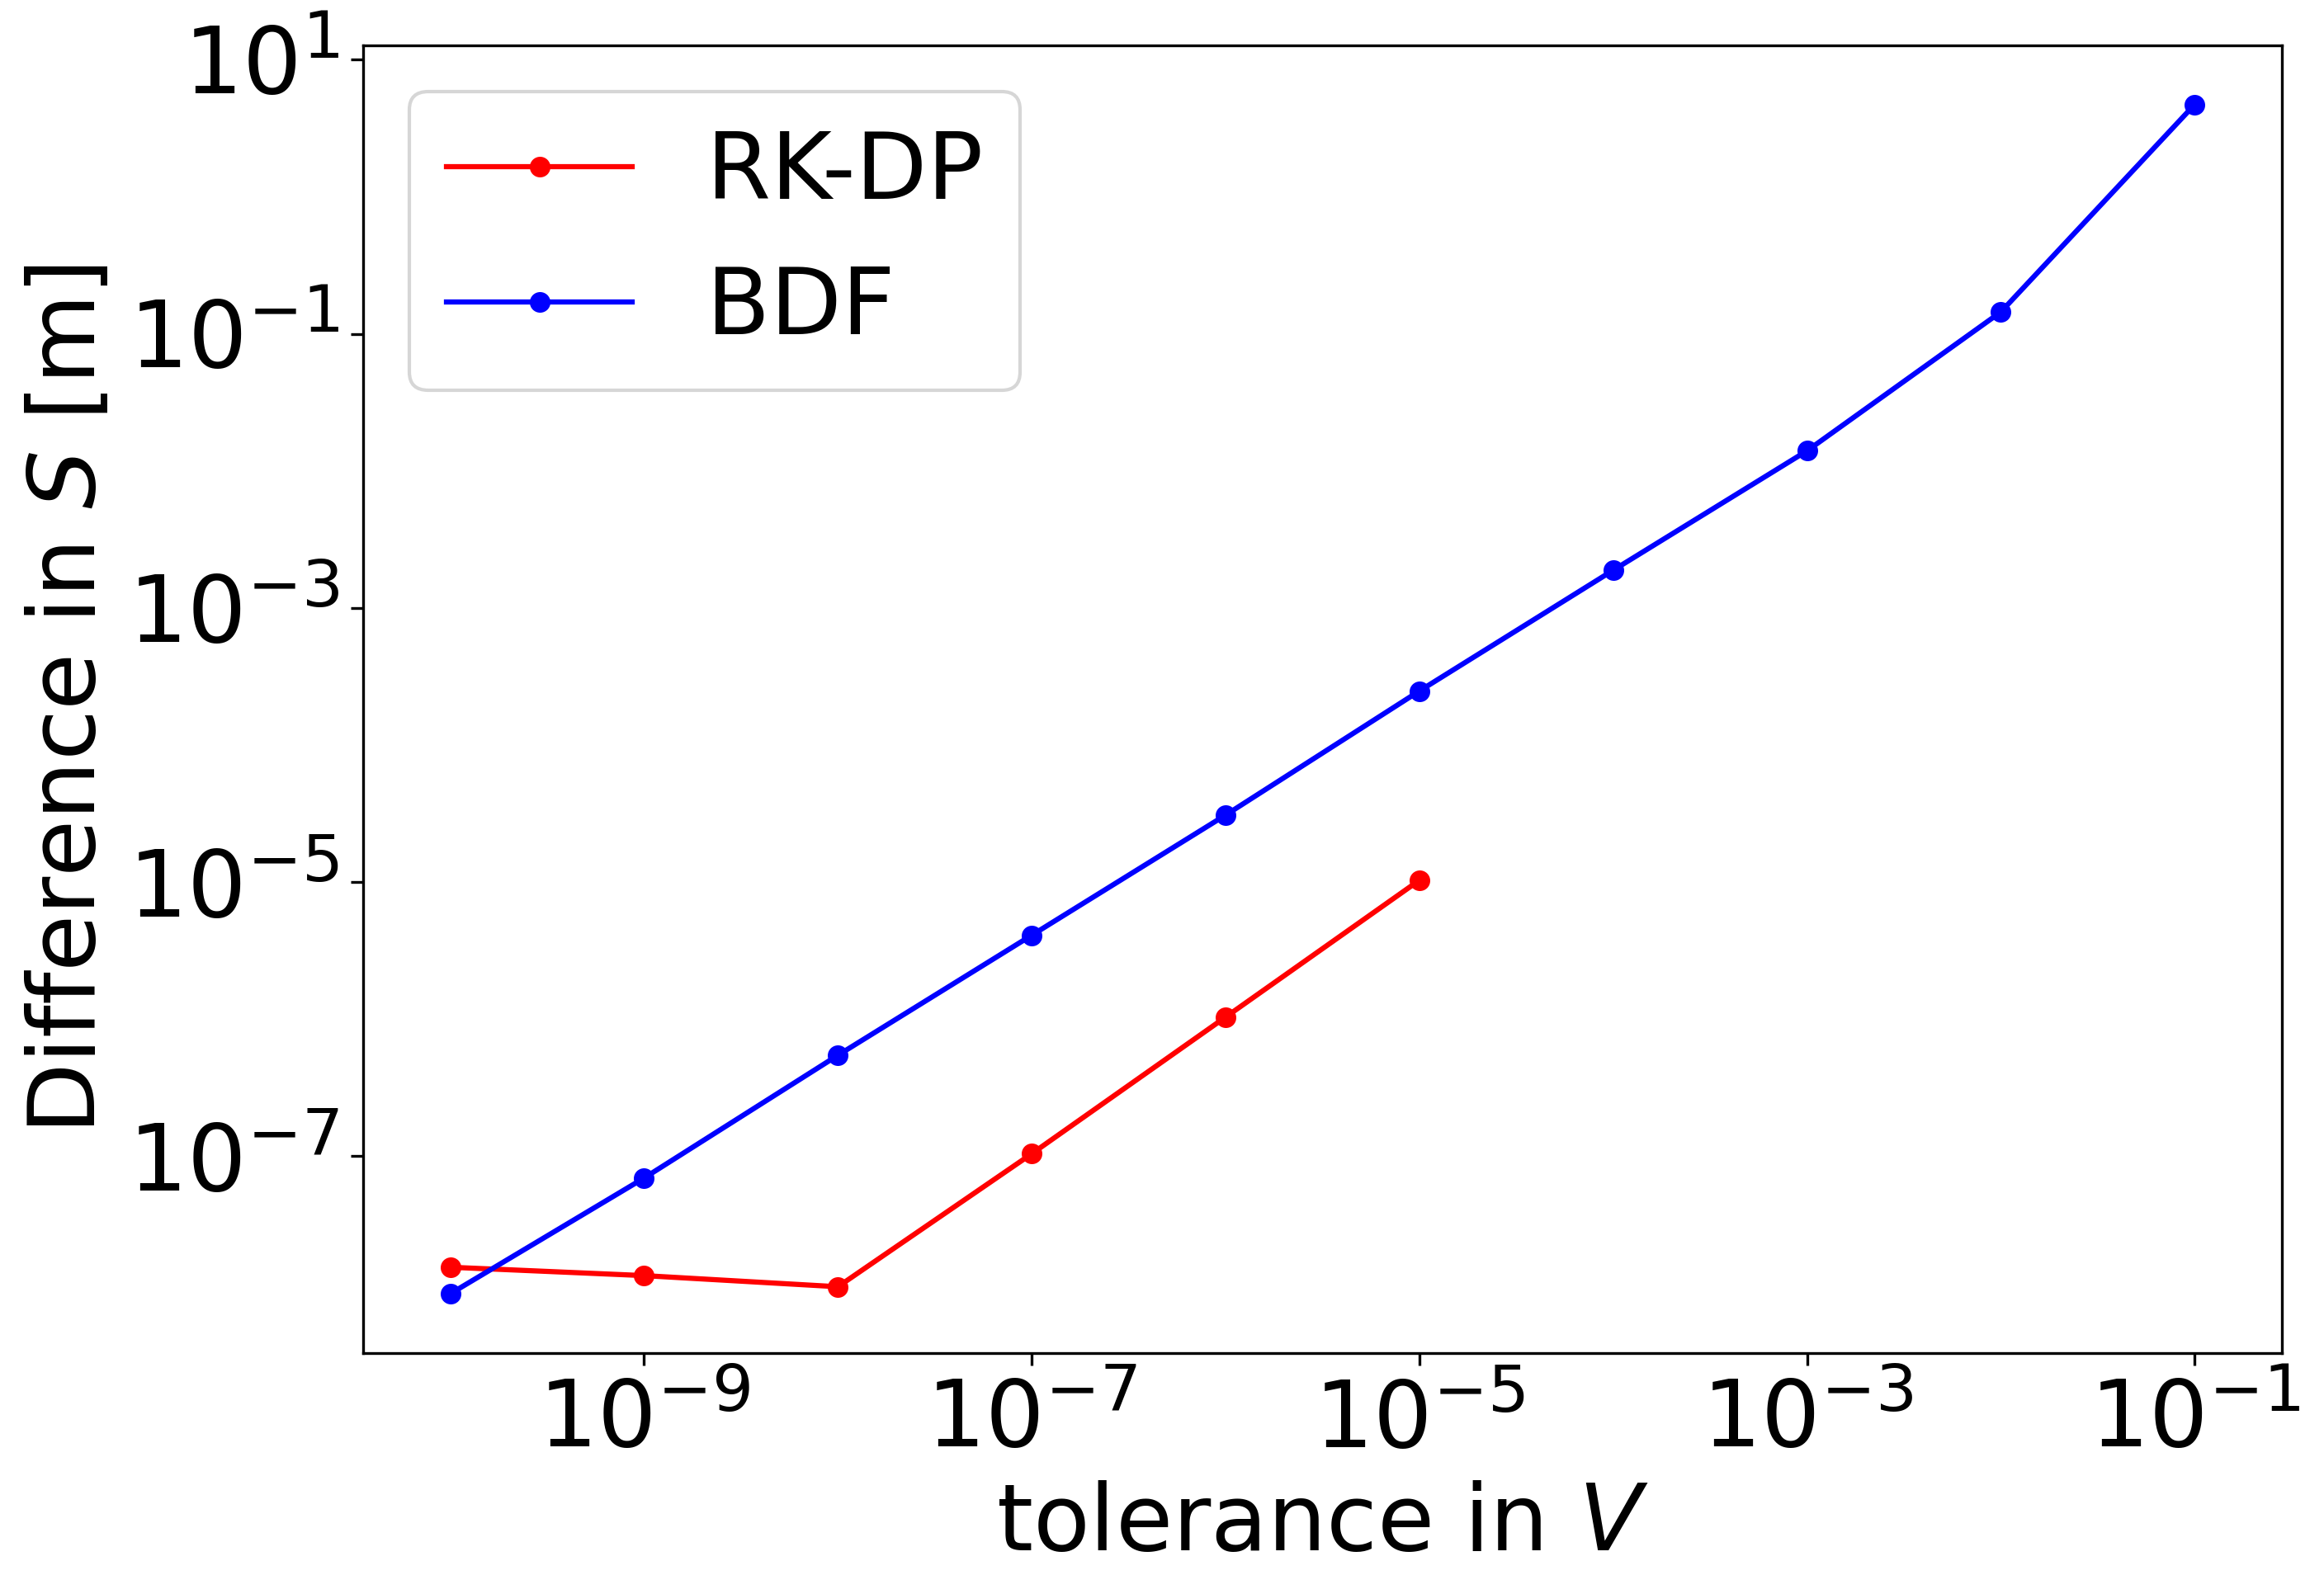
\includegraphics[width=1\textwidth]{images/TANDEMextendedODEDifferentTolerancesSize101_EQ_Smin.png}
		\subcaption{Difference in the slip increase} 
	\end{subfigure}
	\begin{subfigure}[t]{0.32\textwidth}
		\centering
		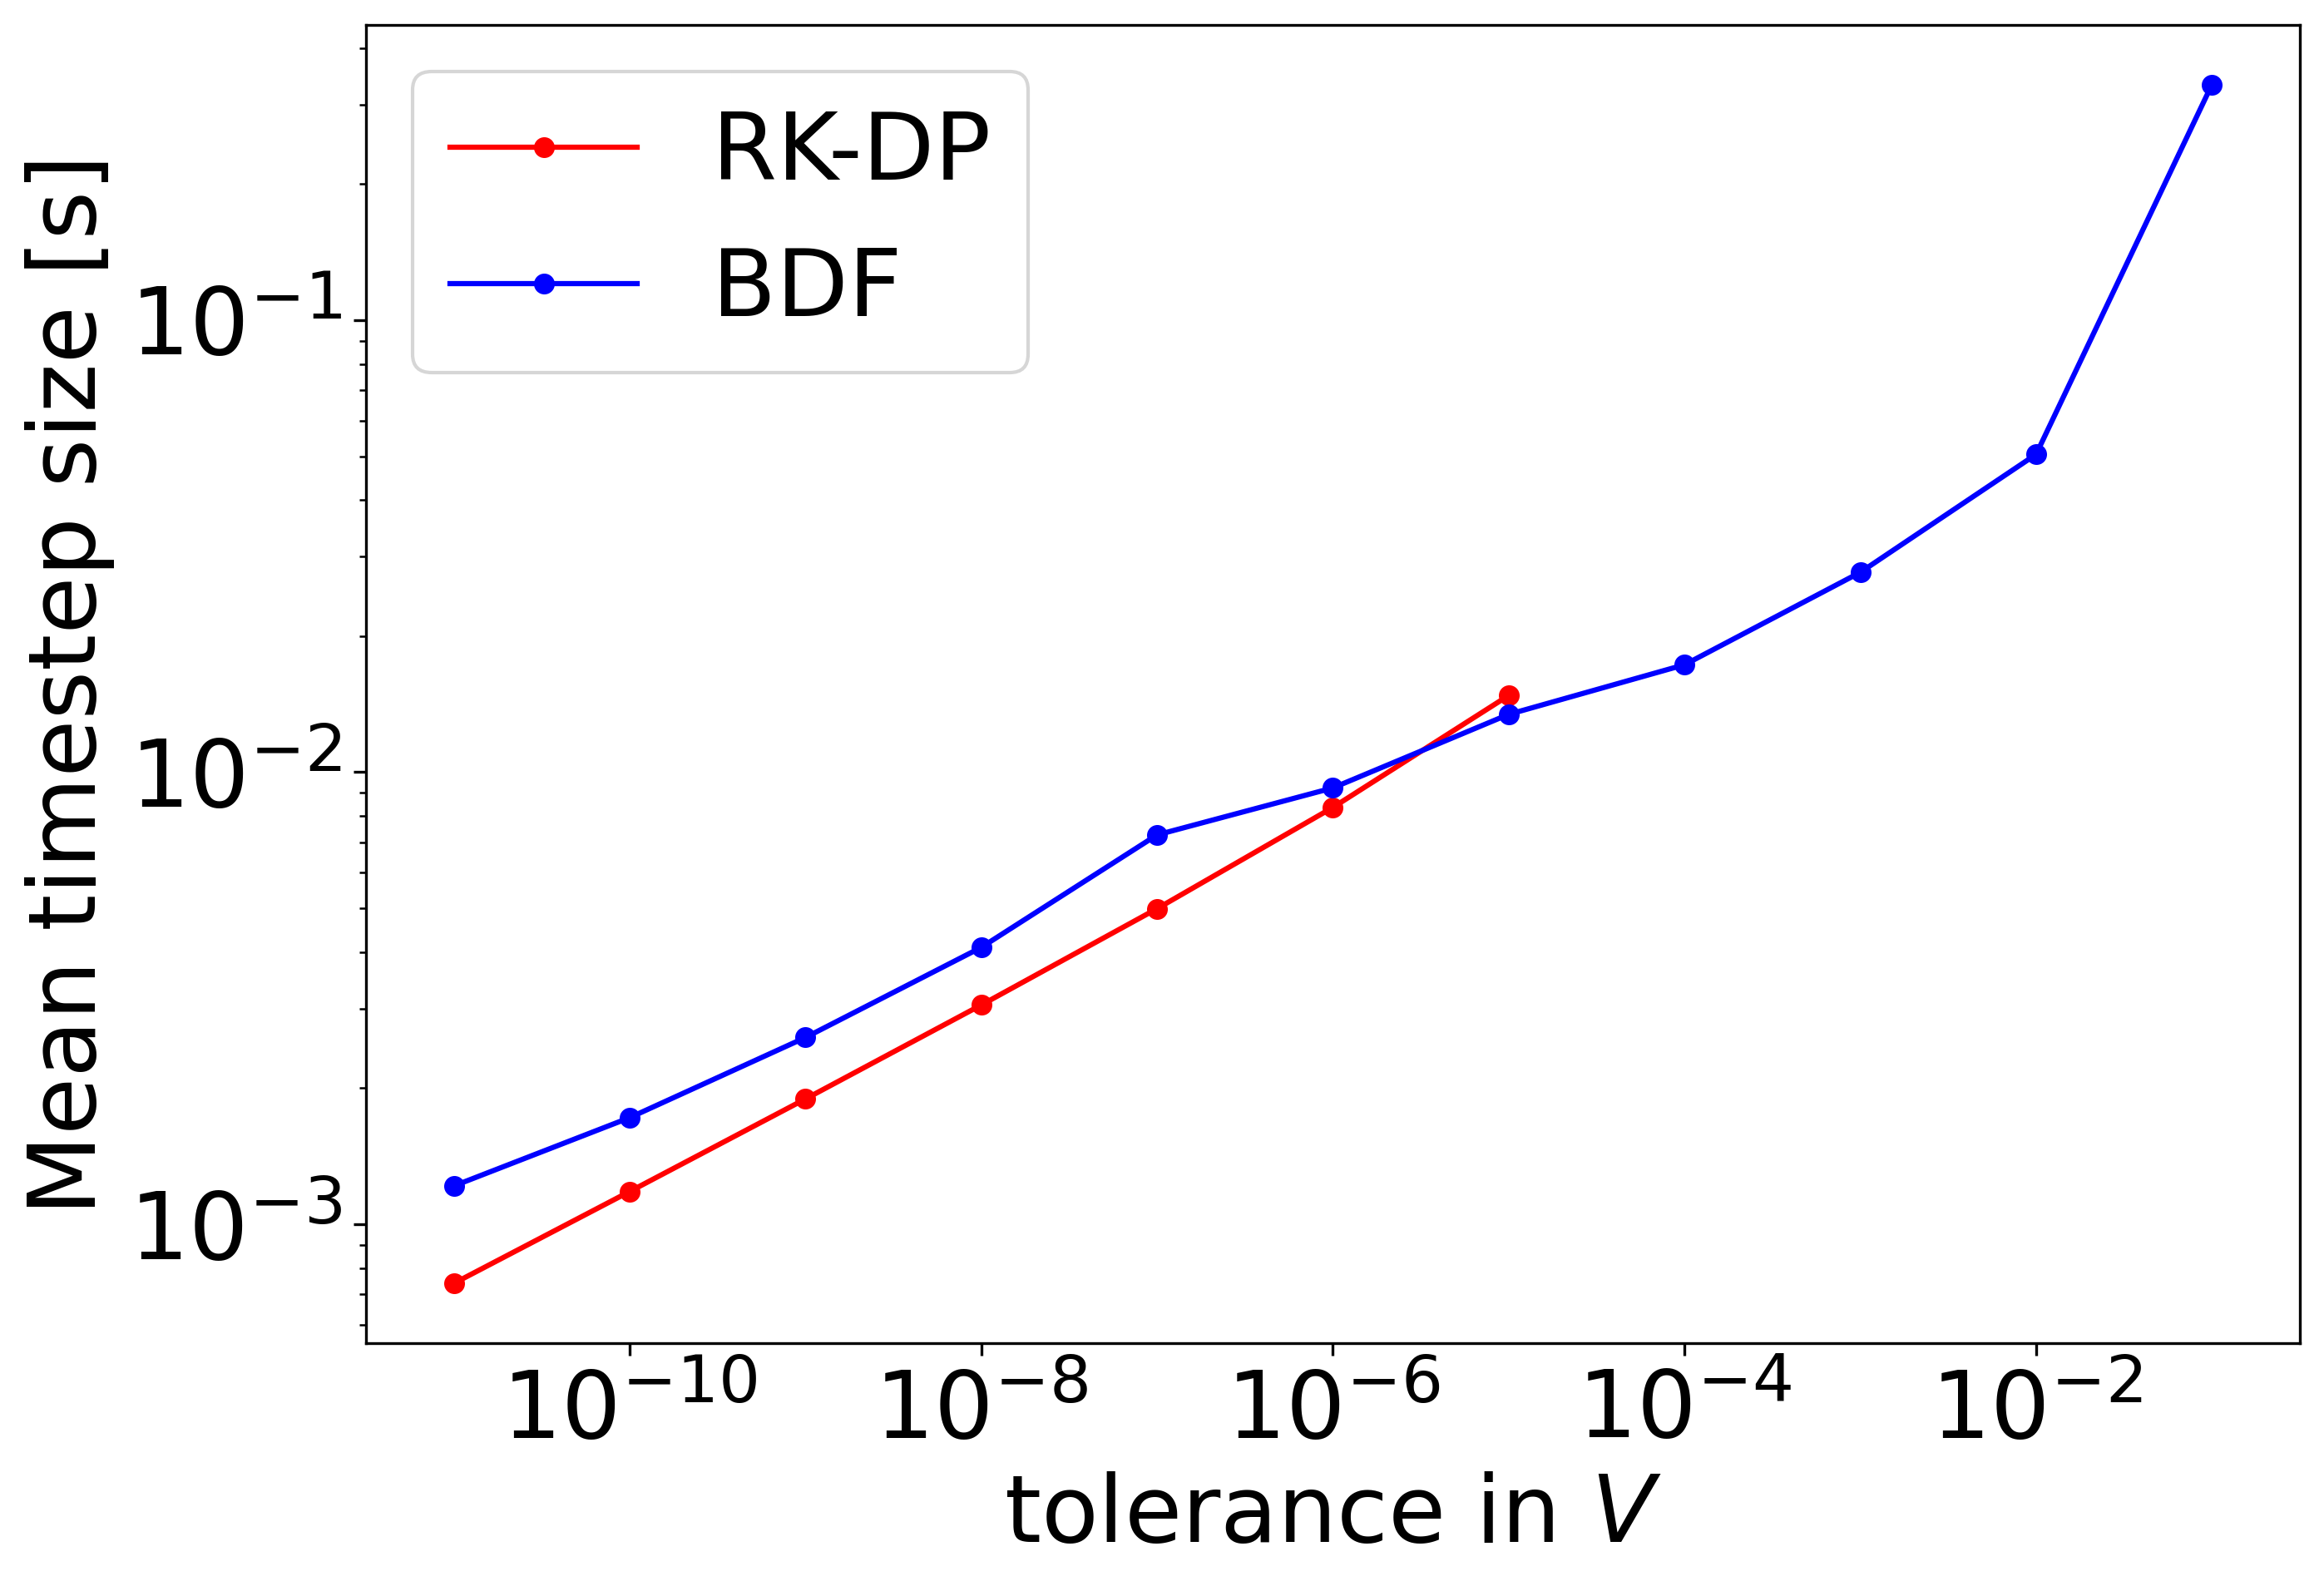
\includegraphics[width=1\textwidth]{images/TANDEMextendedODEDifferentTolerancesSize101_EQ_DT.png}
		\subcaption{Geometric mean of the timestep size in the earthquake} 
	\end{subfigure}
	\caption{Difference of characteristic quantities to the reference solution for different tolerances in the earthquake for a domain with 101 fault elements with the 2nd order ODE formulation}
	\label{fig:tolerancesEarthquake_extendedODE}
\end{figure}
Again, the accuracy increases with smaller tolerances, and the timestep size scales faster for the RK than for the BDF method. The RK method also fails if the tolerance is too large, but instead of NaNs, the slip rate just vanishes and the simulation finishes without detecting any earthquakes. Unlike the first order formulations, the second order ODE comes along with a much more accurate error estimate which is discussed in detail in the next section.




\section{Error estimation of the 2nd order ODE formulation}
\label{sec:Results_ErrorEstimate2ndOrderODE}
Despite the lack of an analytic solution to the problem, this formulation of the problem offers a very powerful tool to evaluate the accuracy of the results. Since the slip rate is not calculated from the friction law anymore, it is not ensured that it is always equal to 0 up to numerical precision, as it was the case in the first order formulations of the SEAS problem. We could then evaluate the friction law at every timestep to assess the accuracy of the numerical integration. A large deviation from 0 of the absolute value of the friction law at a given timestep means that the integrator provides poor results. For a standard execution of the simulation with the second order formulation, this metric is not available, since the evaluation of $\tau$ in the friction law requires to solve the Poisson problem, and the big advantage of the new formulation is exactly not to solve this system. For the following graphs, The value of the friction law has been exceptionally calculated. \\

For the first set of pictures, a very small domain with 5 fault elements has been chosen to be able to observe the evolution of the quantities over a long period of time. The tolerances for the slip and the state variable have been fixed to $10^{-7}$. \autoref{fig:timeEvolution_2ndOrderODE_differentTolerances} shows the maximum value of the friction law for varying relative relative tolerances for $V$, and the absolute tolerance is fixed to 0. From the initial condition, the slip rate is calculated to fulfill the friction law up to numerical precision, at about $10^{-15}$. After some time steps, this high precision is lost, and at every earthquake event, the difference increases sharply. Overall, the logarithmic shape of the curves indicate a linear decrease of accuracy with time, It seems that, at every evaluation of the right-hand side function, for one given tolerance of $V$, a certain local truncation error is added to the residual of the friction law. At an earthquake, much more timesteps are required and the sum of the local truncation errors sum up to form an apparent sharp increase in the global error. For lower tolerances in $V$, the increase of the error at every evaluation is smaller the accuracy is higher. This hypothesis is confirmed by \autoref{fig:timeEvolution_LTE_2ndOrderODE_differentTolerances}, which shows the absolute change of the friction law per timestep. It can be considered somehow as an estimate for the local truncation error (LTE), as it describes how the error increases at each step. For a given tolerance in the slip rate, an upper bound for the LTE can be observed. During the earthquake, the LTE is actually much lower than in the aseismic slip. Only the high number of steps required for this event result in the apparent sharp increase of the total error. 

\begin{figure}[H]
	\centering
	\begin{subfigure}{0.45\textwidth}
		\centering
		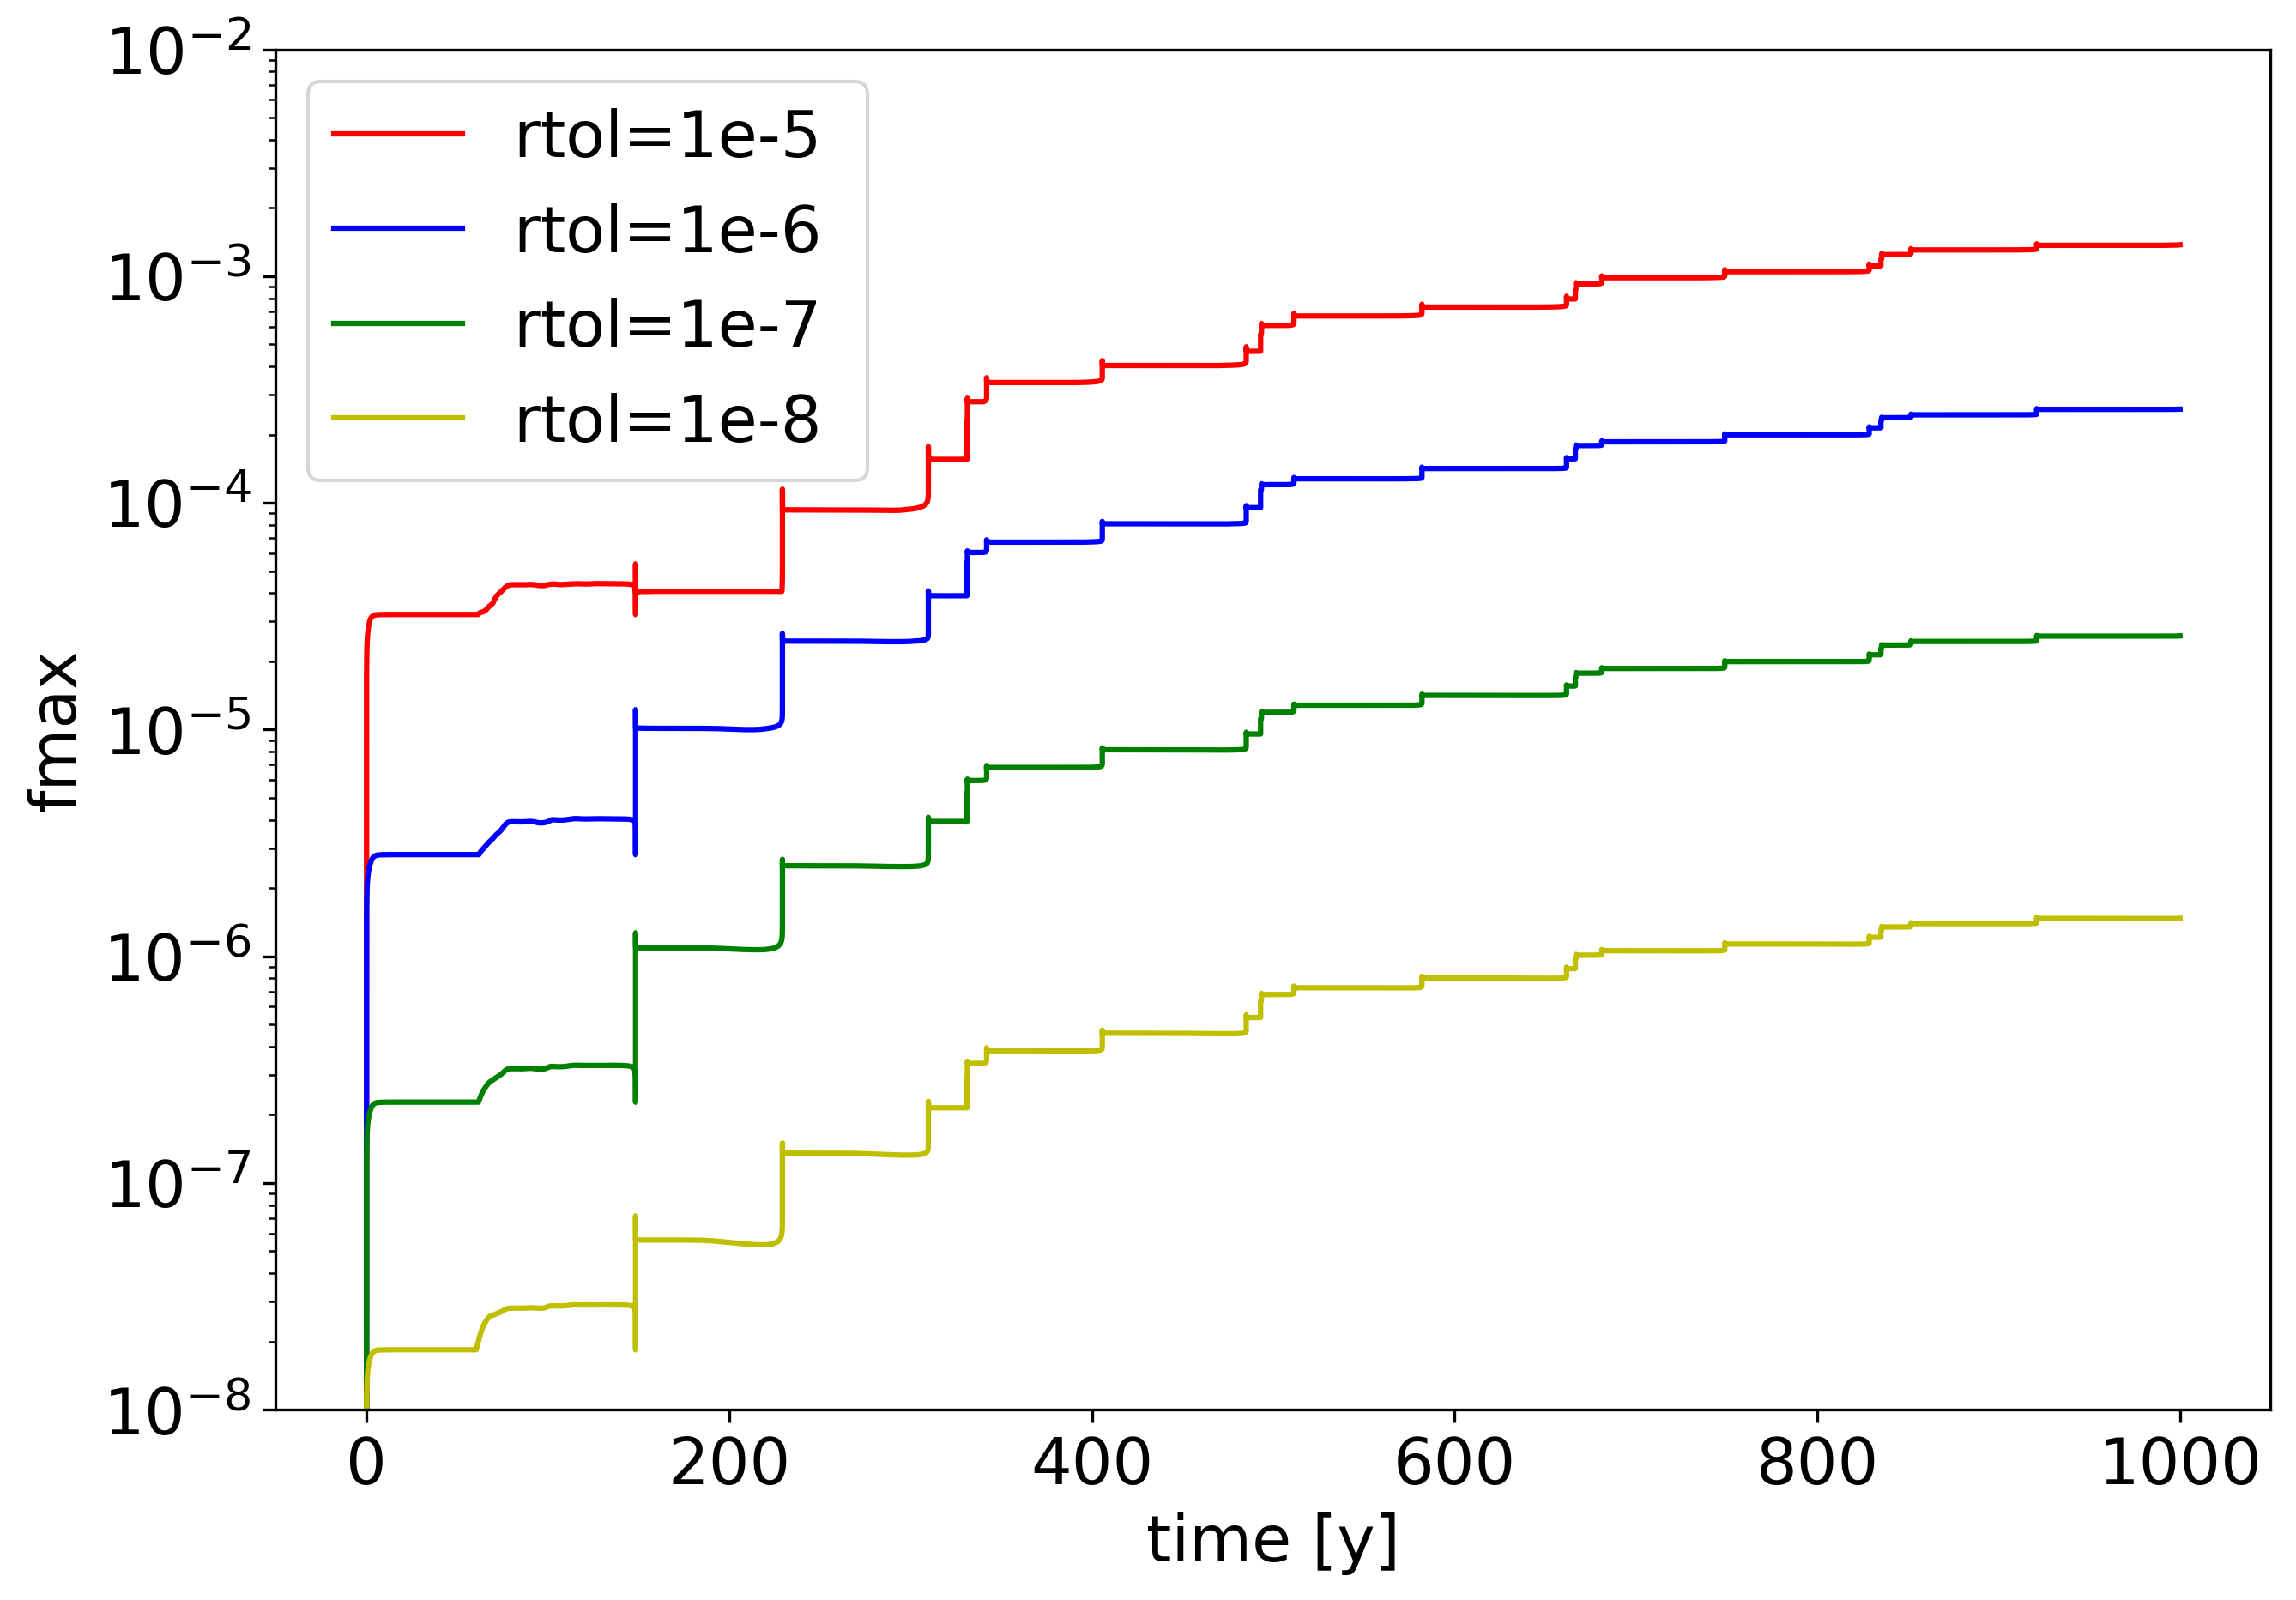
\includegraphics[width=1\textwidth]{images/TANDEMtimeEvolutionFExtendedODEDifferentTolerances.png}
		\subcaption{Maximum absolute value of the friction law} 
		\label{fig:timeEvolution_2ndOrderODE_differentTolerances}
	\end{subfigure}
	\begin{subfigure}{0.45\textwidth}
		\centering
		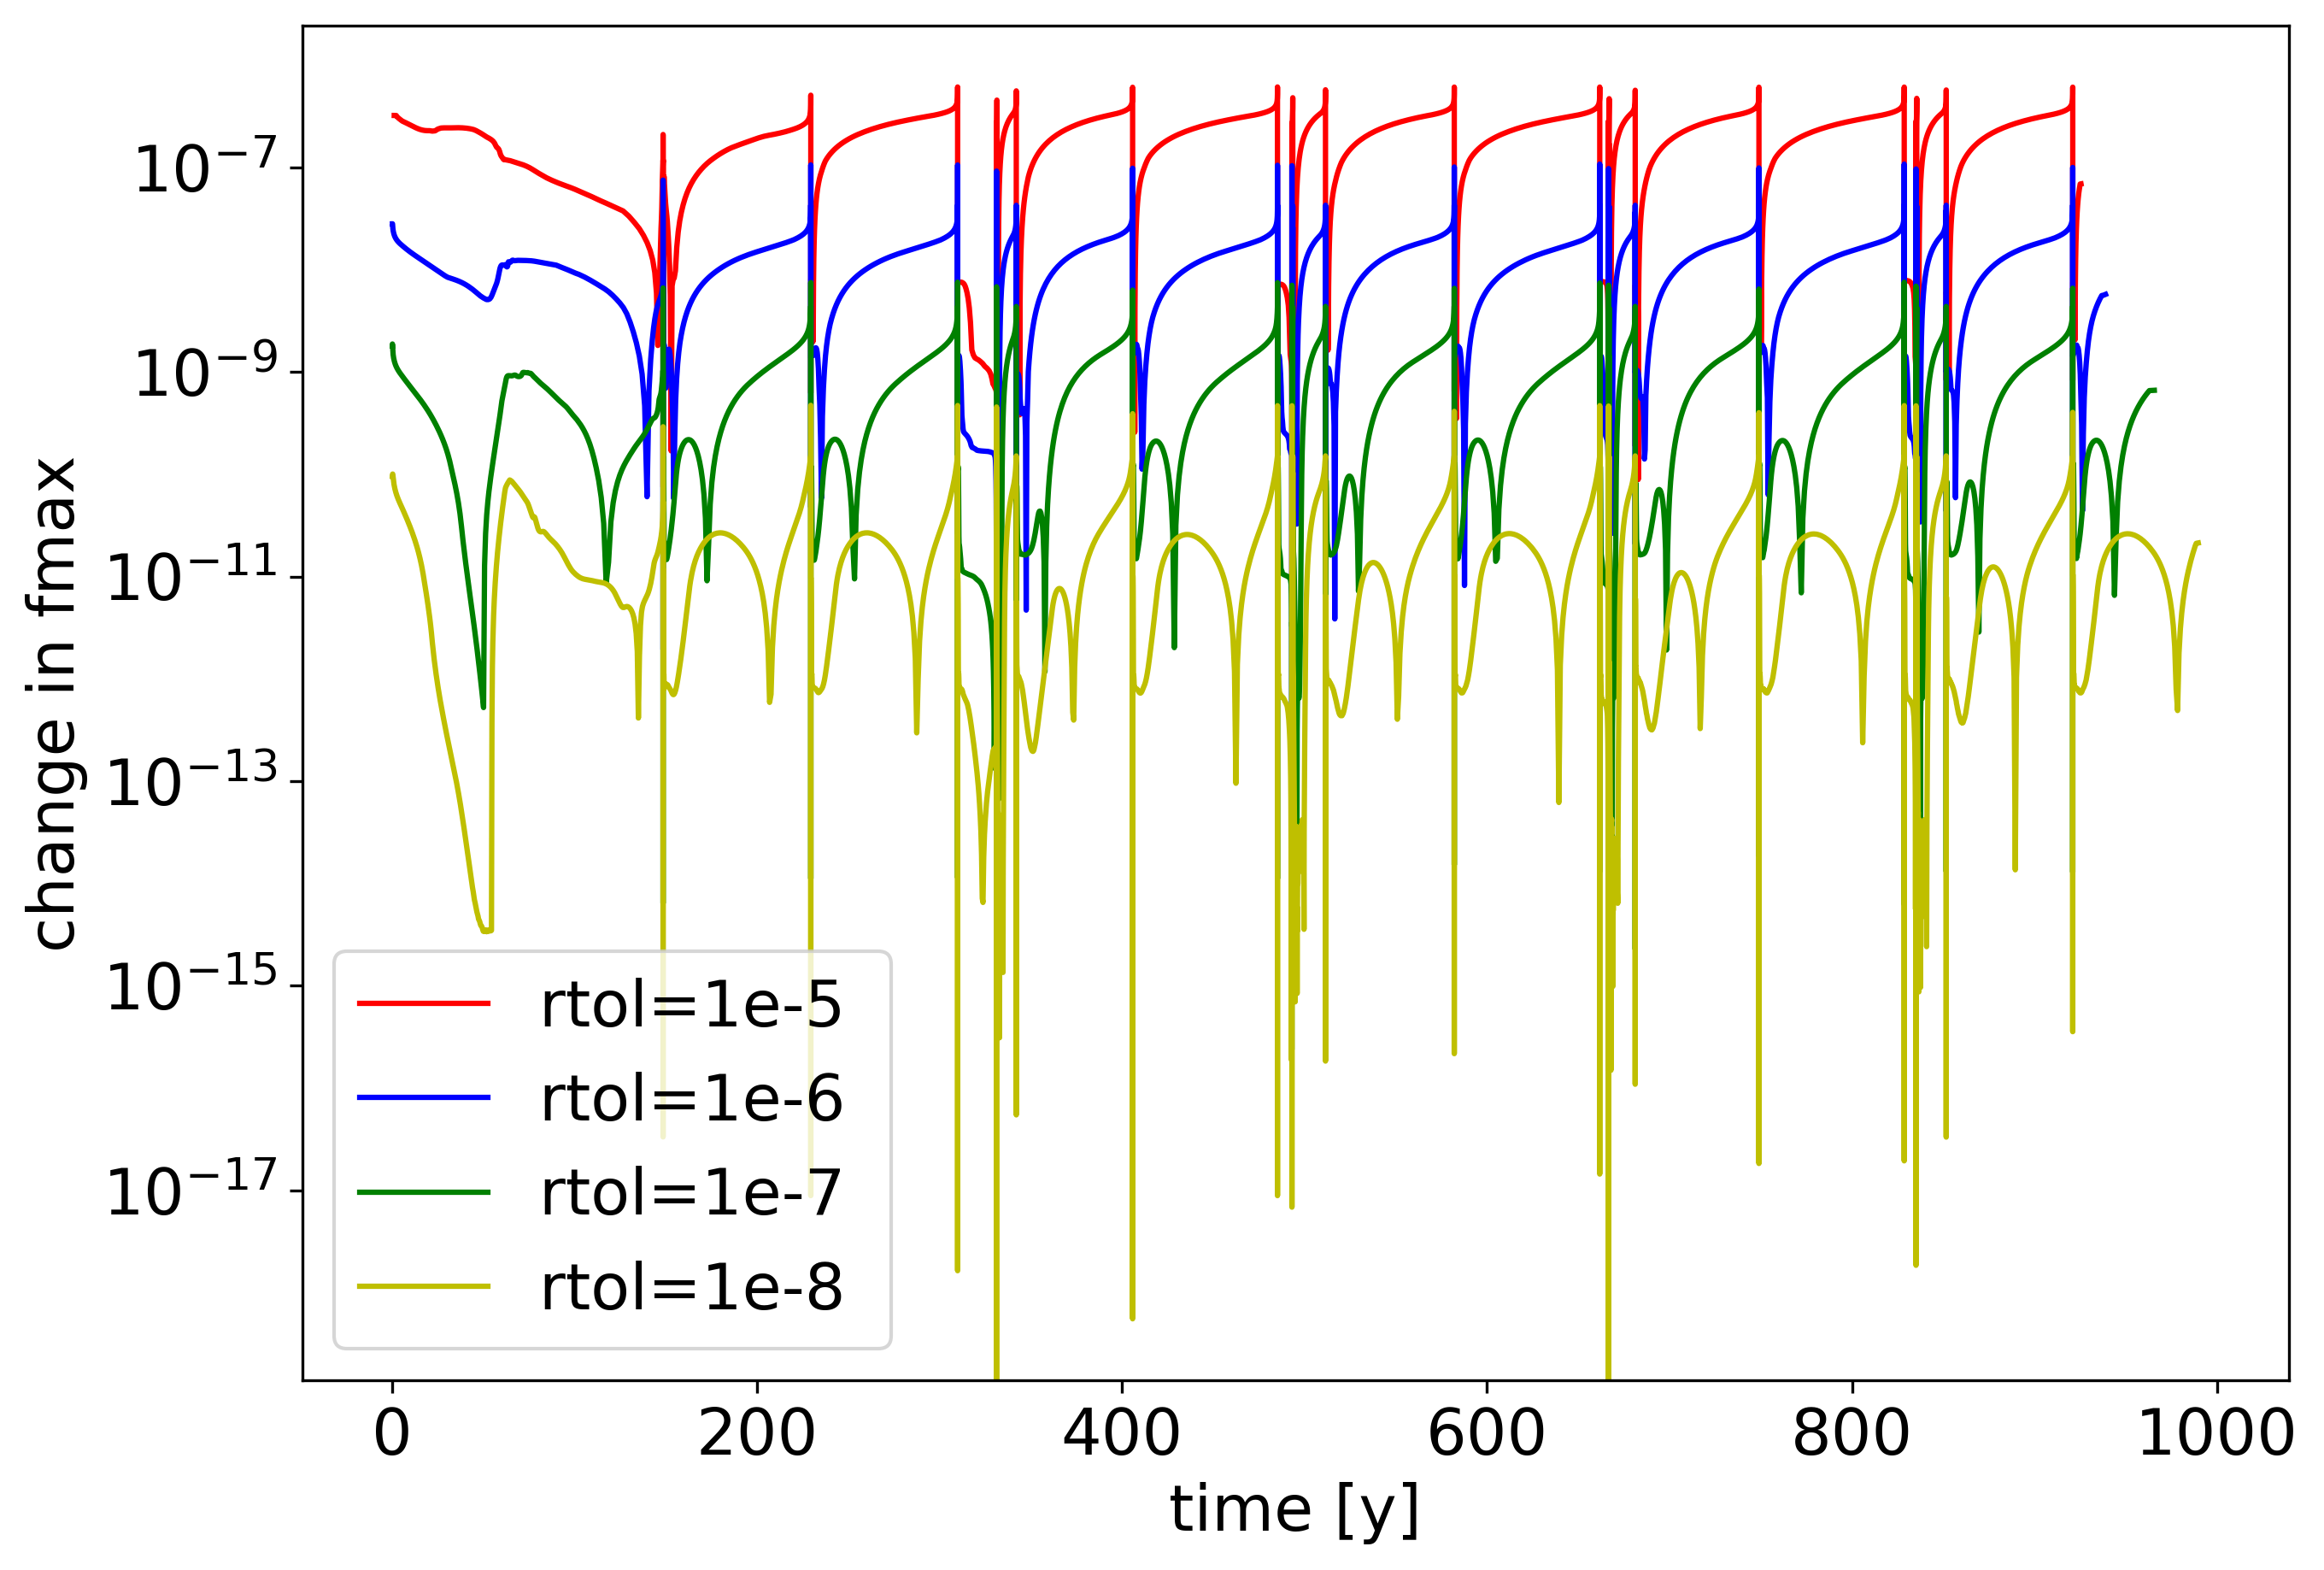
\includegraphics[width=1\textwidth]{images/TANDEMtimeEvolutionFLTEExtendedODEDifferentTolerances.png}
		\subcaption{Absolute change of the friciton law per timestep, averaged over 50 timesteps} 
		\label{fig:timeEvolution_LTE_2ndOrderODE_differentTolerances}
	\end{subfigure}
	\caption{Evolution of the value of the friction law of the 2nd order formulation with 5 elements on the fault over 1000 years with varying relative tolerances in the slip rate $V$}
\end{figure}

The local truncation error seems to depend linearly on the tolerance for the slip rate, and a similar dependency is to be expected with respect to the tolerances of the slip $S$ and $\psi$, since these quantities are also required to evaluate the friction law. Next, we investigate whether other parameters, such as the spatial discretization, have an effect on the global error too. For a fixed relative tolerance for the slip of $10^{-7}$, the simulation has been executed for different spatial resolutions and the evolution of the friction law in each case is shown in \autoref{fig:timeEvolution_2ndOrderODE_differentSizes}. Since each fault elements contains three fault nodes, one has to multiply $n$ by three to obtain the total number of simulated fault nodes. At the beginning, all domain sizes have a similar accuracy, but after some earthquakes, it seems that the error in domains with higher resolution increases less fast. However, in \autoref{fig:timeEvolution_LTE_2ndOrderODE_differentSizes}, it is hard to distinguish separate upper bounds for the local truncation error with different domain sizes. The better performance of larger domains is rather due to the overall higher accuracy of simulations with higher resolutions and to a lower incidence of earthquakes, than due to a reduction of the LTE. 

\begin{figure}[H]
	\centering
	\begin{subfigure}{0.45\textwidth}
		\centering
		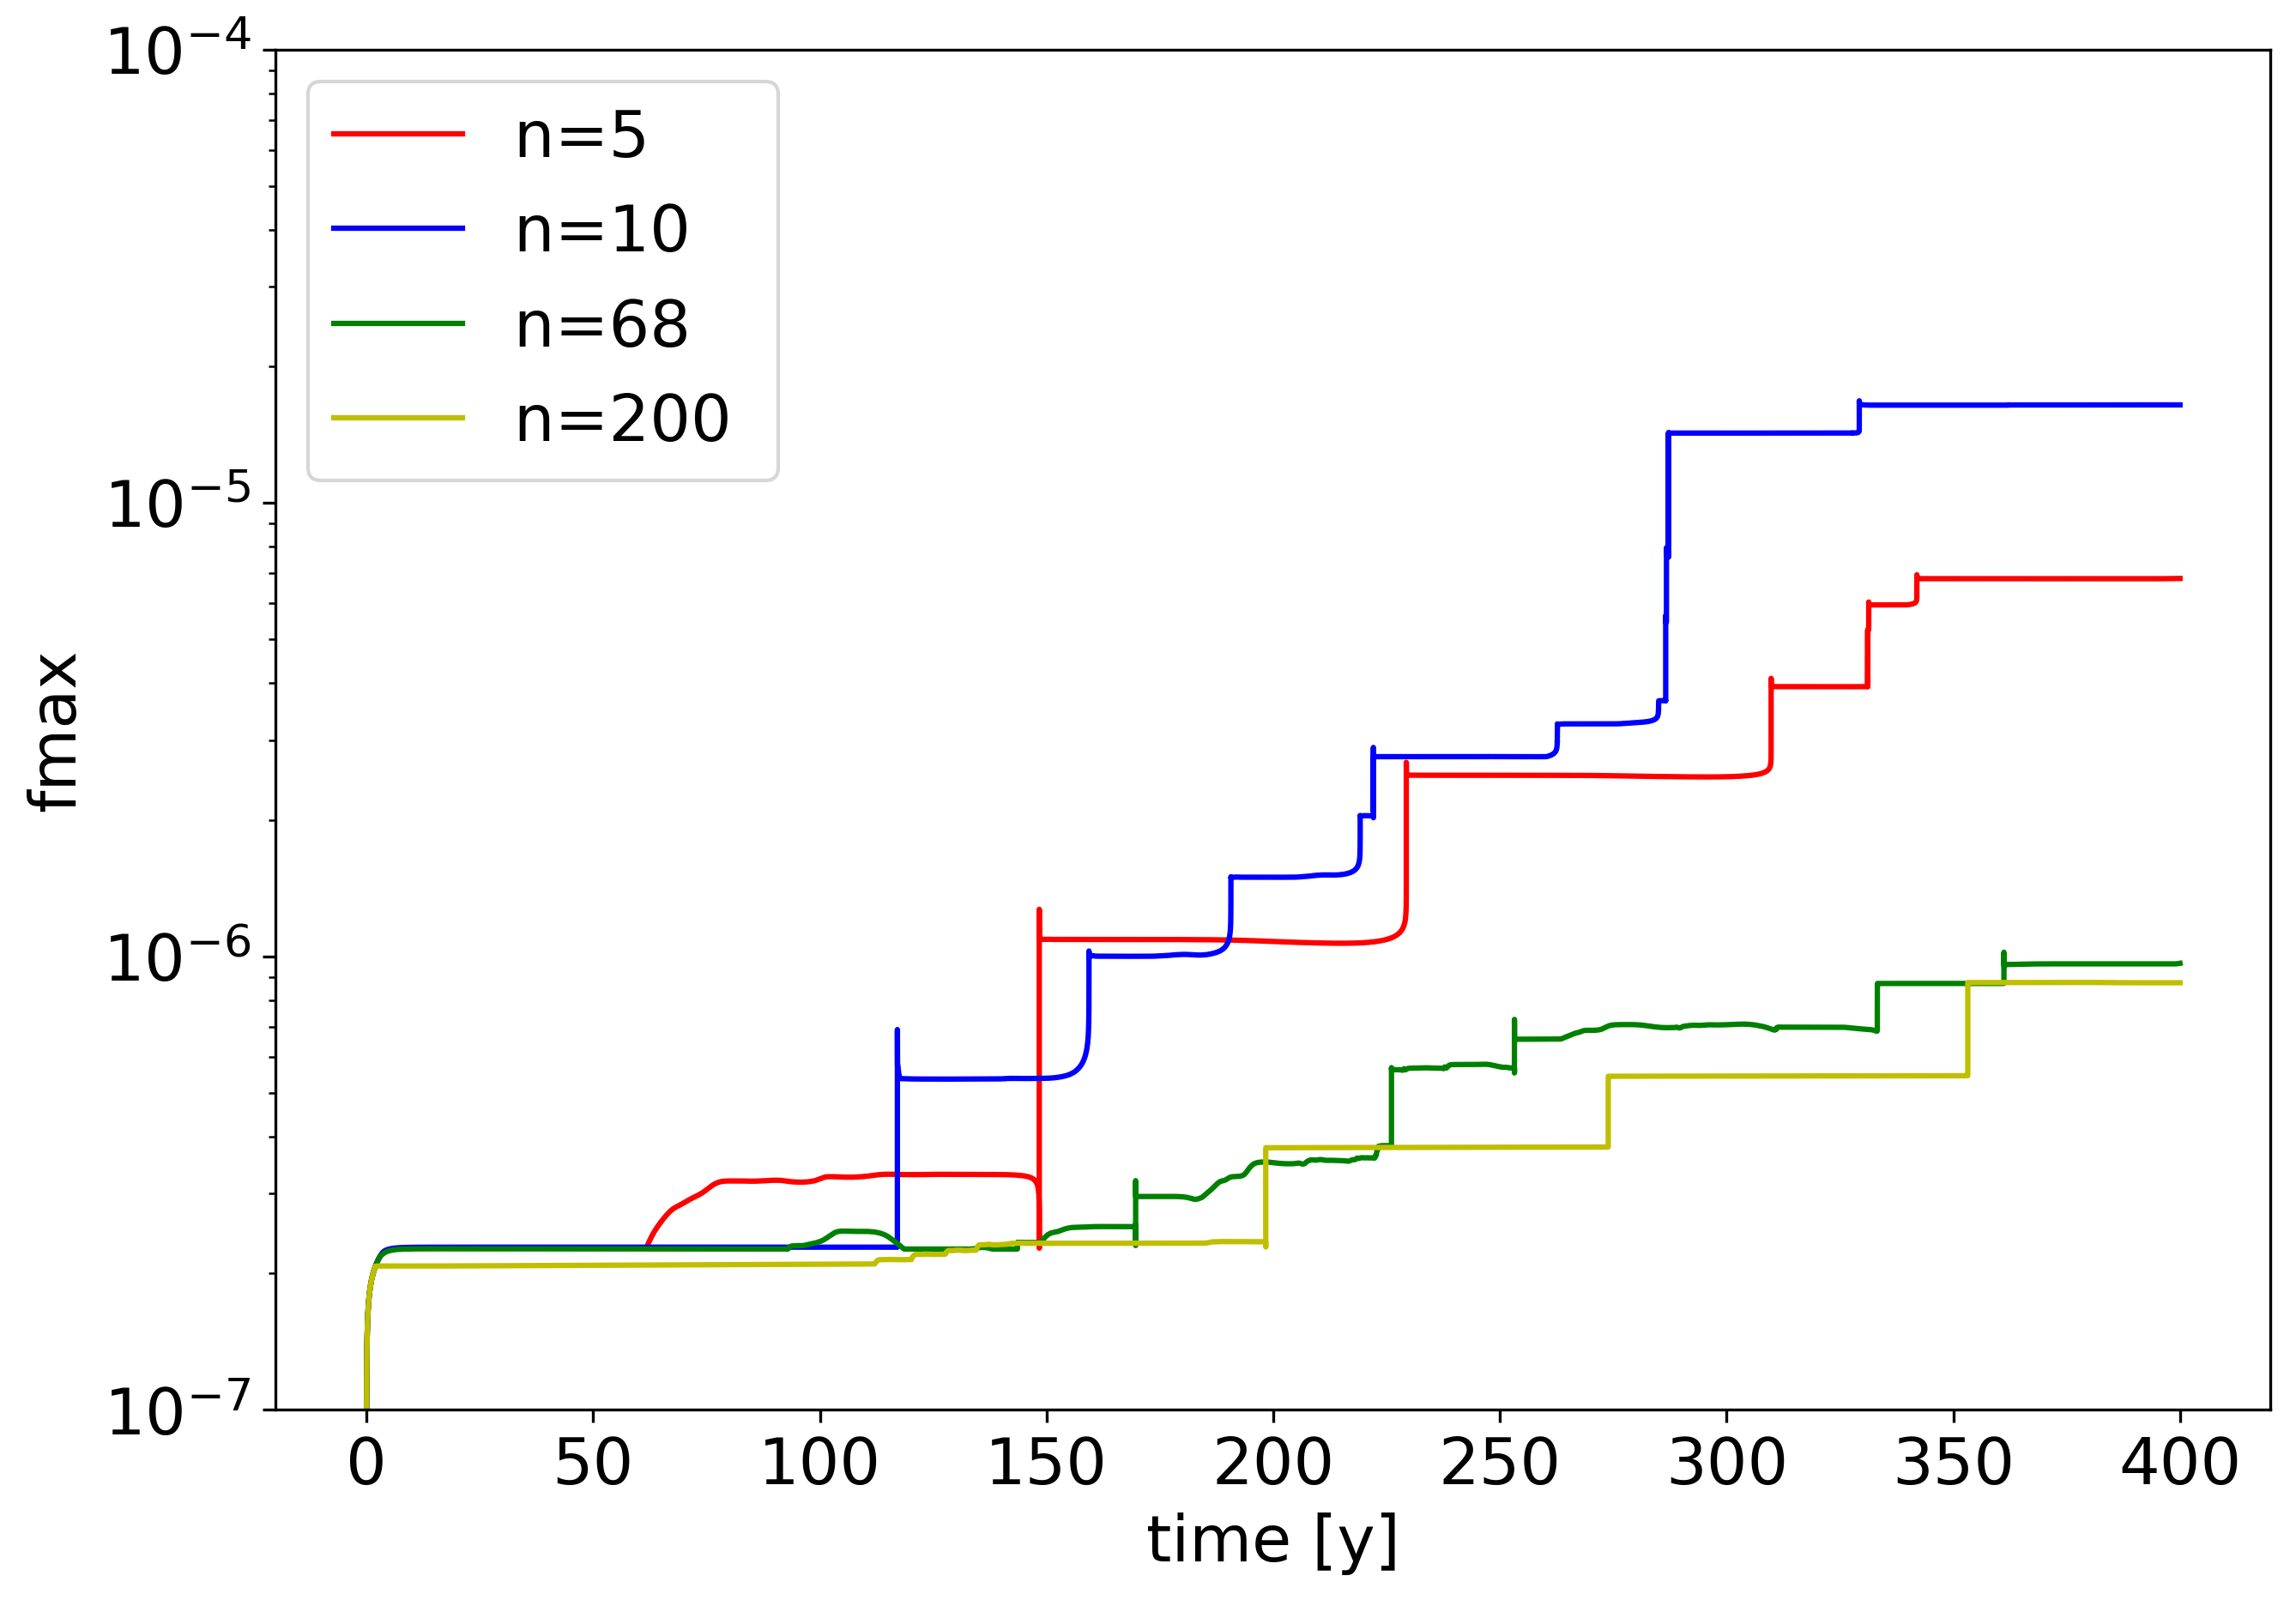
\includegraphics[width=1\textwidth]{images/TANDEMtimeEvolutionFExtendedODEDifferentSizes.png}
		\subcaption{Maximum absolute value of the friction law} 
		\label{fig:timeEvolution_2ndOrderODE_differentSizes}
	\end{subfigure}
	\begin{subfigure}{0.45\textwidth}
		\centering
		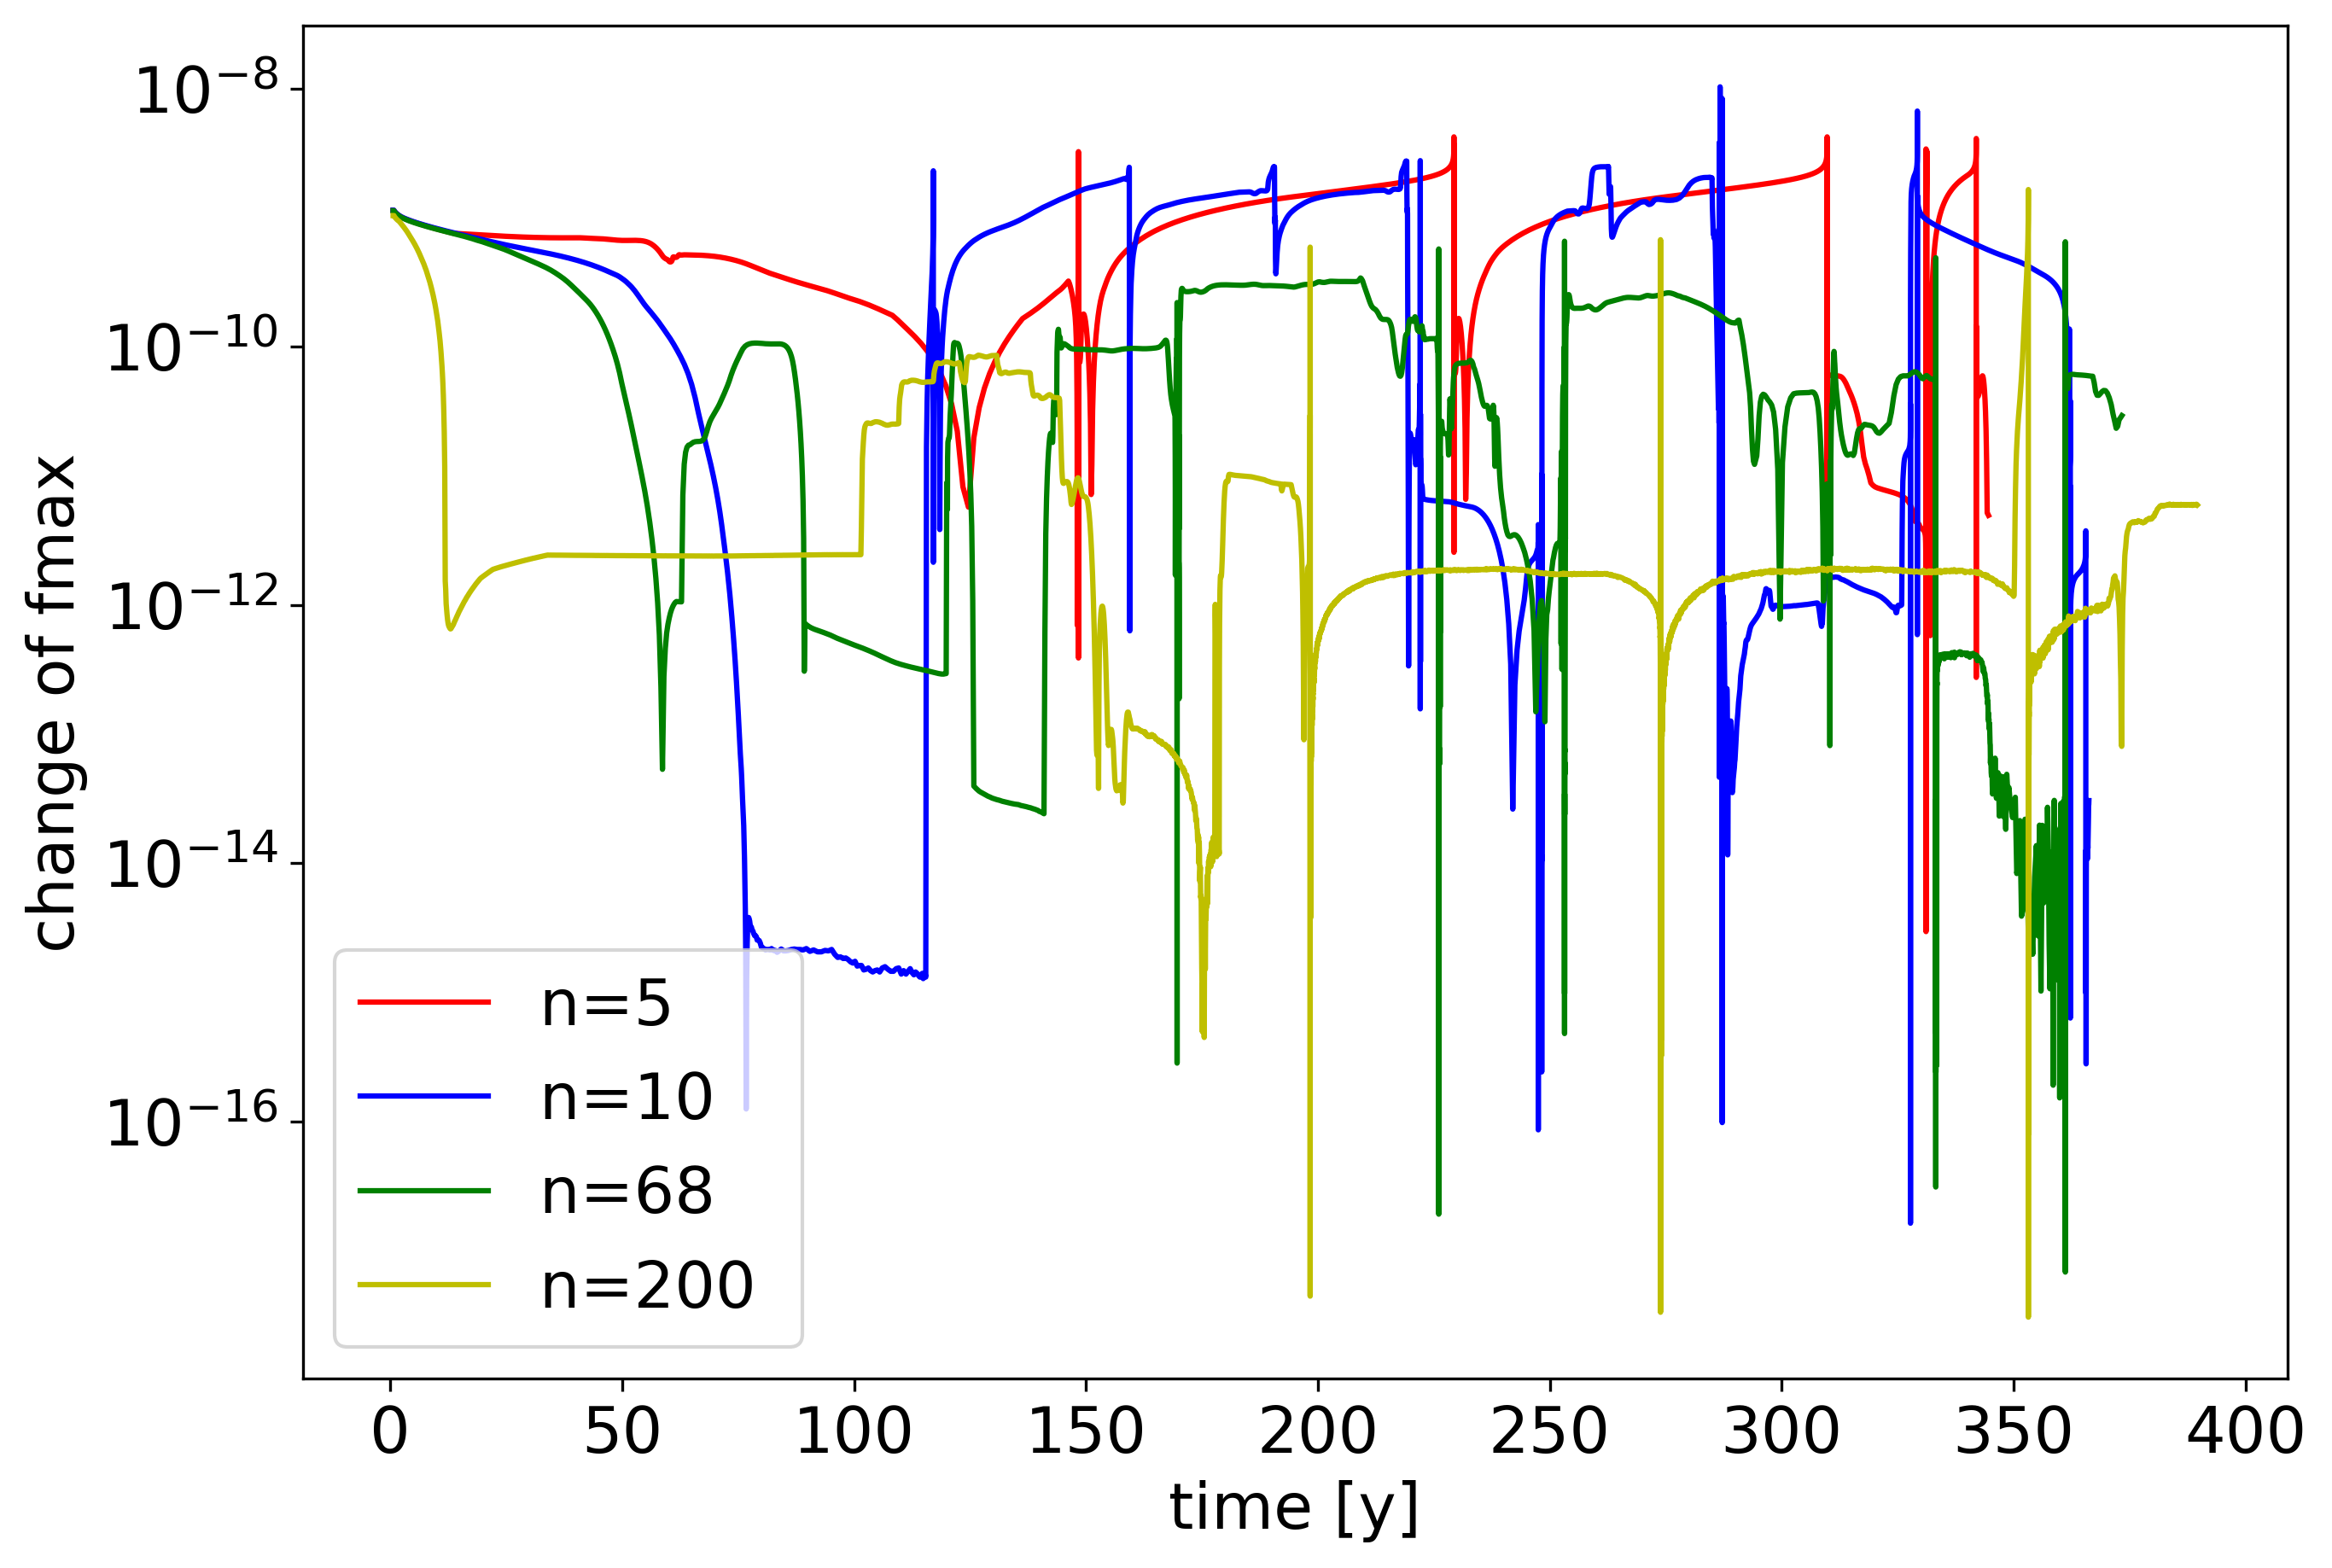
\includegraphics[width=1\textwidth]{images/TANDEMtimeEvolutionFLTEExtendedODEDifferentSizes.png}
		\subcaption{Absolute change of the friciton law per timestep, averaged over 50 timesteps} 
		\label{fig:timeEvolution_LTE_2ndOrderODE_differentSizes}
	\end{subfigure}
	\caption{Evolution of the value of the friction law of the 2nd order formulation over 400 years with varying domain sizes, where $n$ denotes the number of fault elements}
\end{figure}

Overall, the evaluation of the friction law is a suitable estimate for the global error in the system. Over the course of time, its value increases step wise at each earthquake, but overall linearly, which is due to a regular local truncation error. The main driver of the LTE is the tolerance for the slip rate $V$, which has been introduced to the system along with the second order ODE formulation. The upper bound for the LTE is proportional to the chosen tolerance.


\section{Time adaptivity of BDF methods}
\label{sec:Results_BDFOrder}
\subsection{Quality of the error estimates}
Two error estimates have been introduced for the BDF methods. For the embedded method, at each time step, a BDF scheme with higher order is applied to the current solution vector and the difference between both available solutions at the timestep yields the error estimate. The second method bases on the derivatives of Lagrangian polynomials as described in \autoref{sssec:errorEstimateBDFLagrange}, and has the advantage to be much cheaper to evaluate, since it does not require to solve the system again. It has already been shown in \autoref{ssec:QualityErrorEstimate_0D} that for the 0D example, the first method gives a more accurate estimation of the local truncation error than the second method. Both methods tend to overestimate the error, which is for sure a safe behavior, but restrict the choice of the next timestep. Since here no exact solution is available for any physical quantity, the accuracy of the error estimate cannot be directly determined as previously. Instead, we assume that the actual error is inferior to the estimate, and that the embedded method is more accurate than Lagrangian polynomials. We would then expect the timestep adapter to choose larger timesteps with the first method and finish the program earlier. The aim of this section is to see, whether the more accurate embedded method allows for larger timesteps than the error estimate with Lagrangian polynomials, and if so, whether the total number of timesteps can be reduced enough to justify the higher costs of the embedded method. \\
The first assumption is verified in \autoref{fig:BDFOrders_Lagrange_vs_Embedded_extended_DAE} for the extended DAE formulation. As expected, the embedded method is faster than Lagrangian polynomials, as features of the curve, such as an increase or decrease of the timestep size happen increasingly earlier with the embedded method. Overall, fewer timesteps are required to reach a solution at a given time. However, the allowed timesteps are only slightly larger and the difference cannot be noticed on the logarithmic scale. Nonetheless, it is positive to remark that the same small features such as intermediate peaks are observed with both methods, which indicates that both error estimates recognize the same inconsistencies in the solution. 
\begin{figure}[H]
	\centering
	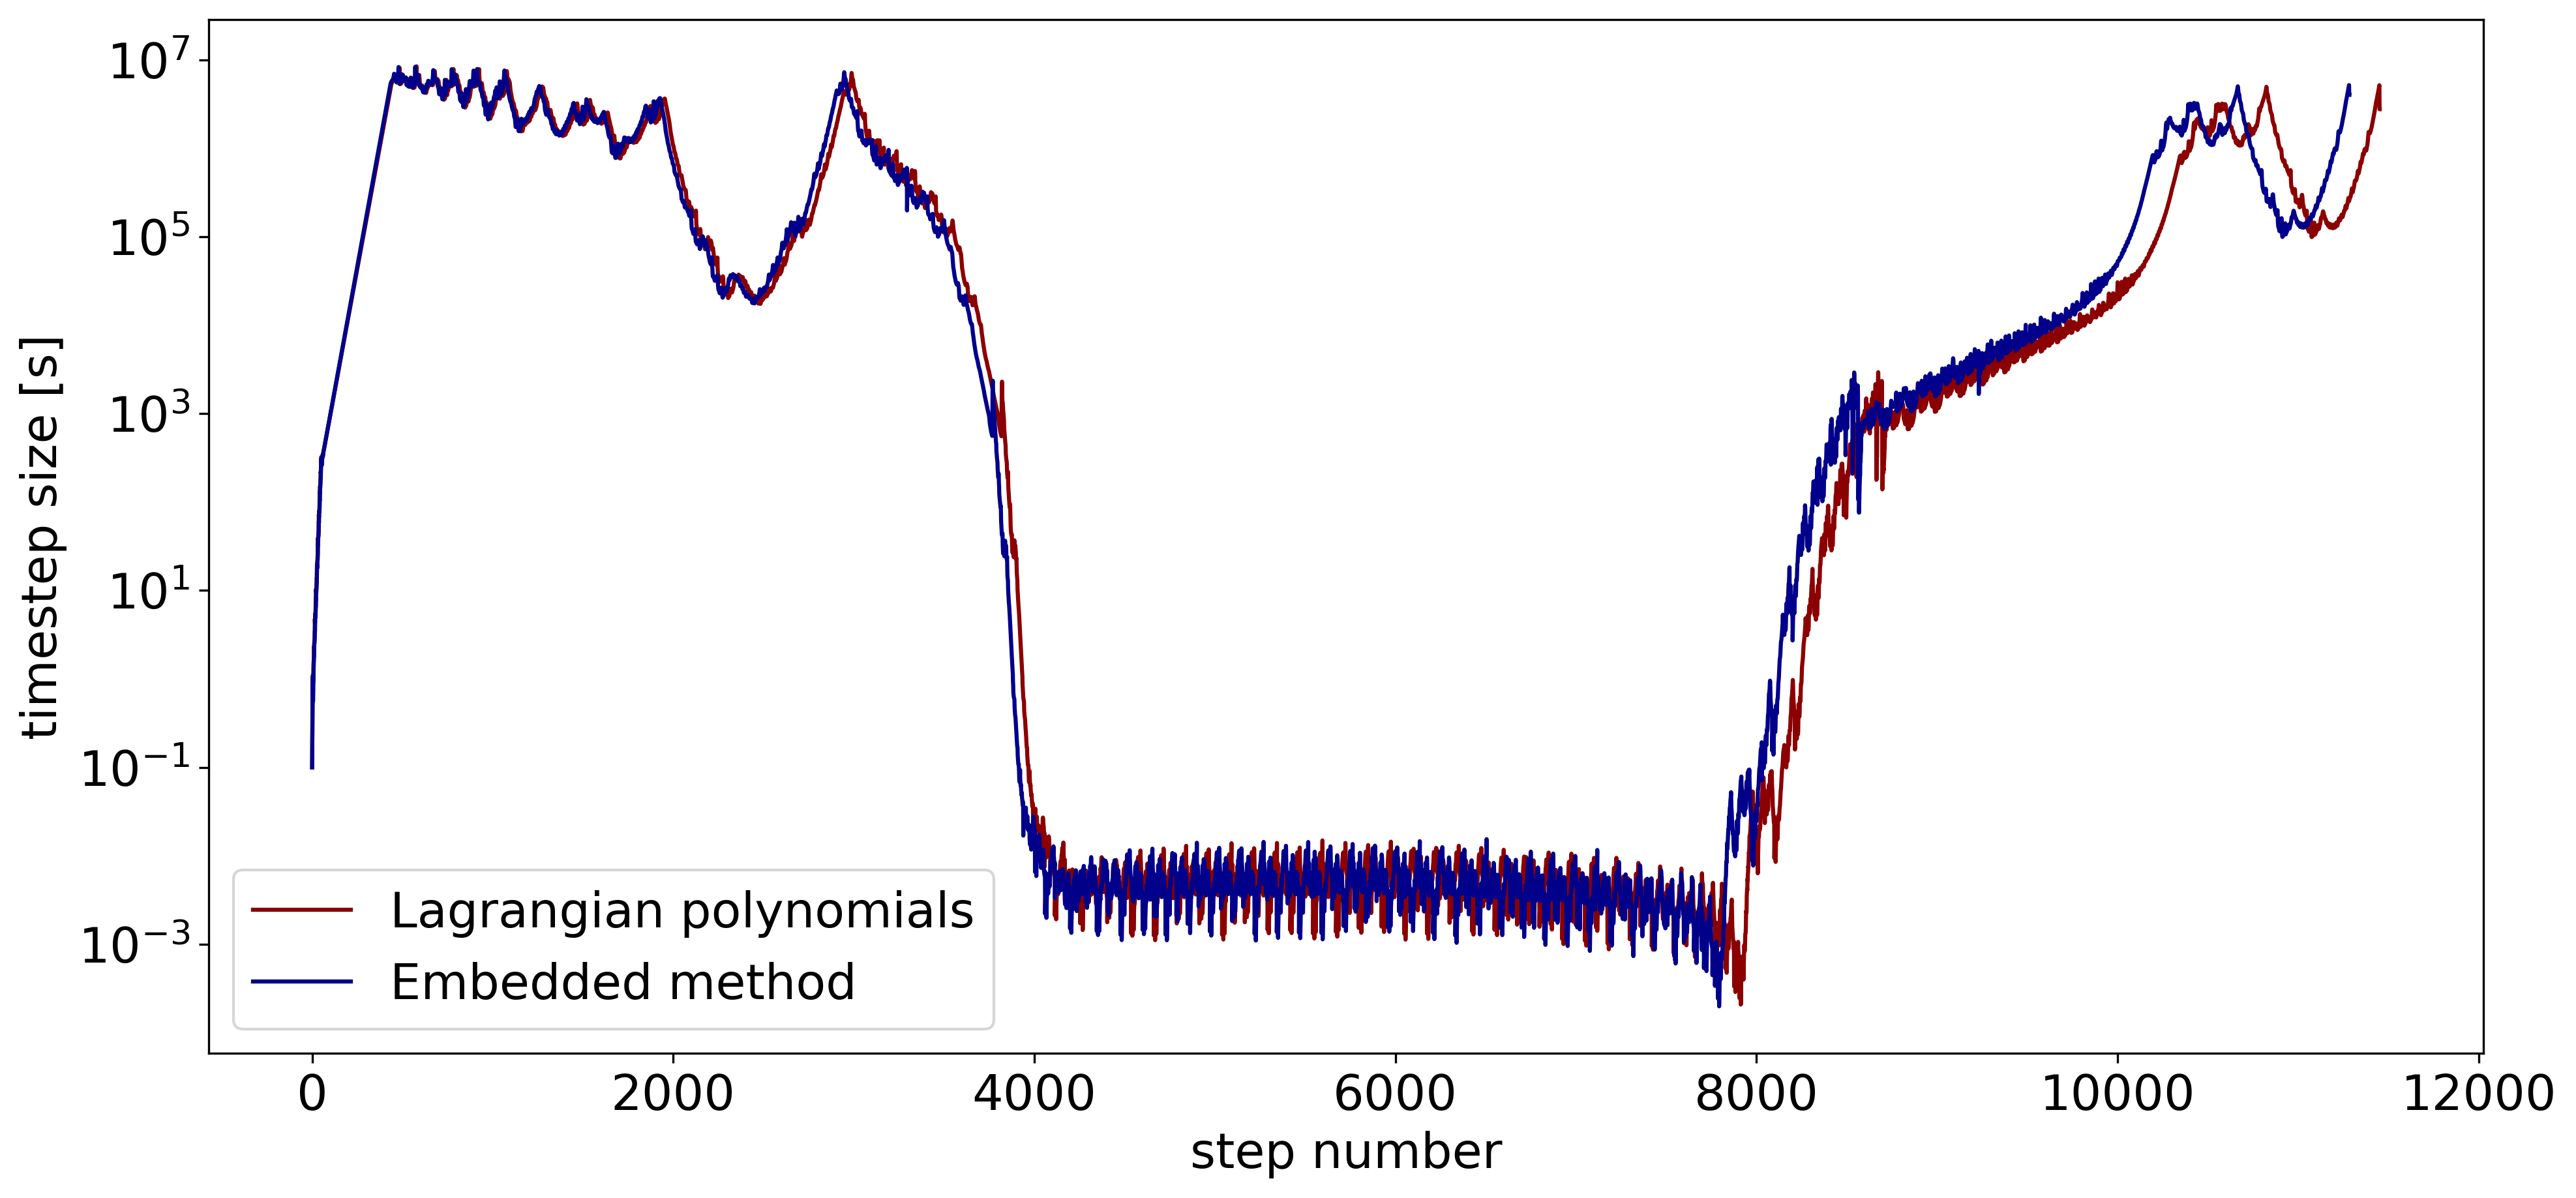
\includegraphics[width=0.8\textwidth]{images/TANDEMTimeAnalysisDifferentBDFOrdersEmbedded_vs_Lagrange_ExtendedDAE_Size101.png}
	\caption{Comparison of the chosen timestep sizes with the error estimates by Lagrangian polynomials and by an embedded method with a 5th order BDF method on a domain with 101 fault elements using the extended DAE formulation. }
	\label{fig:BDFOrders_Lagrange_vs_Embedded_extended_DAE}
\end{figure}
Overall, the embedded method gives a more accurate error estimate than the Lagrangian polynomials, and allows for larger timestep sizes. However, the gain is only very small, as in average 2\% fewer timesteps are required at the end of the simulation, and this does not justify the use of the embedded higher order BDF method as error estimate, as it is twice as expensive. Actually, the order of the BDF method has a much higher influence on the total number of iterations, as it will be discussed in the following section.


\subsection{Effect of the order on the timestep size}
The simulation can be roughly split into four sections: the evolution of the aseismic slip, with an approximately constant stepsize of the order of $h=10^6$s, the evolution of the earthquake at $h=10^{-2}$s and the transition between both phases, where the stepsize progressively increases or decreases. In addition to that, there is the initialization phase, in which the stepsize starts at $h=0.1$s to quickly reach the stepsize of the aseismic slip. \\
The transition from the aseismic slip to the earthquake is a crucial section, because the sudden increase of the slip rate requires to rapidly scale down the timestep size. The end of the earthquake is less critical, as the slip rate drops relatively slowly which gives more scope to the stepsize to adapt to it, moreover the eventual too small stepsize there is not as problematic as a too high stepsize at the beginning of the earthquake. It is also interesting to look at the initialization phase, as there are no other constraints for a small stepsize but the limitations of the BDF scheme. In this section, we investigate the ability of BDF schemes of different orders to rapidly scale the timesteps size up or down. \\
\autoref{fig:BDFOrders_extended_DAE_compare_initialization} shows the increase at the beginning of the simulation for the BDF methods of order 3-6 and \autoref{fig:BDFOrders_extended_DAE_compare_begin_first_EQ} shows the transition from the aseismic slip to the first earthquake. In the initialization phase, the slope is in general steeper if a higher order method is used. One notable exception is the 6th order BDF scheme, which has a lower slope than expected. Unlike the other schemes, it does not increase smoothly but has regular steps, which indicates that the 6th order scheme is not as stable as the others. It seems that it first tries to increase the timestep size by a large factor, but has to correct it down after a few steps again because the error tolerance is not respected. Overall, the increase is perfectly exponential for the schemes 3-5, and the factor by which the timestep size increases at each step is driven by the order of the method. Interestingly enough, in the very first timesteps,  the timestep size of the 2nd order scheme jumps by two orders of magnitude whereas the 5th and 6th order do not benefit at all from such a strong initial increase. 

\begin{figure}[H]
	\centering
	\begin{subfigure}[b]{0.45\textwidth}
		\centering
		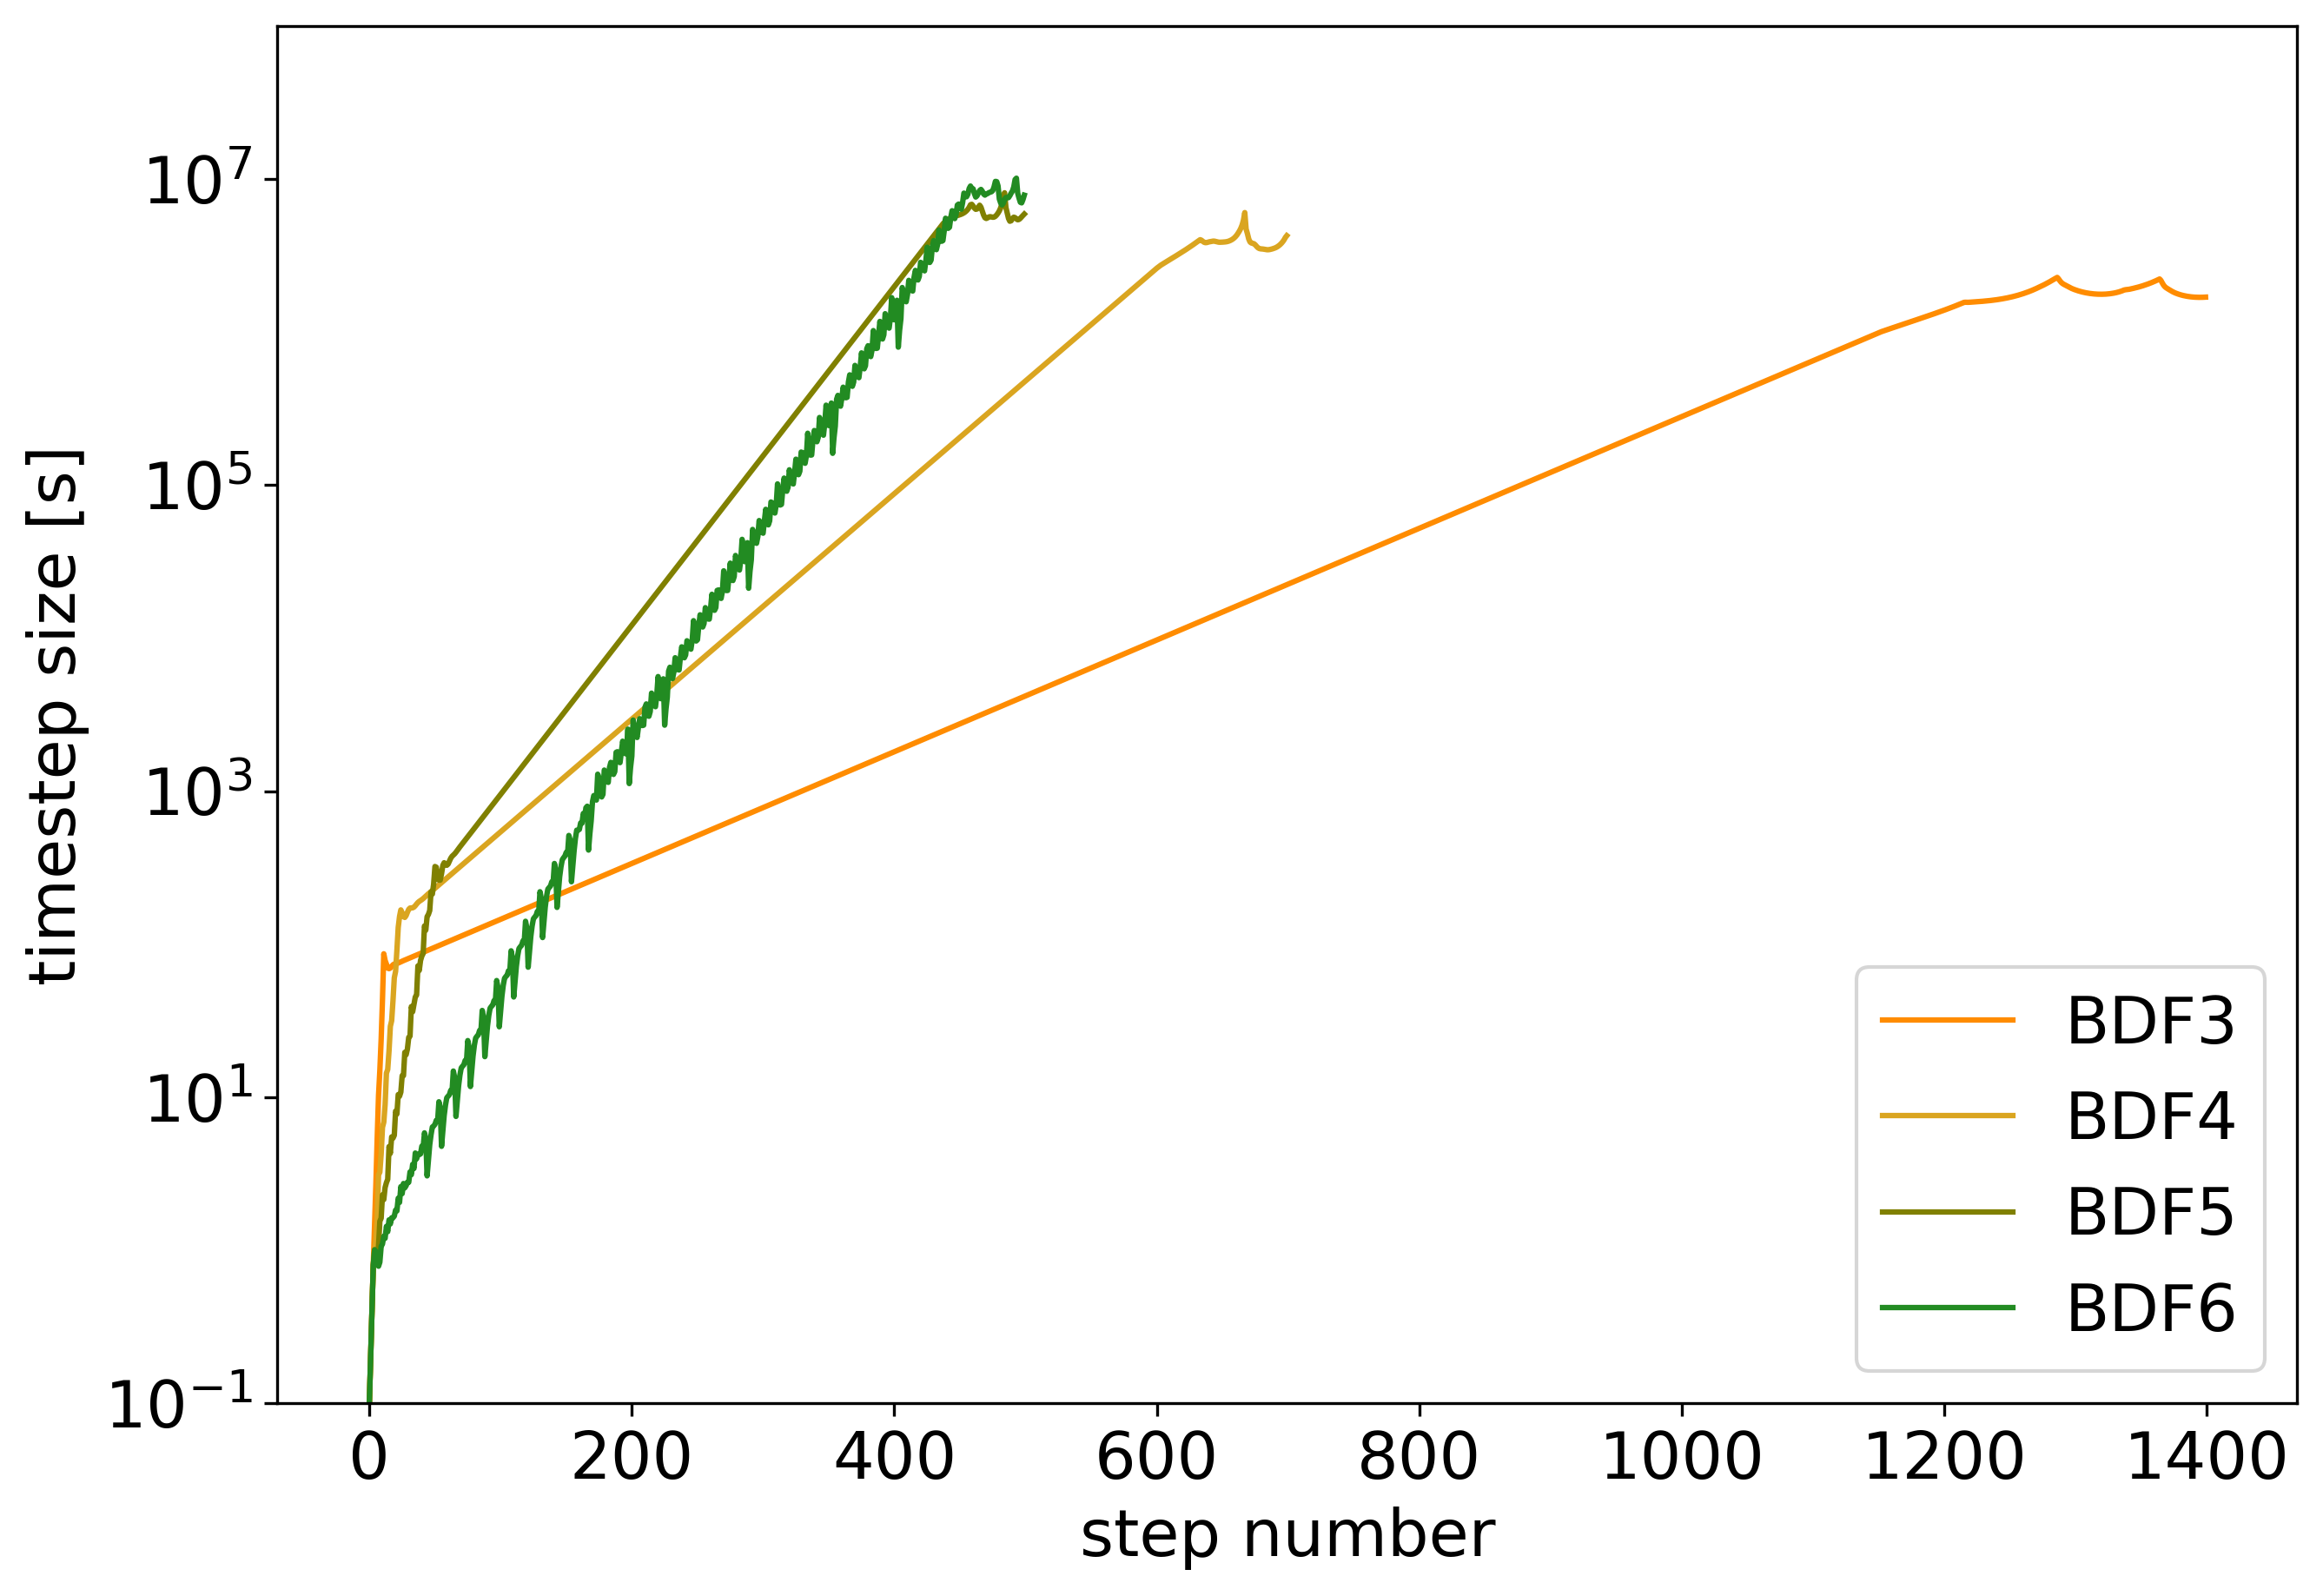
\includegraphics[width=1\textwidth]{images/TANDEMTimeAnalysisDifferentBDFOrdersLagrange_ExtendedDAE_Size101_Init.png}
		\subcaption{At the beginning of the simulation \\ \ } 
		\label{fig:BDFOrders_extended_DAE_compare_initialization}
	\end{subfigure}
	\begin{subfigure}[b]{0.45\textwidth}
		\centering
		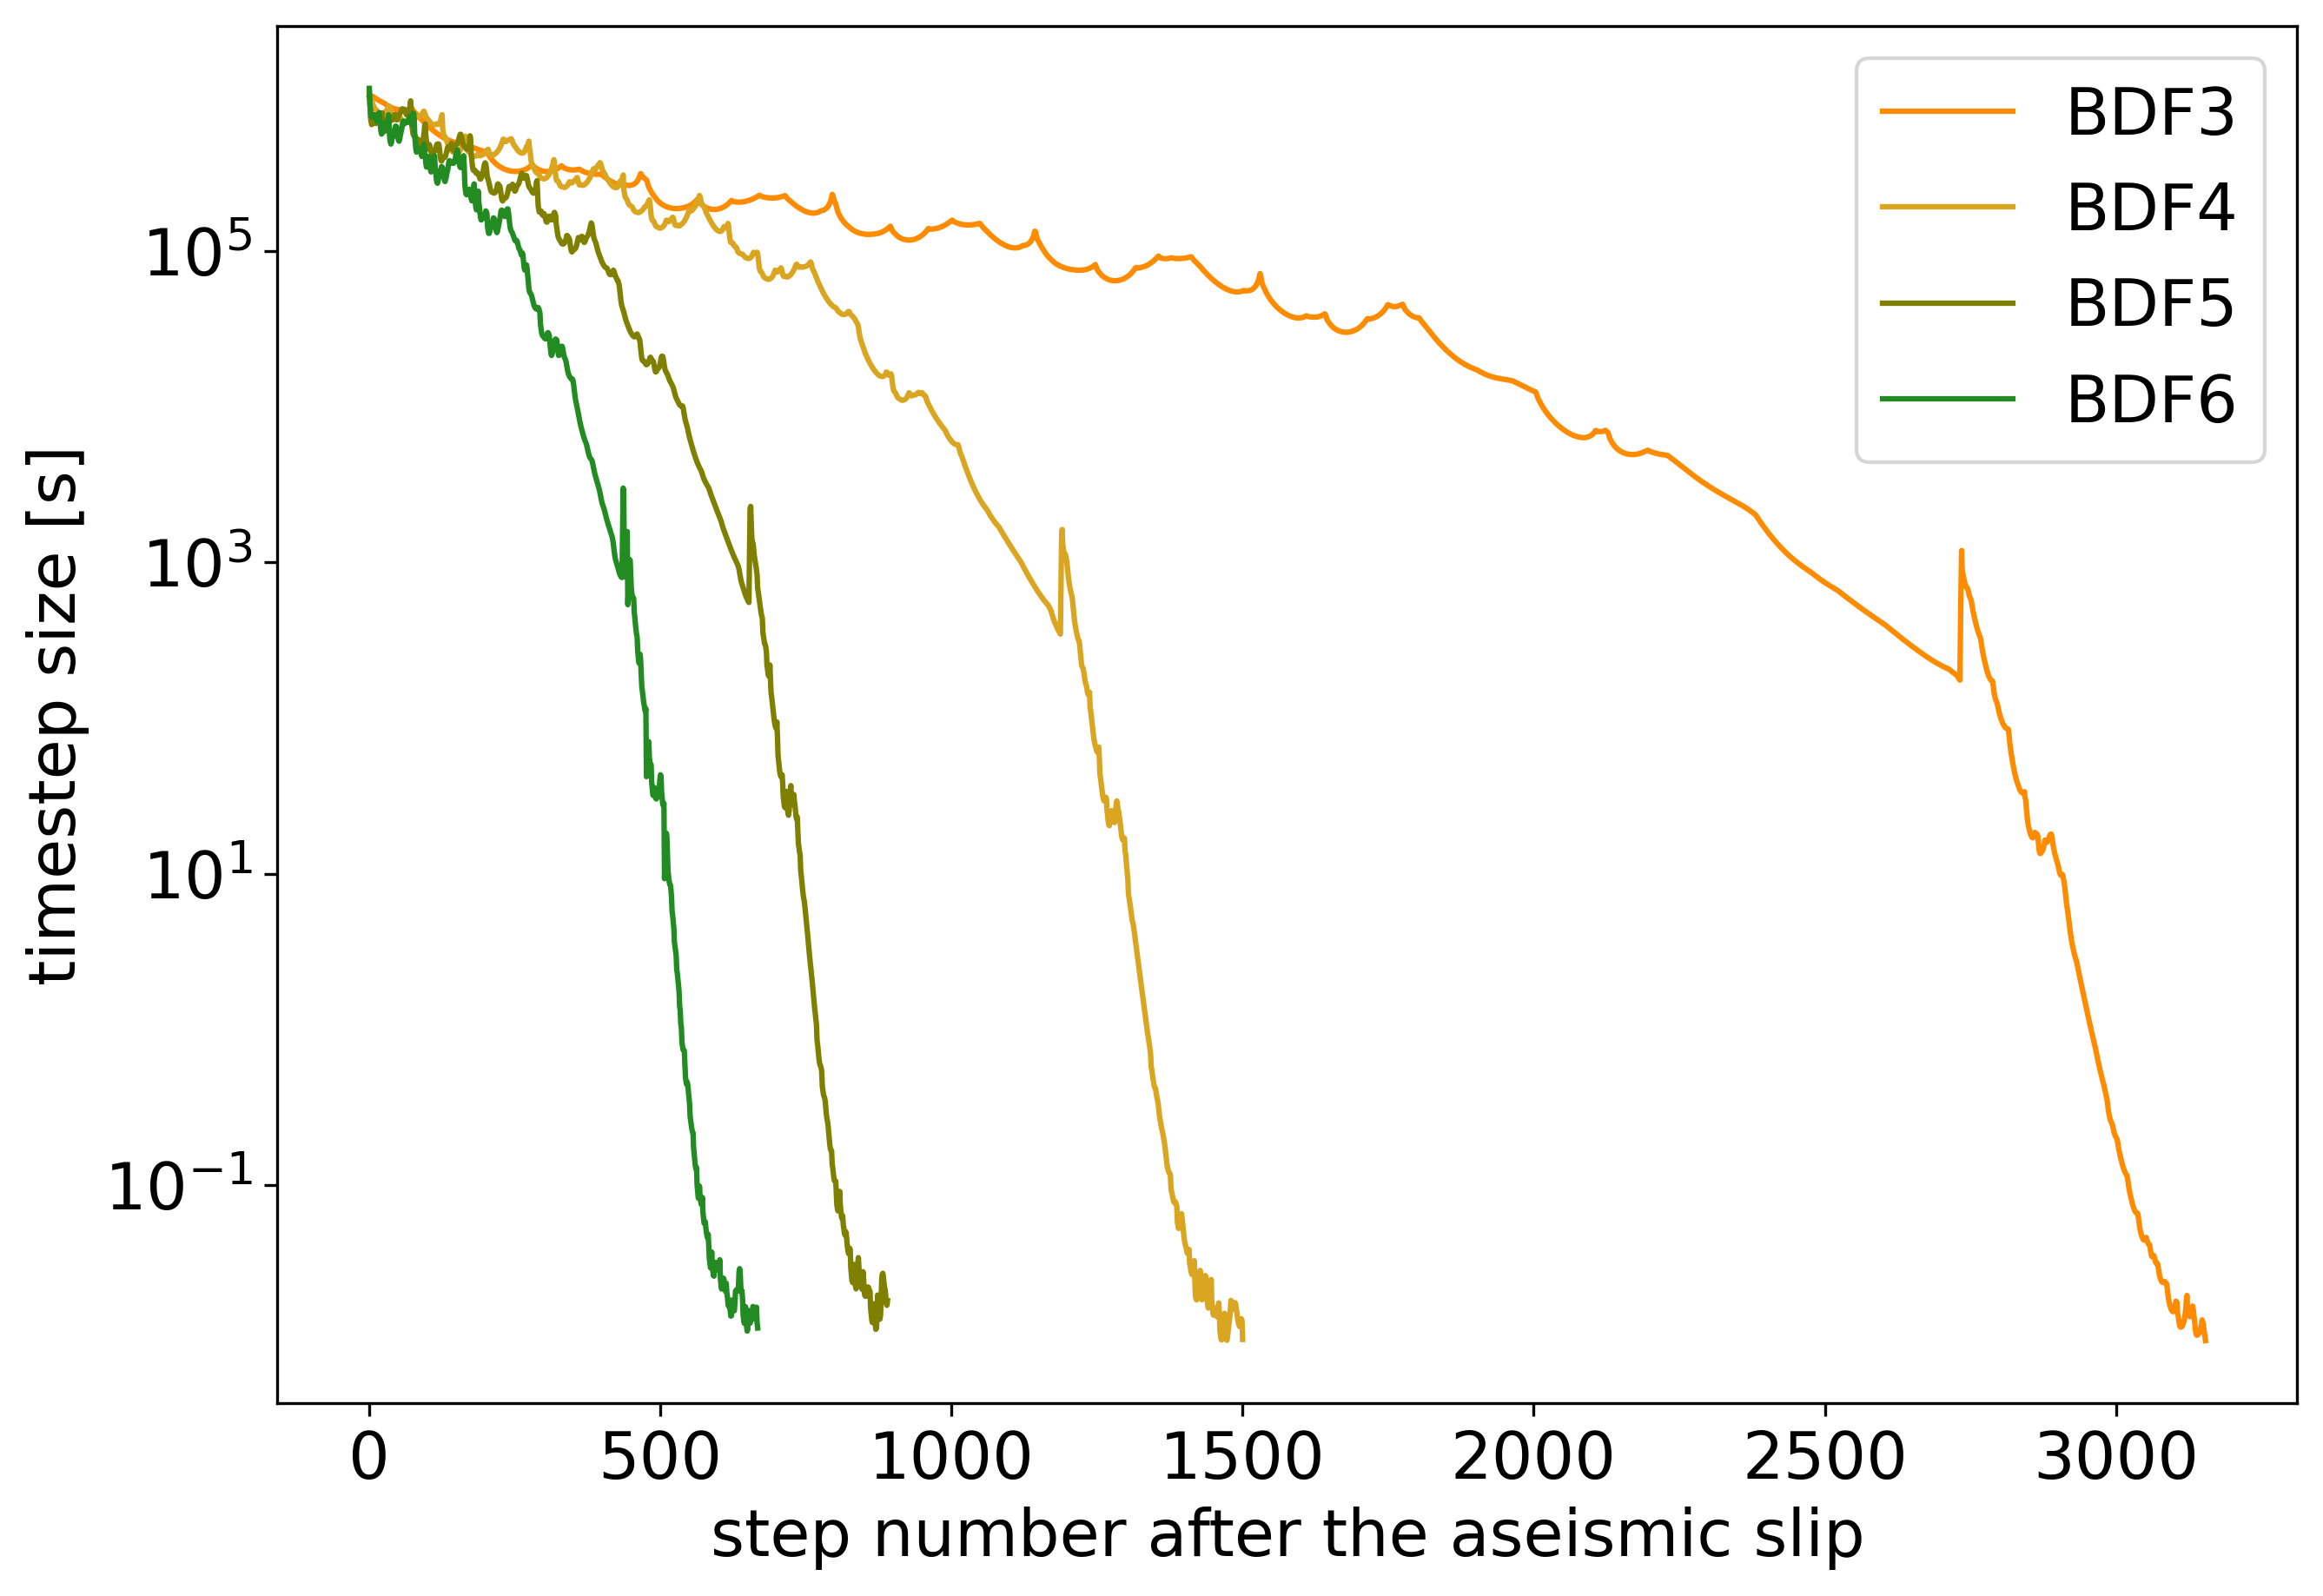
\includegraphics[width=1\textwidth]{images/TANDEMTimeAnalysisDifferentBDFOrdersLagrange_ExtendedDAE_Size101_Begin1stEQ.png}
		\subcaption{At the transistion from the aseismic to the earthquake phase}
		\label{fig:BDFOrders_extended_DAE_compare_begin_first_EQ}
	\end{subfigure}
	\caption{Evolution of the time step size for BDF schemes with different order at key points in the simulation on a domain with 101 fault elements using the extended DAE formulation}
\end{figure}

At the transition from the aseismic slip to the earthquake phase, the timestep size decreases exponentially with the same pattern: a higher order scheme allows a stronger reduction of the timestep size from one step to the next. Now, the 6th order scheme is perfectly stable and has the steepest slope among all BDF methods. \\


Higher order BDF methods allow in general for higher stepsizes and are to be preferred over lower order methods. Since the costs of all BDF schemes are similar (they converge similarly fast and each Newton step always requires to solve one linear system), there is no strong reason to prefer a low order scheme. Because of the stability issues with the 6th order scheme when the stepsize increases, the best performance can be expected from the 5th order scheme. There are some few cases where lower order methods perform better, such at the very beginning of the simulation. To take advantage of these peculiarities, and also to use the 6th order method if it is currently stable, the order of the BDF scheme can be adapted at each timestep as described in \autoref{sssec:adaptiveBDFOrder}. In this case, each step also calculates by how much the timestep size would change if one order higher or lower was used, and if a larger timestep can be reached, the order is changed accordingly for the next timestep. This has been implemented and the performance of the order-adaptive BDF scheme is shown in \autoref{fig:BDFOrders_extended_DAE_compare_adaptiveBDF}. It successfully uses the scheme with the largest allowable stepsize and finishes the simulation faster than any other methods, without any notable additional costs. 


\begin{figure}[H]
	\centering
	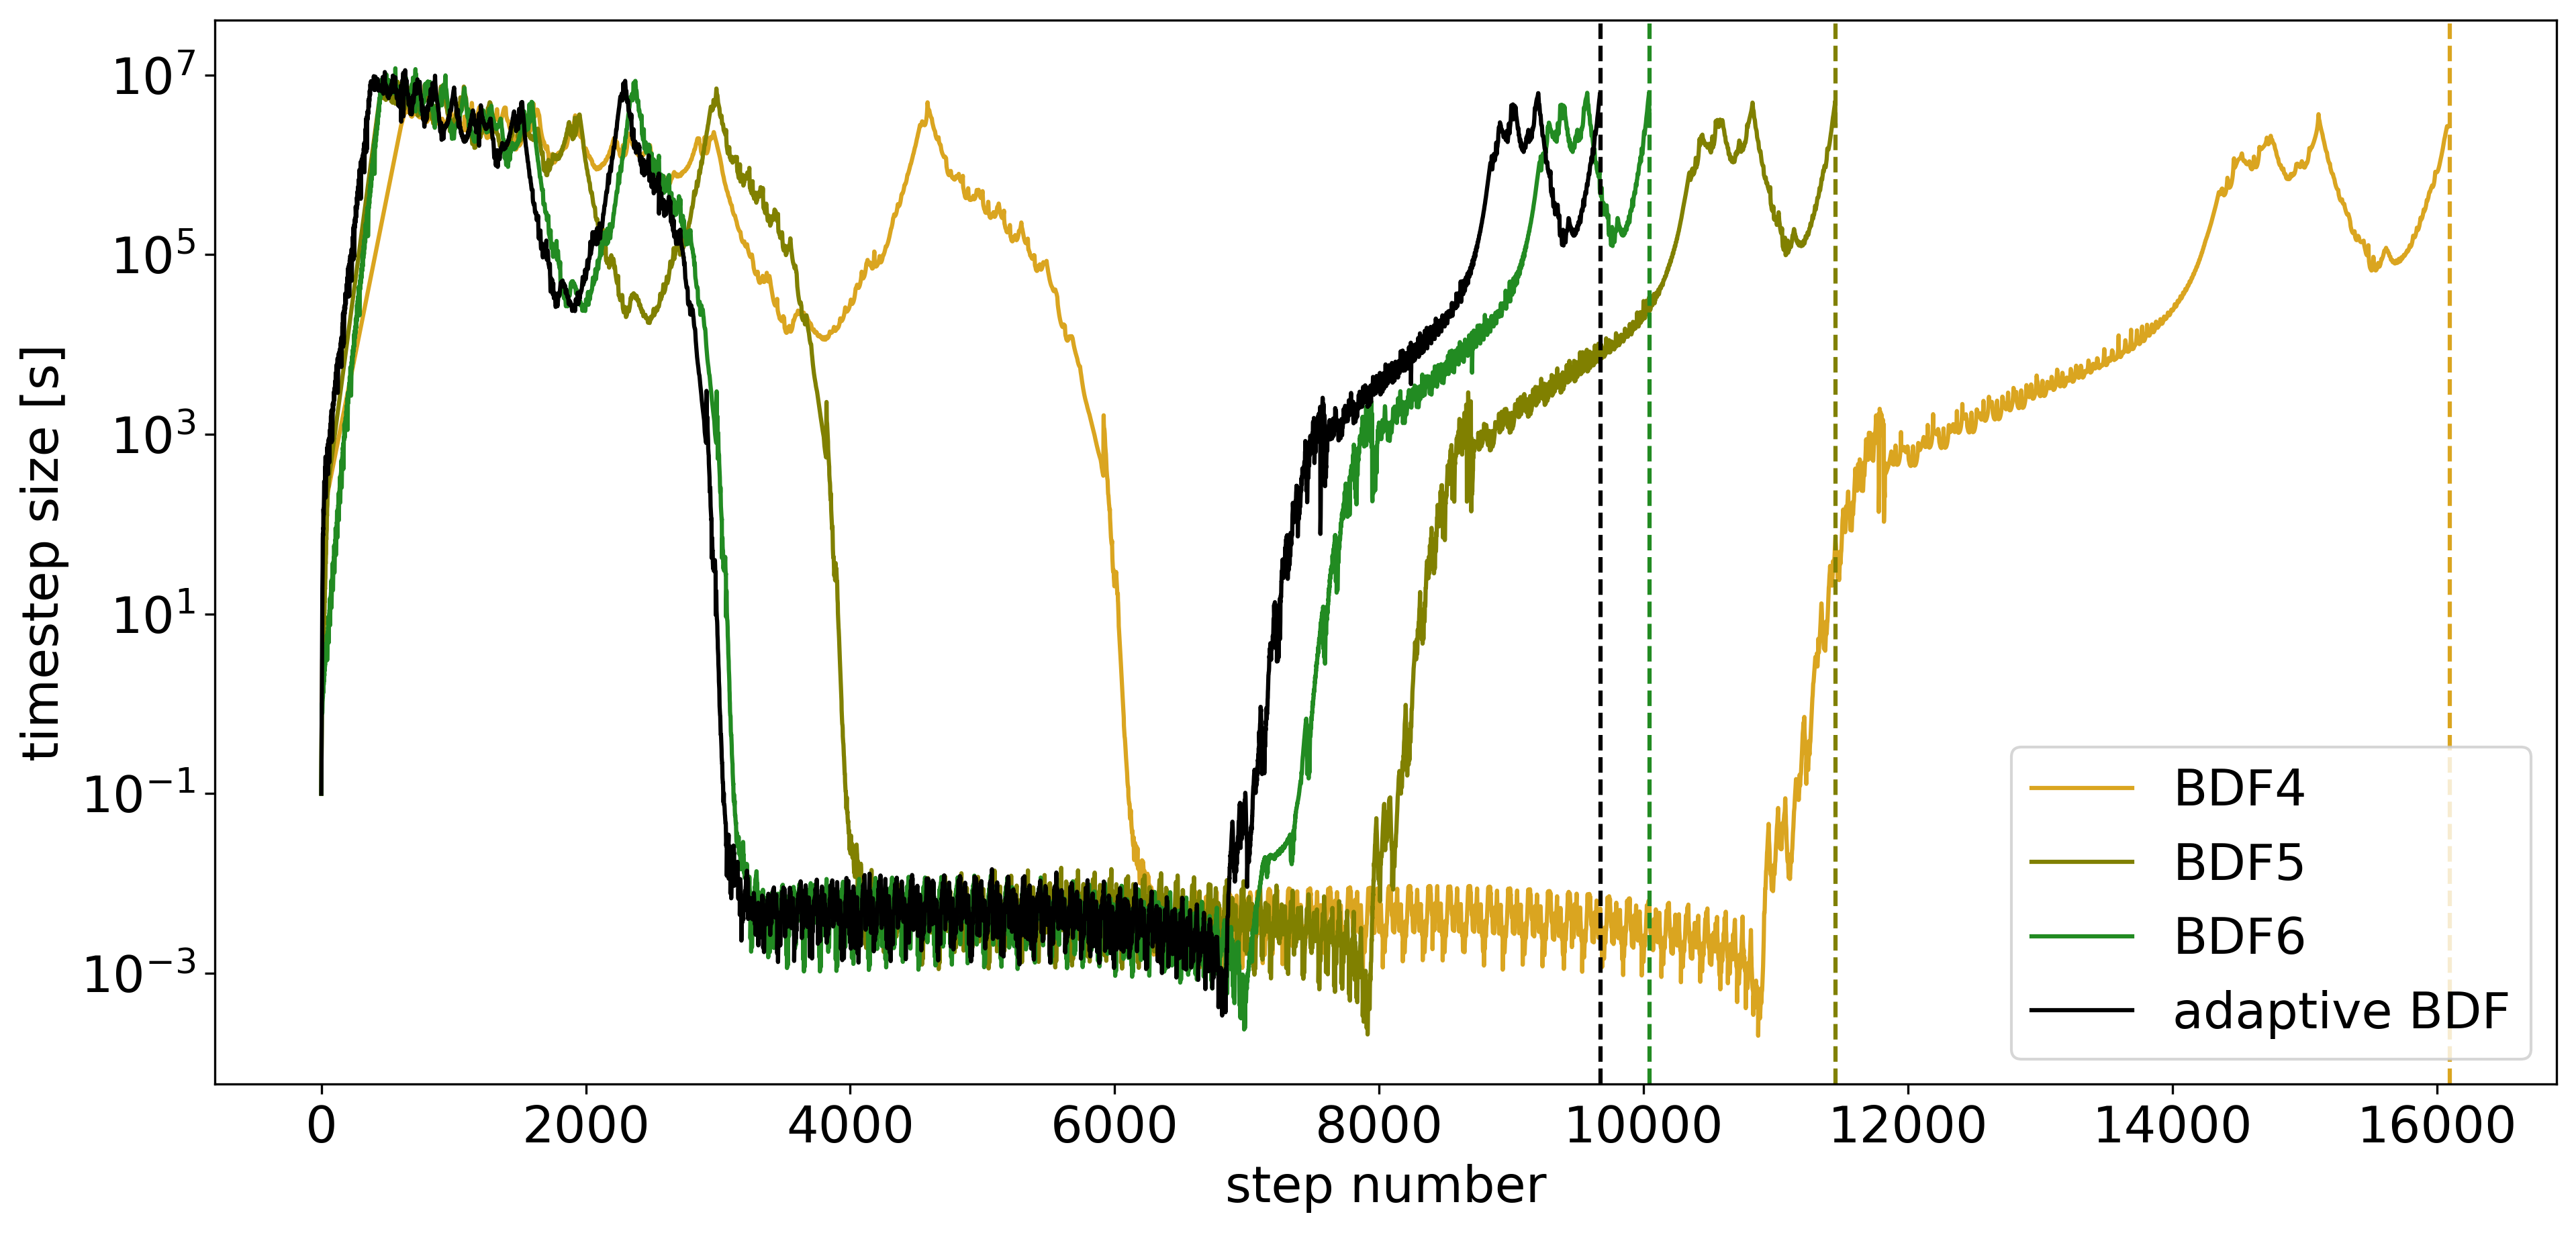
\includegraphics[width=0.8\textwidth]{images/TANDEMTimeAnalysisDifferentBDFOrders_Lagrange_ExtendedDAE_Size101_FULLTIME.png}
	\caption{Evolution of the time step size for the adaptive-order BDF method and for a selection of different fixed order methods on a domain with 101 fault elements using the extended DAE formulation.}
	\label{fig:BDFOrders_extended_DAE_compare_adaptiveBDF}
\end{figure}


\section{Scalability}
\label{sec:Results_Scalability}
The aim of this section is to investigate how the time integration scales with the problem size. To ensure comparability between the results, we set the tolerances such that the period between earthquakes and the slip increase are solved with similar accuracy, let us say to respectively $10^2$s and $10{-5}$m. From the analysis in \autoref{sec:Results_AccuracyTimeIntegration}, we can choose $t_a^S=10^{-8}$ and $t_a^S=10^{-5}$ for the aseismic and earthquake phases in first order formulations, and $t_r^V=10^{-8}$ and $t_r^V=10^{-7}$ in the second order ODE formulation. 

\begin{figure}[H]
	\centering
	\begin{subfigure}[b]{0.32\textwidth}
		\centering
		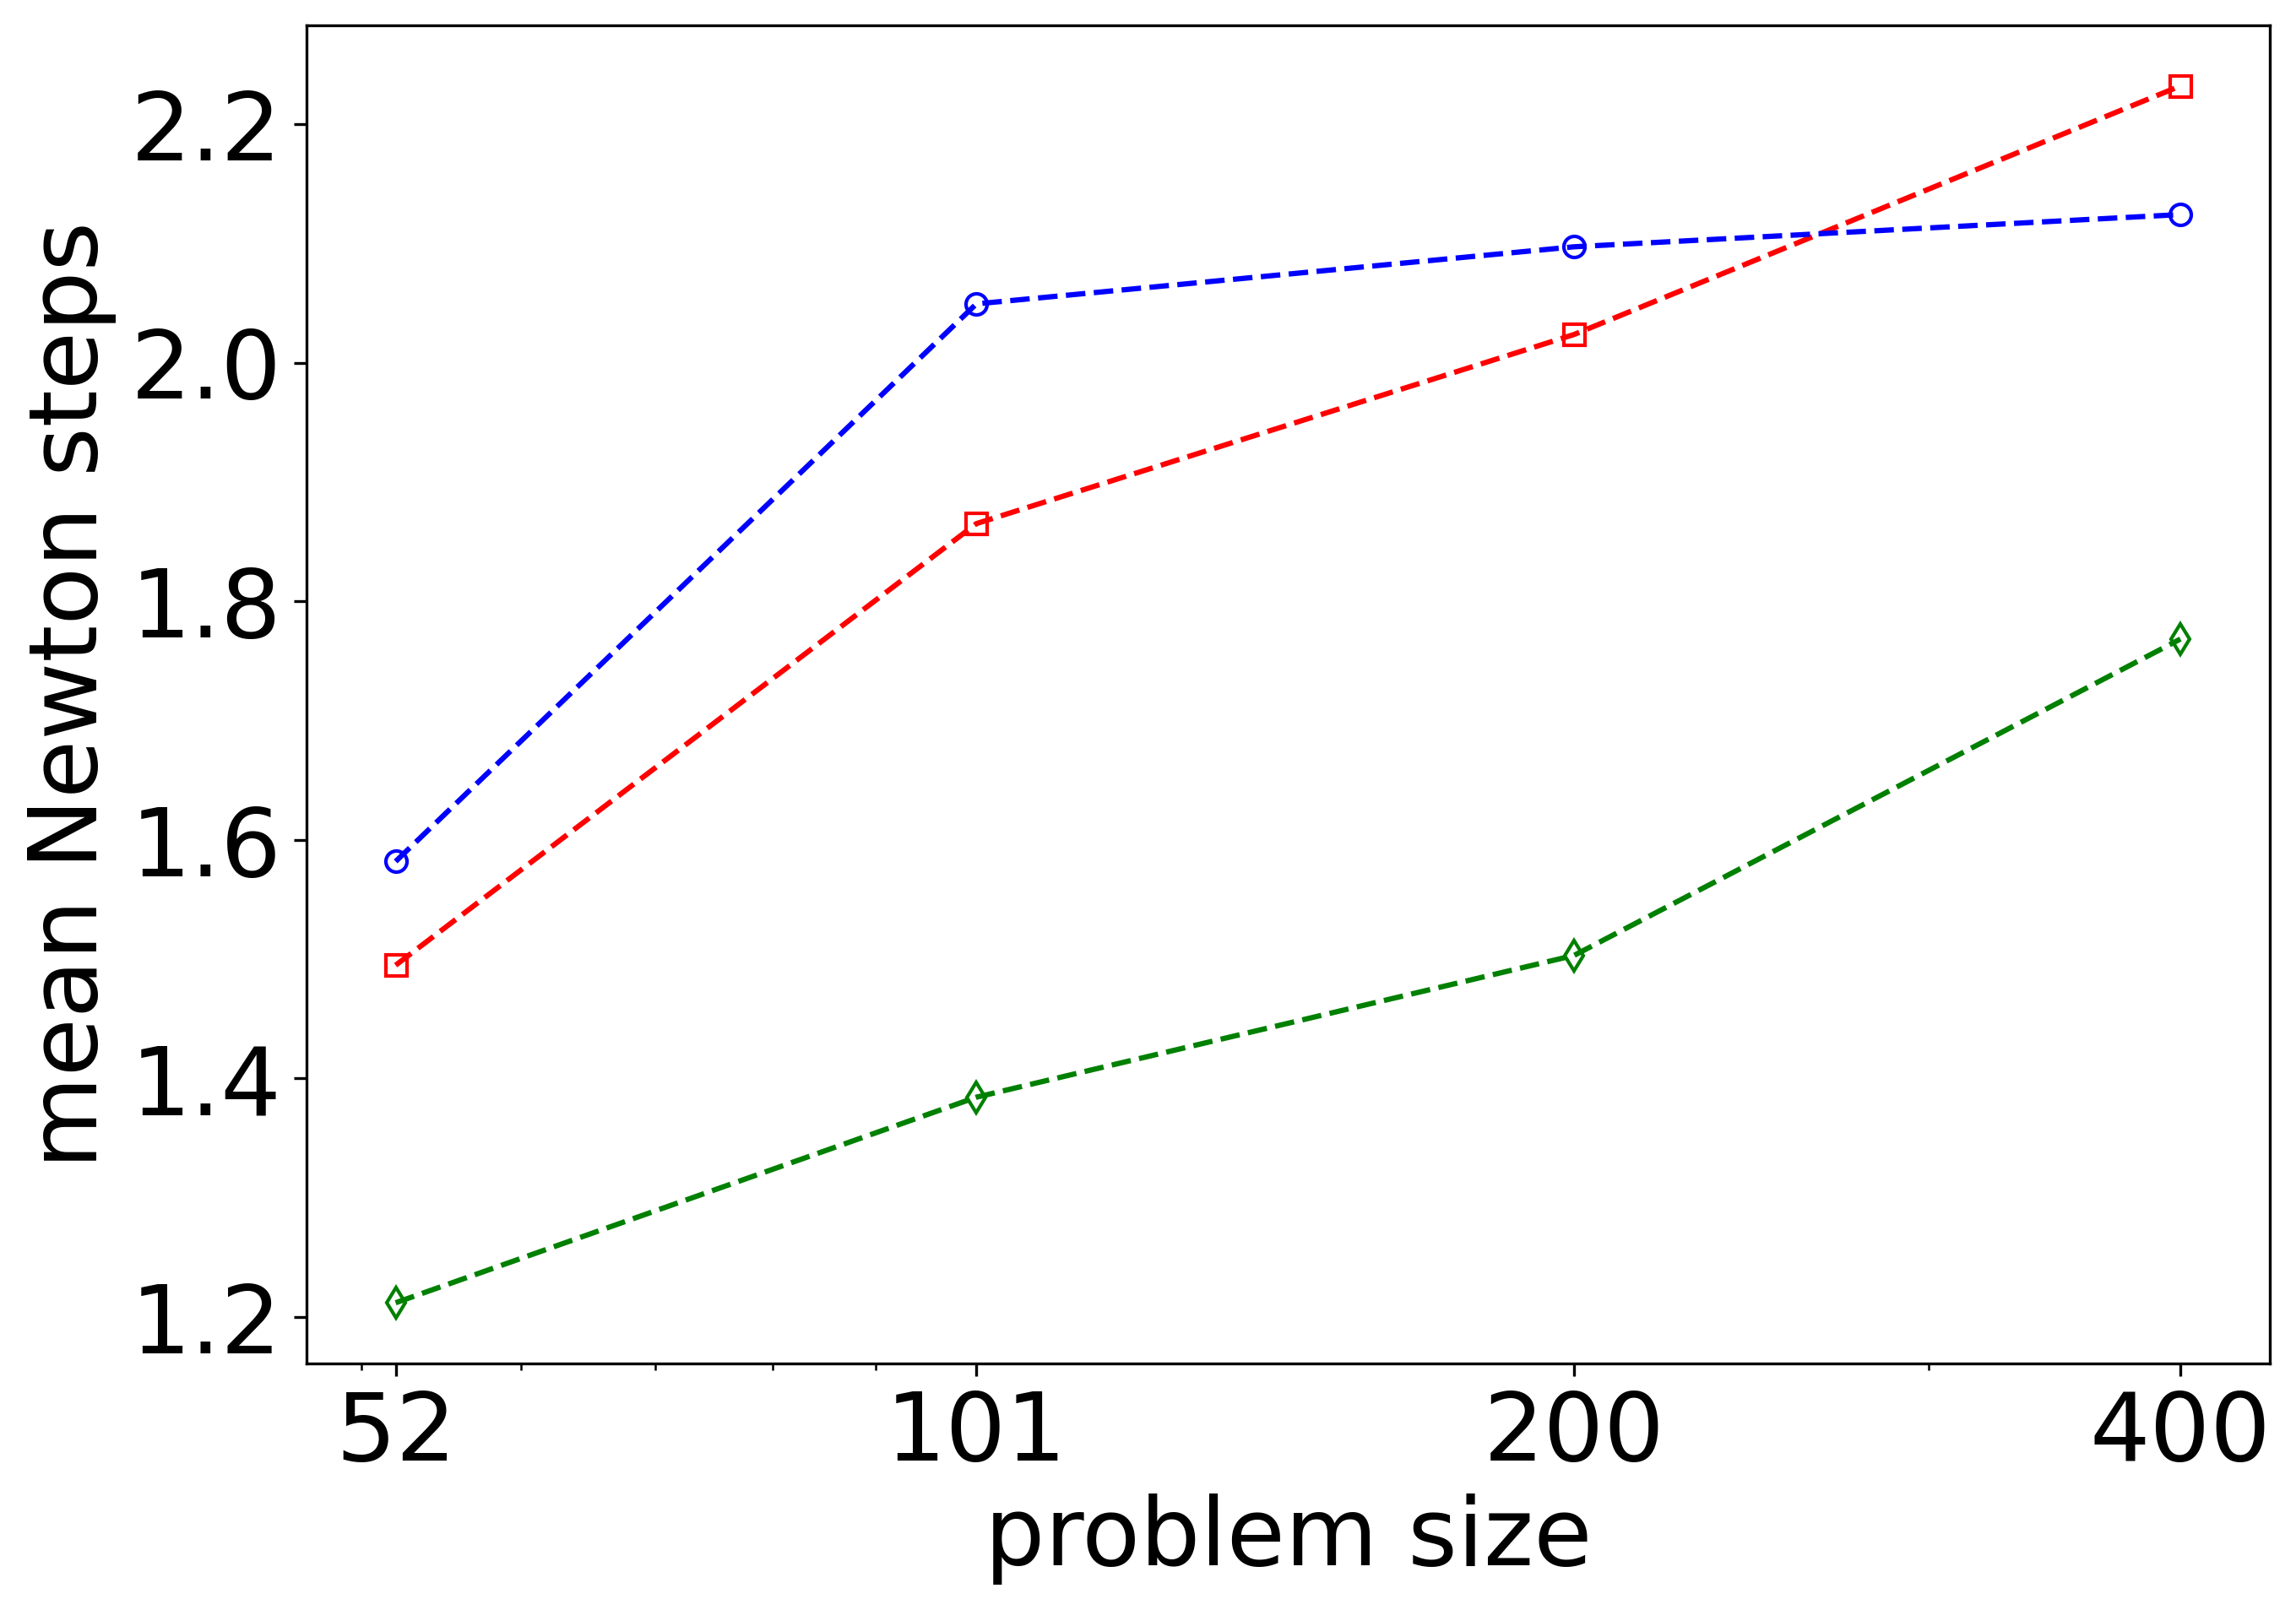
\includegraphics[width=1\textwidth]{images/TANDEM_averageNumberNewtonSteps.png}
		\subcaption{Average number of Newton steps per timestep \\ \ } 
	\end{subfigure} 
	\begin{subfigure}[b]{0.32\textwidth}
		\centering
		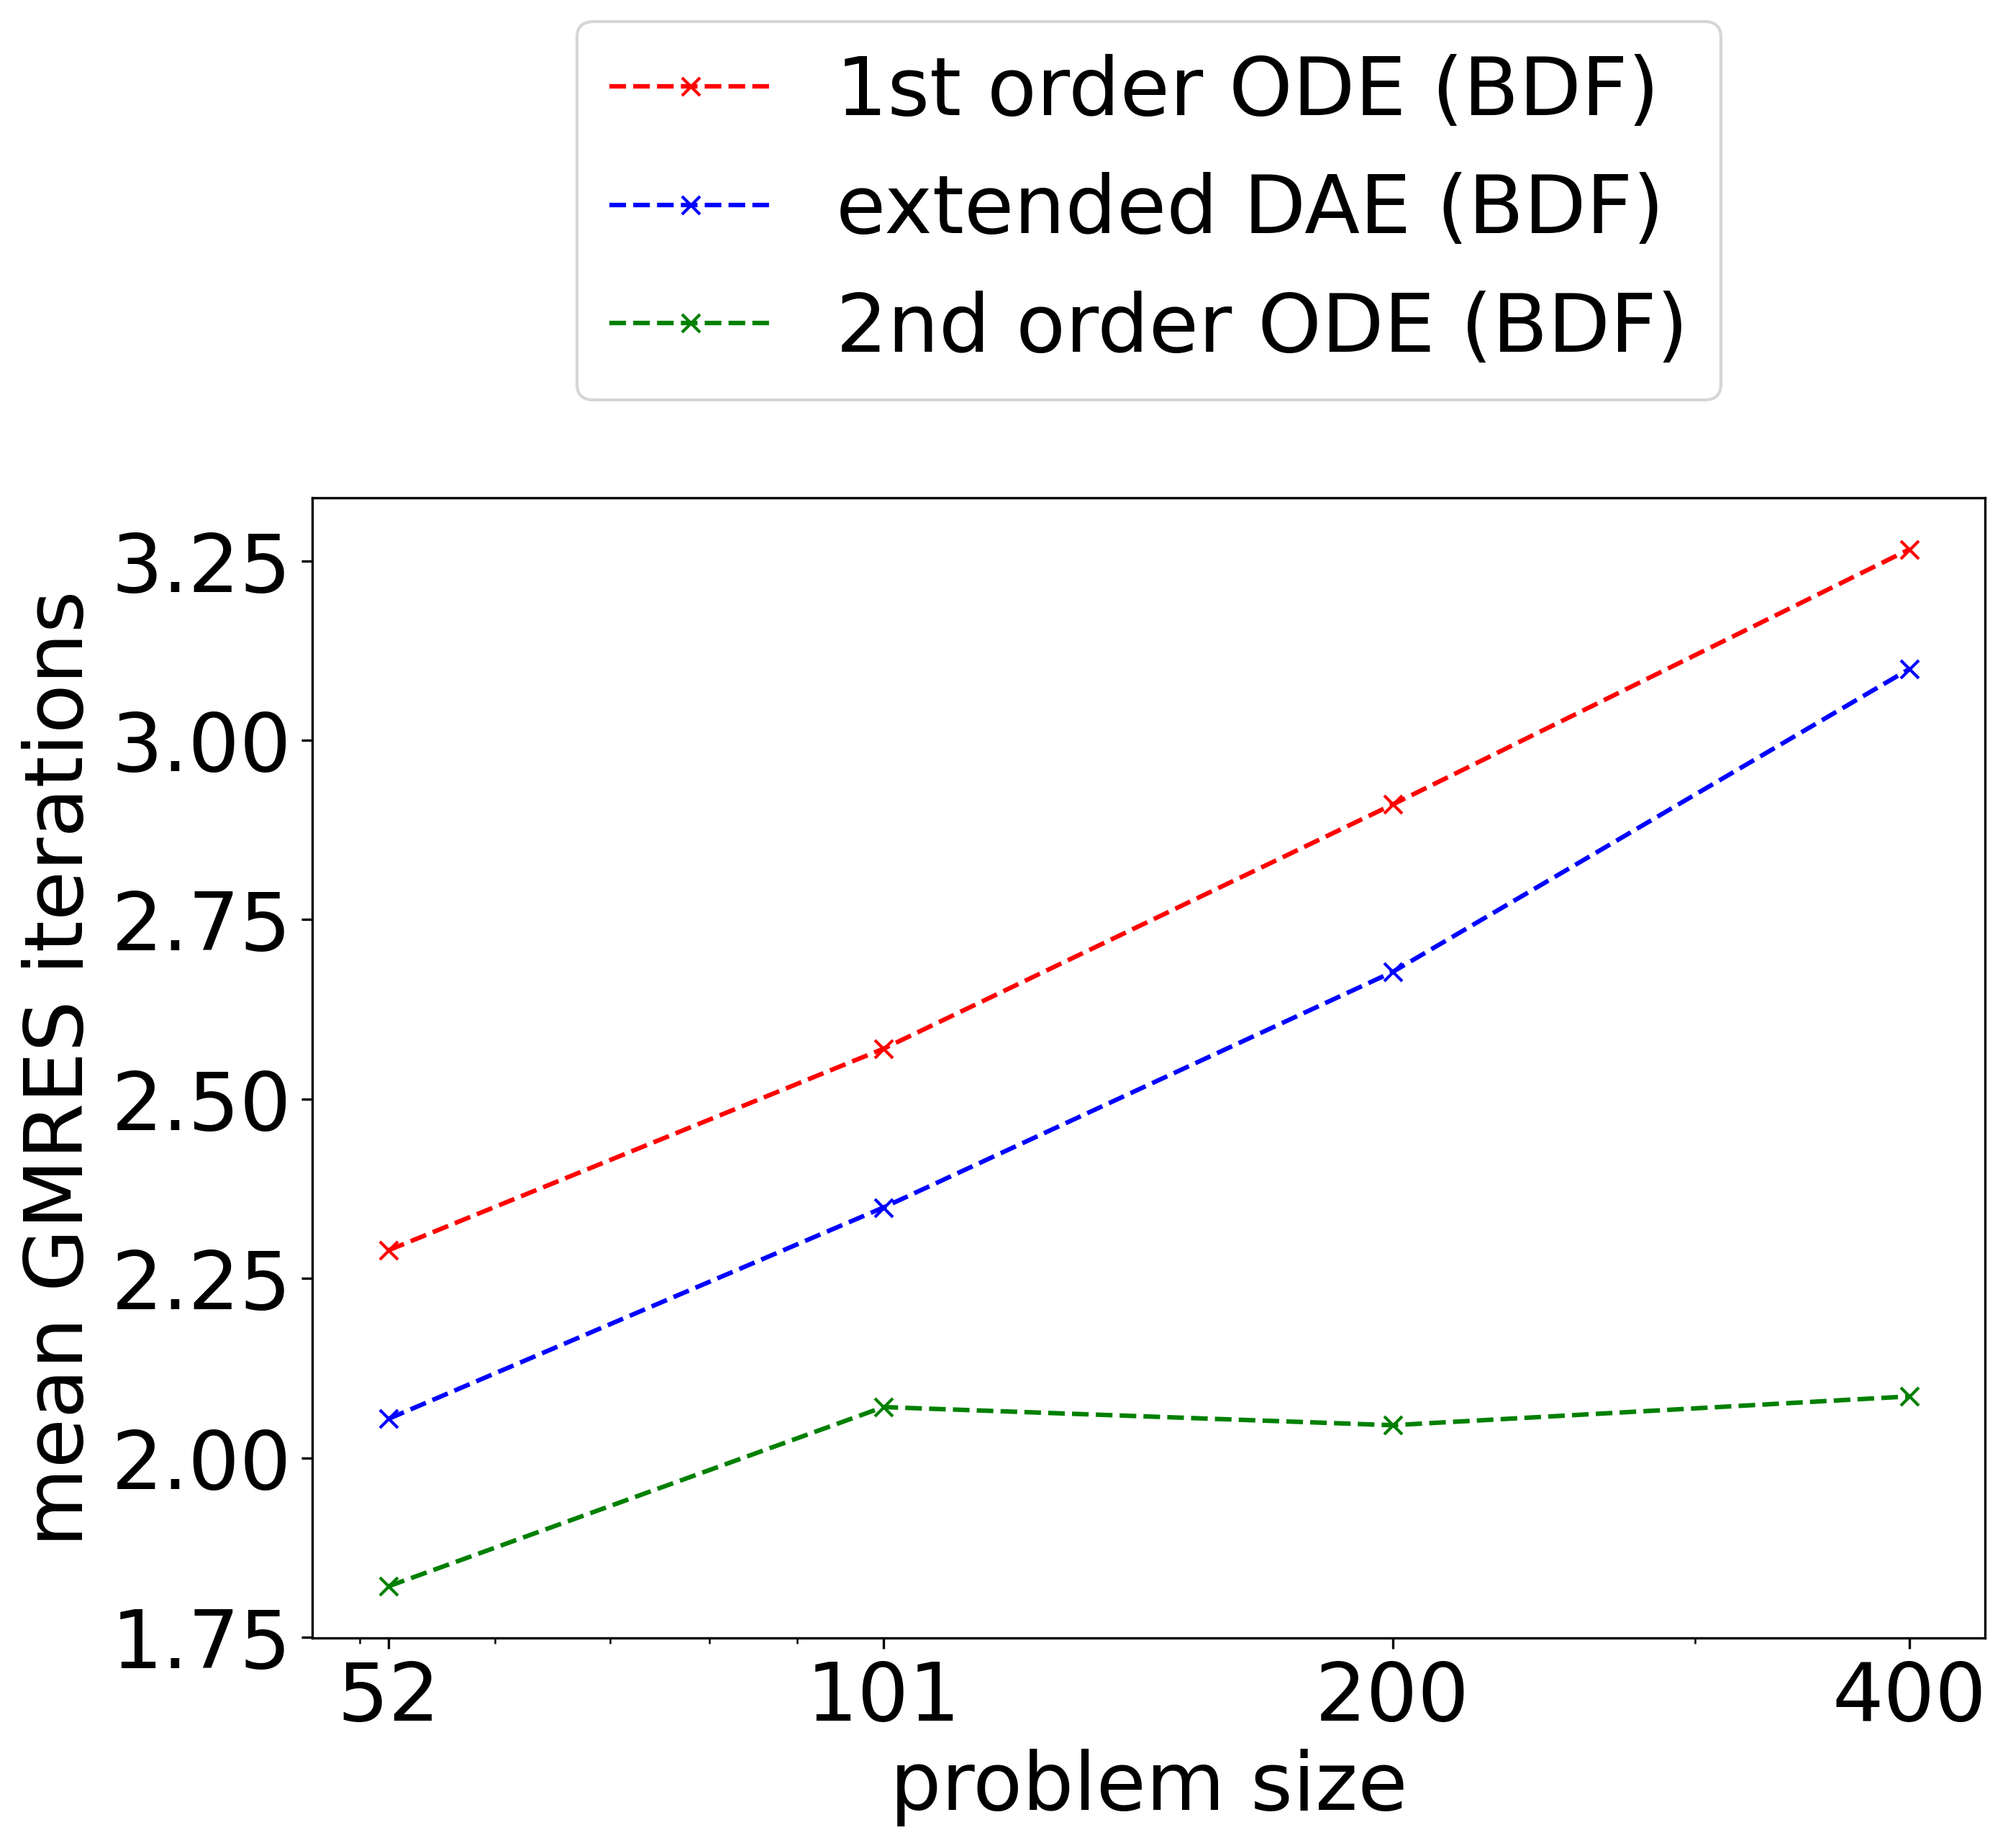
\includegraphics[width=1.03\textwidth]{images/TANDEM_averageNumberKSPIteration.png}
		\subcaption{Average iteration number of the linear solver per Newton step} 
	\end{subfigure}
	\begin{subfigure}[b]{0.32\textwidth}
		\centering
		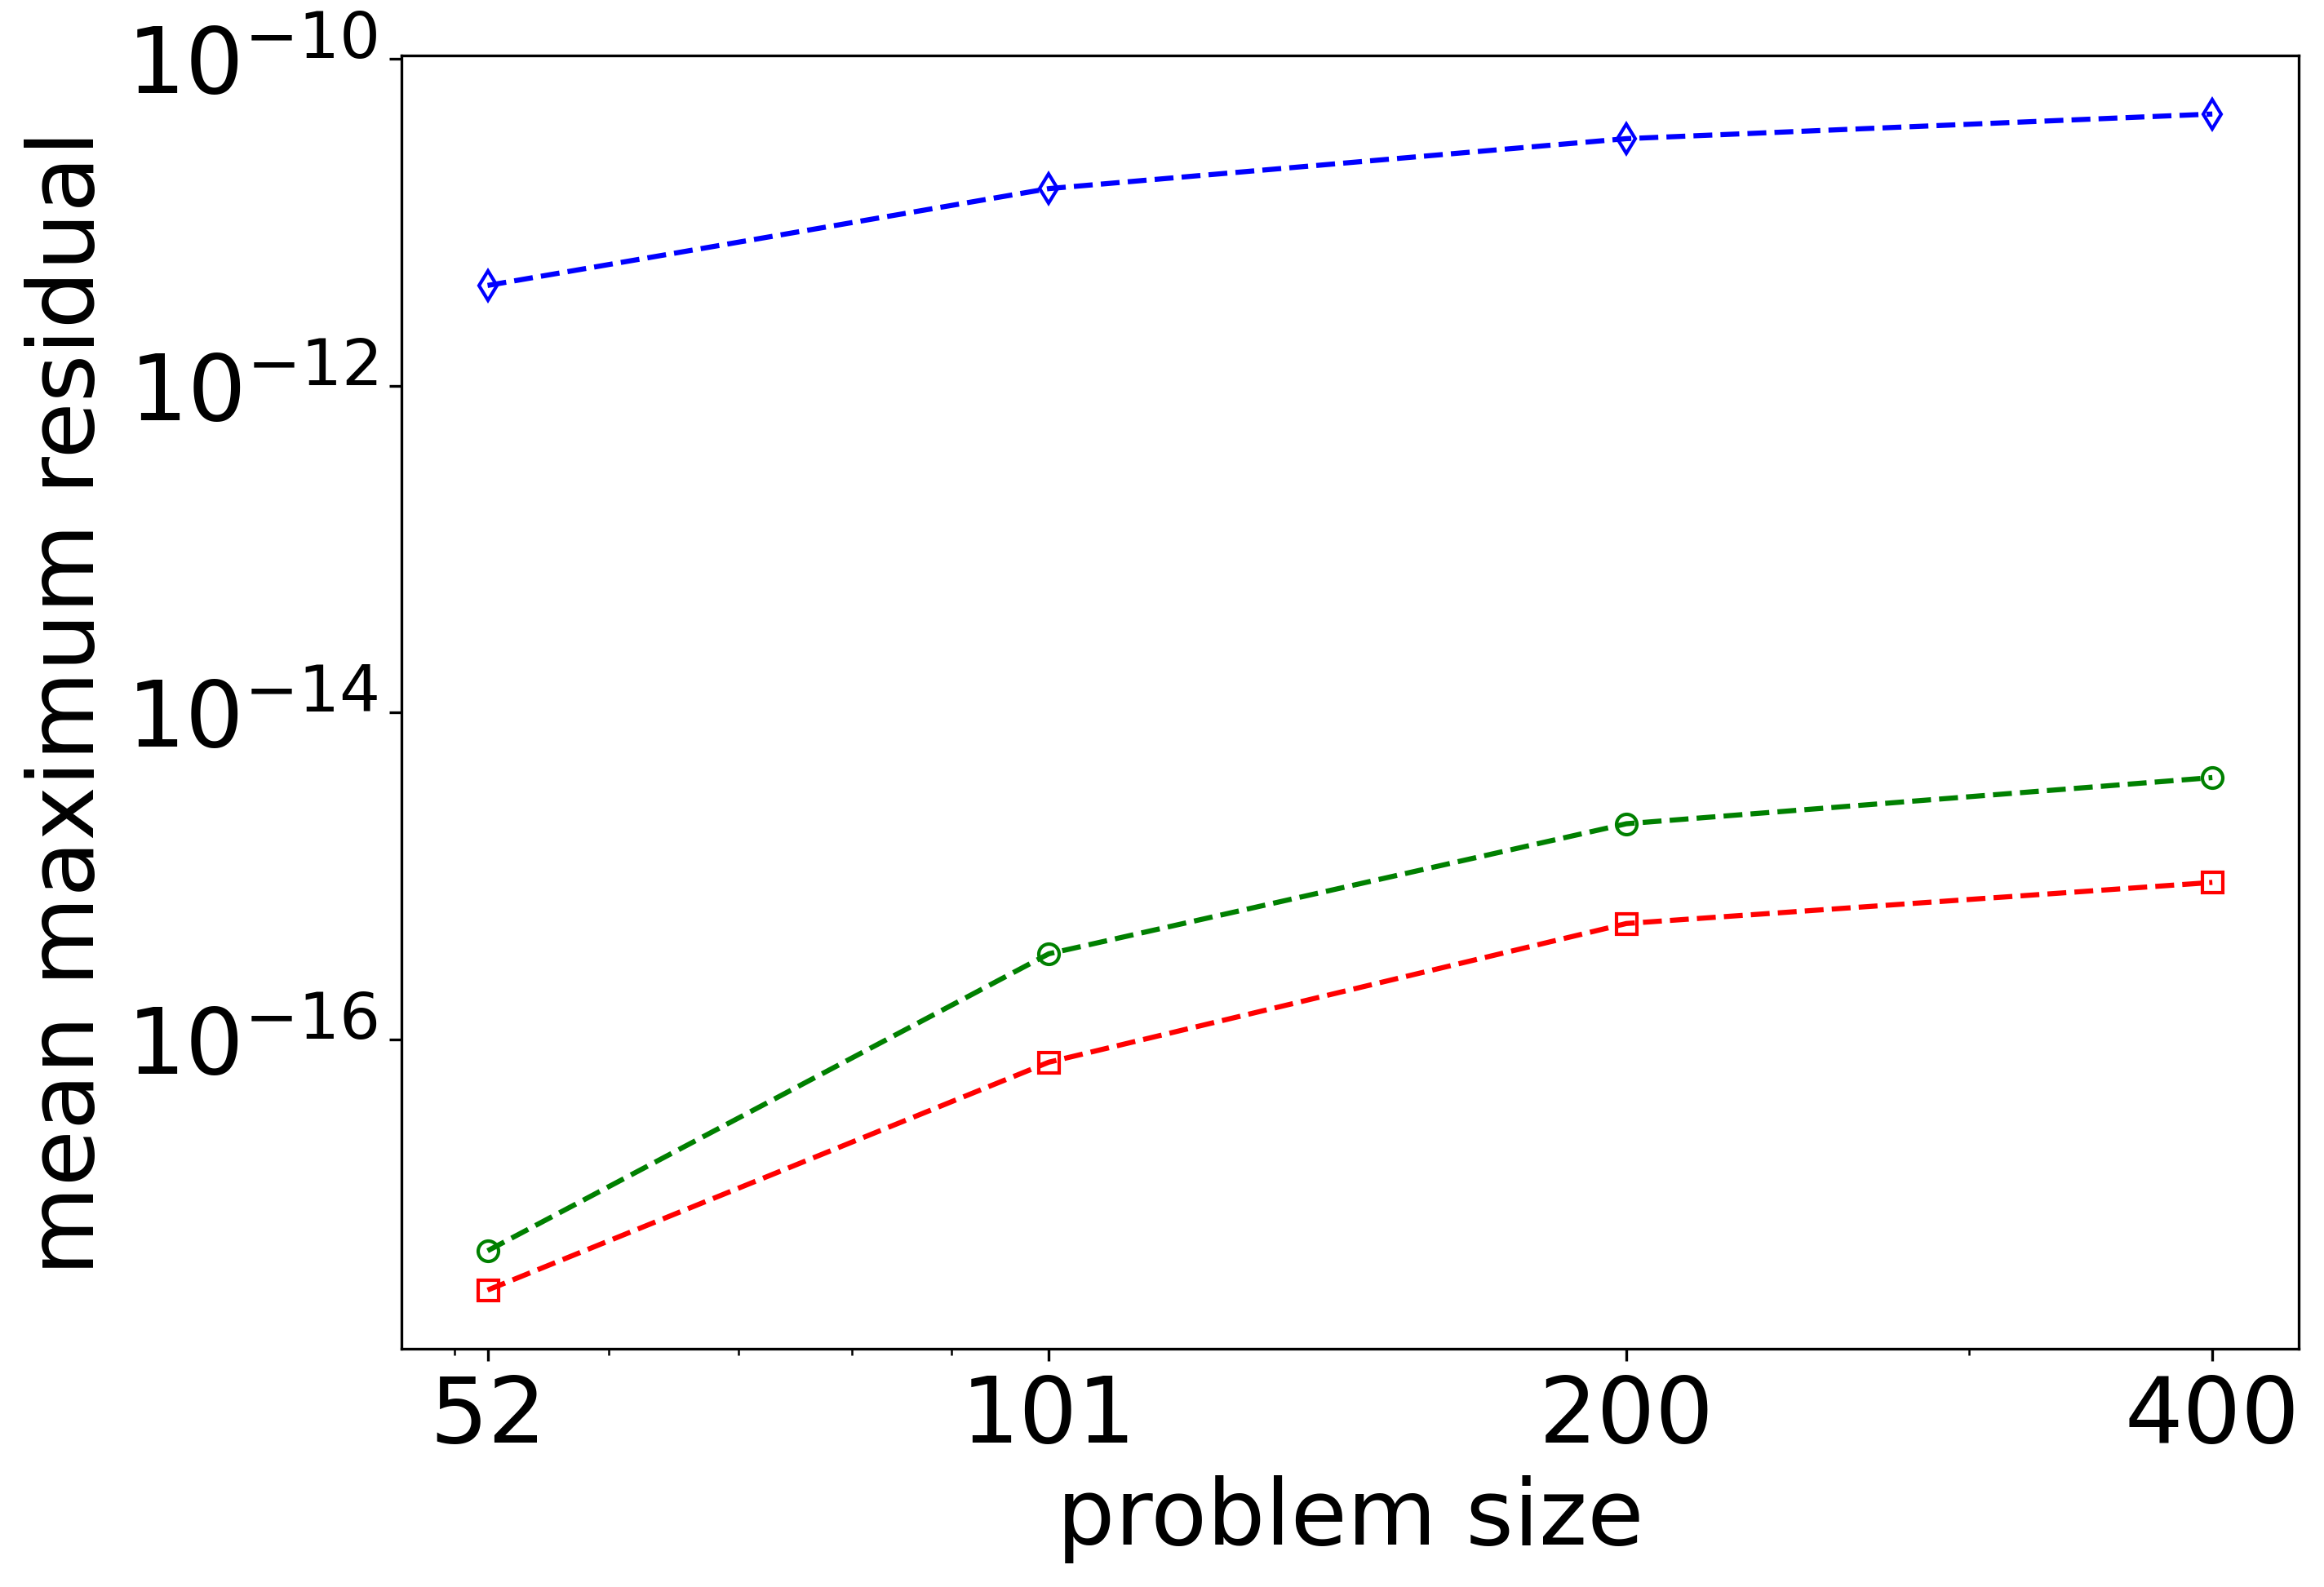
\includegraphics[width=1\textwidth]{images/TANDEM_maximumResidualNorm.png}
		\subcaption{Geometric mean of the final maximum norm of the residual} 
	\end{subfigure}
	\caption{Indicators of the Newton iteration for the implicit formulations with different problem sizes. Note that each timestep includes one RHS evaluation before the Newton iteration}
	\label{fig:implicit_methods_scalabilty_iterations}
\end{figure}

\begin{figure}[H]
	\centering
	\begin{subfigure}[b]{0.32\textwidth}
		\centering
		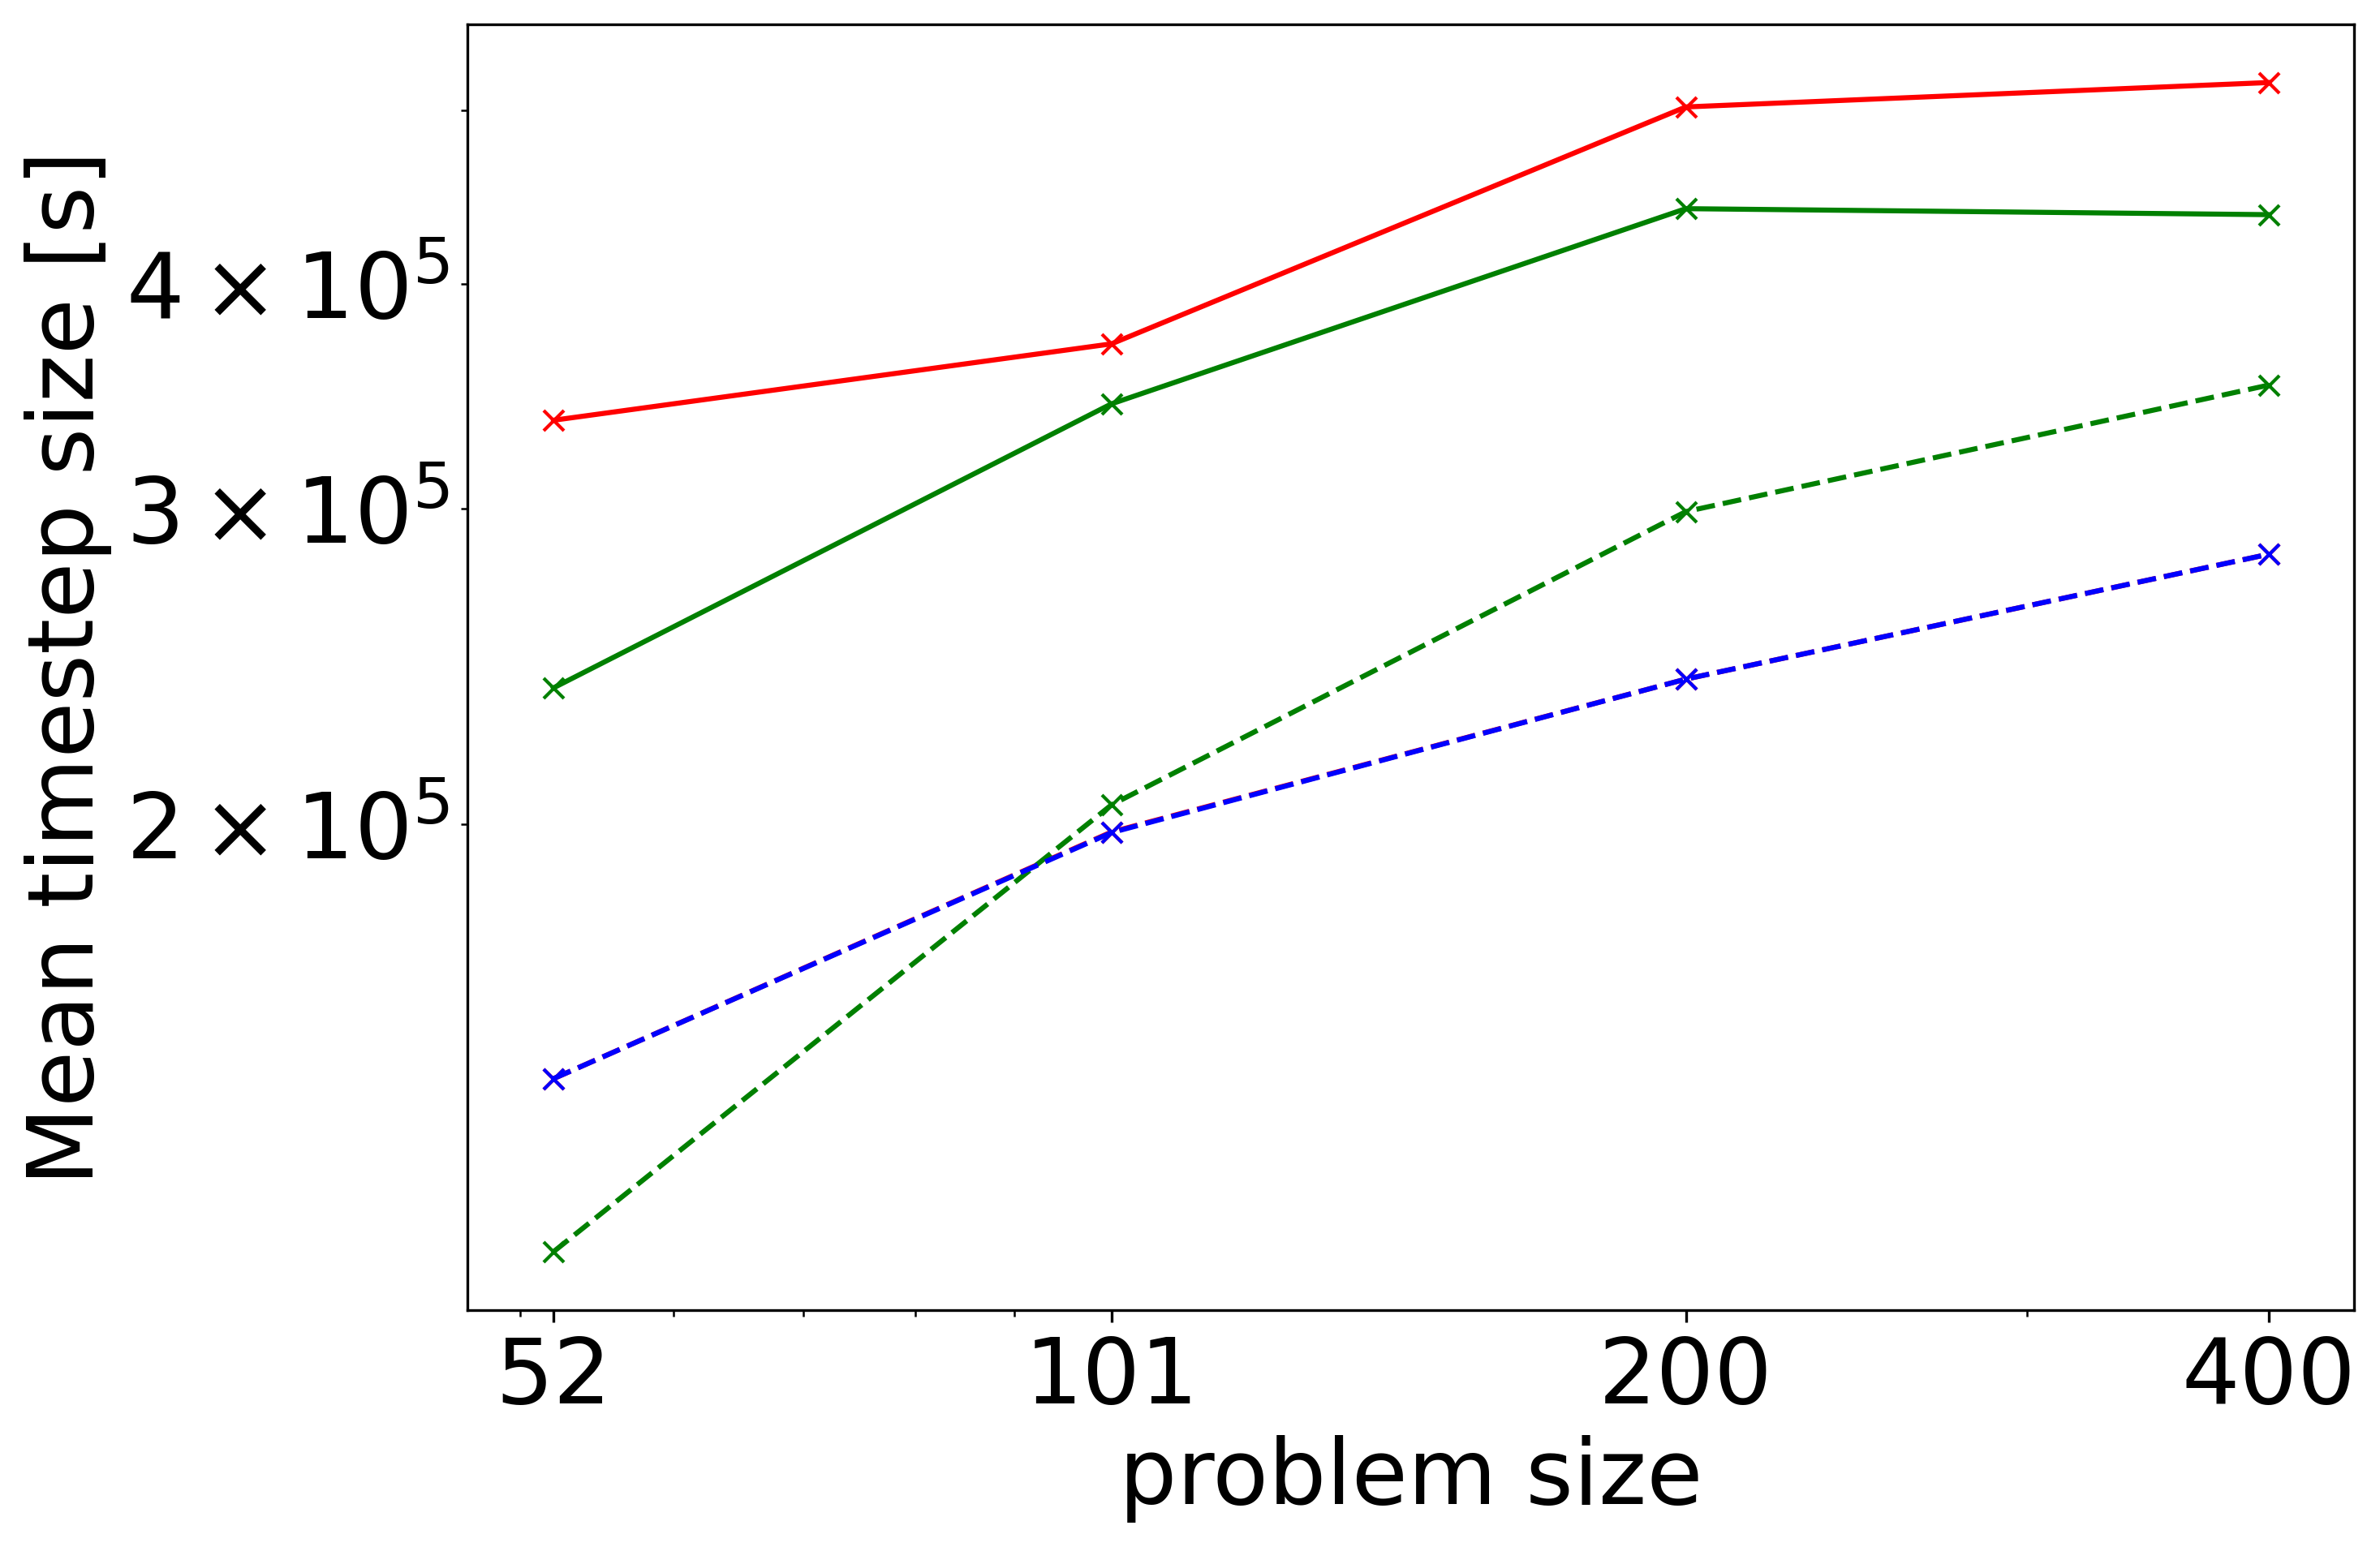
\includegraphics[width=1\textwidth]{images/TANDEM_MeanTimeStepSize_AseismicPhase.png}
		\subcaption{Geometric mean of the timestep size in the aseismic phase}
	\end{subfigure}
	\begin{subfigure}[b]{0.32\textwidth}
		\centering \hspace{-0.75cm}
		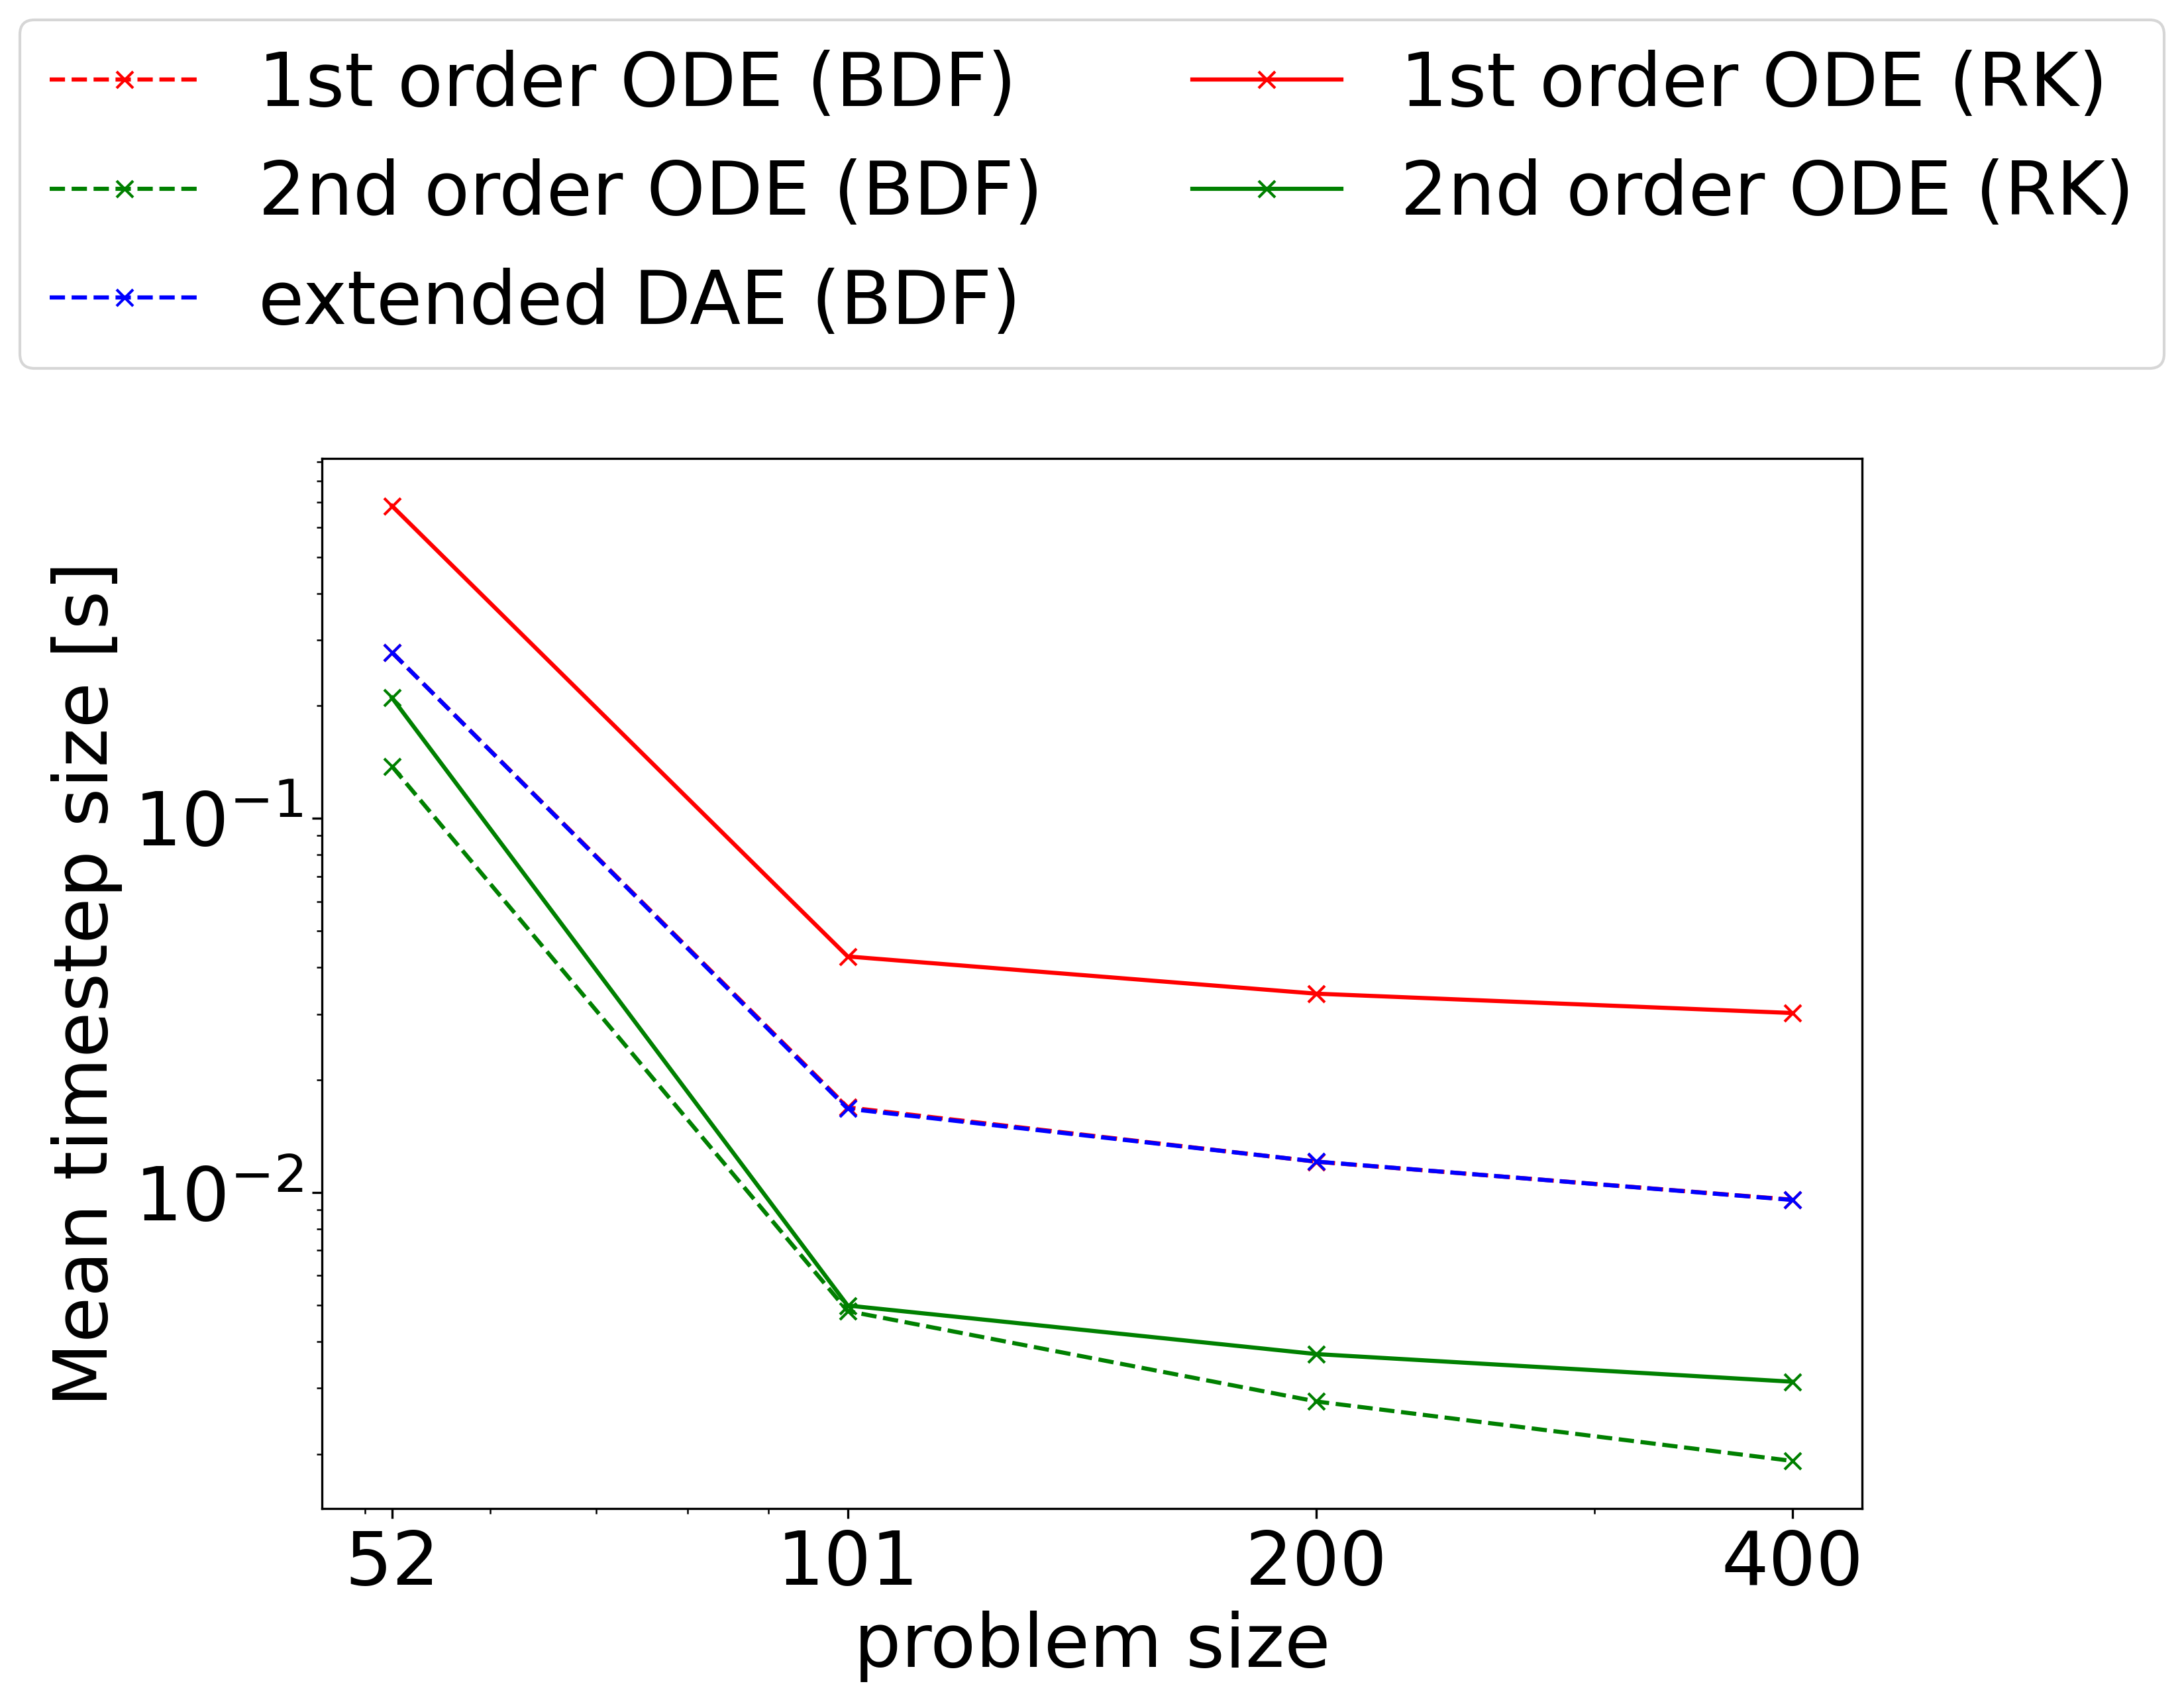
\includegraphics[width=1.14\textwidth]{images/TANDEM_MeanTimeStepSize_EarthquakePhase.png}
		\subcaption{Geometric mean of the timestep size in the earthquake phase} 
	\end{subfigure}
	\begin{subfigure}[b]{0.32\textwidth}
		\centering
		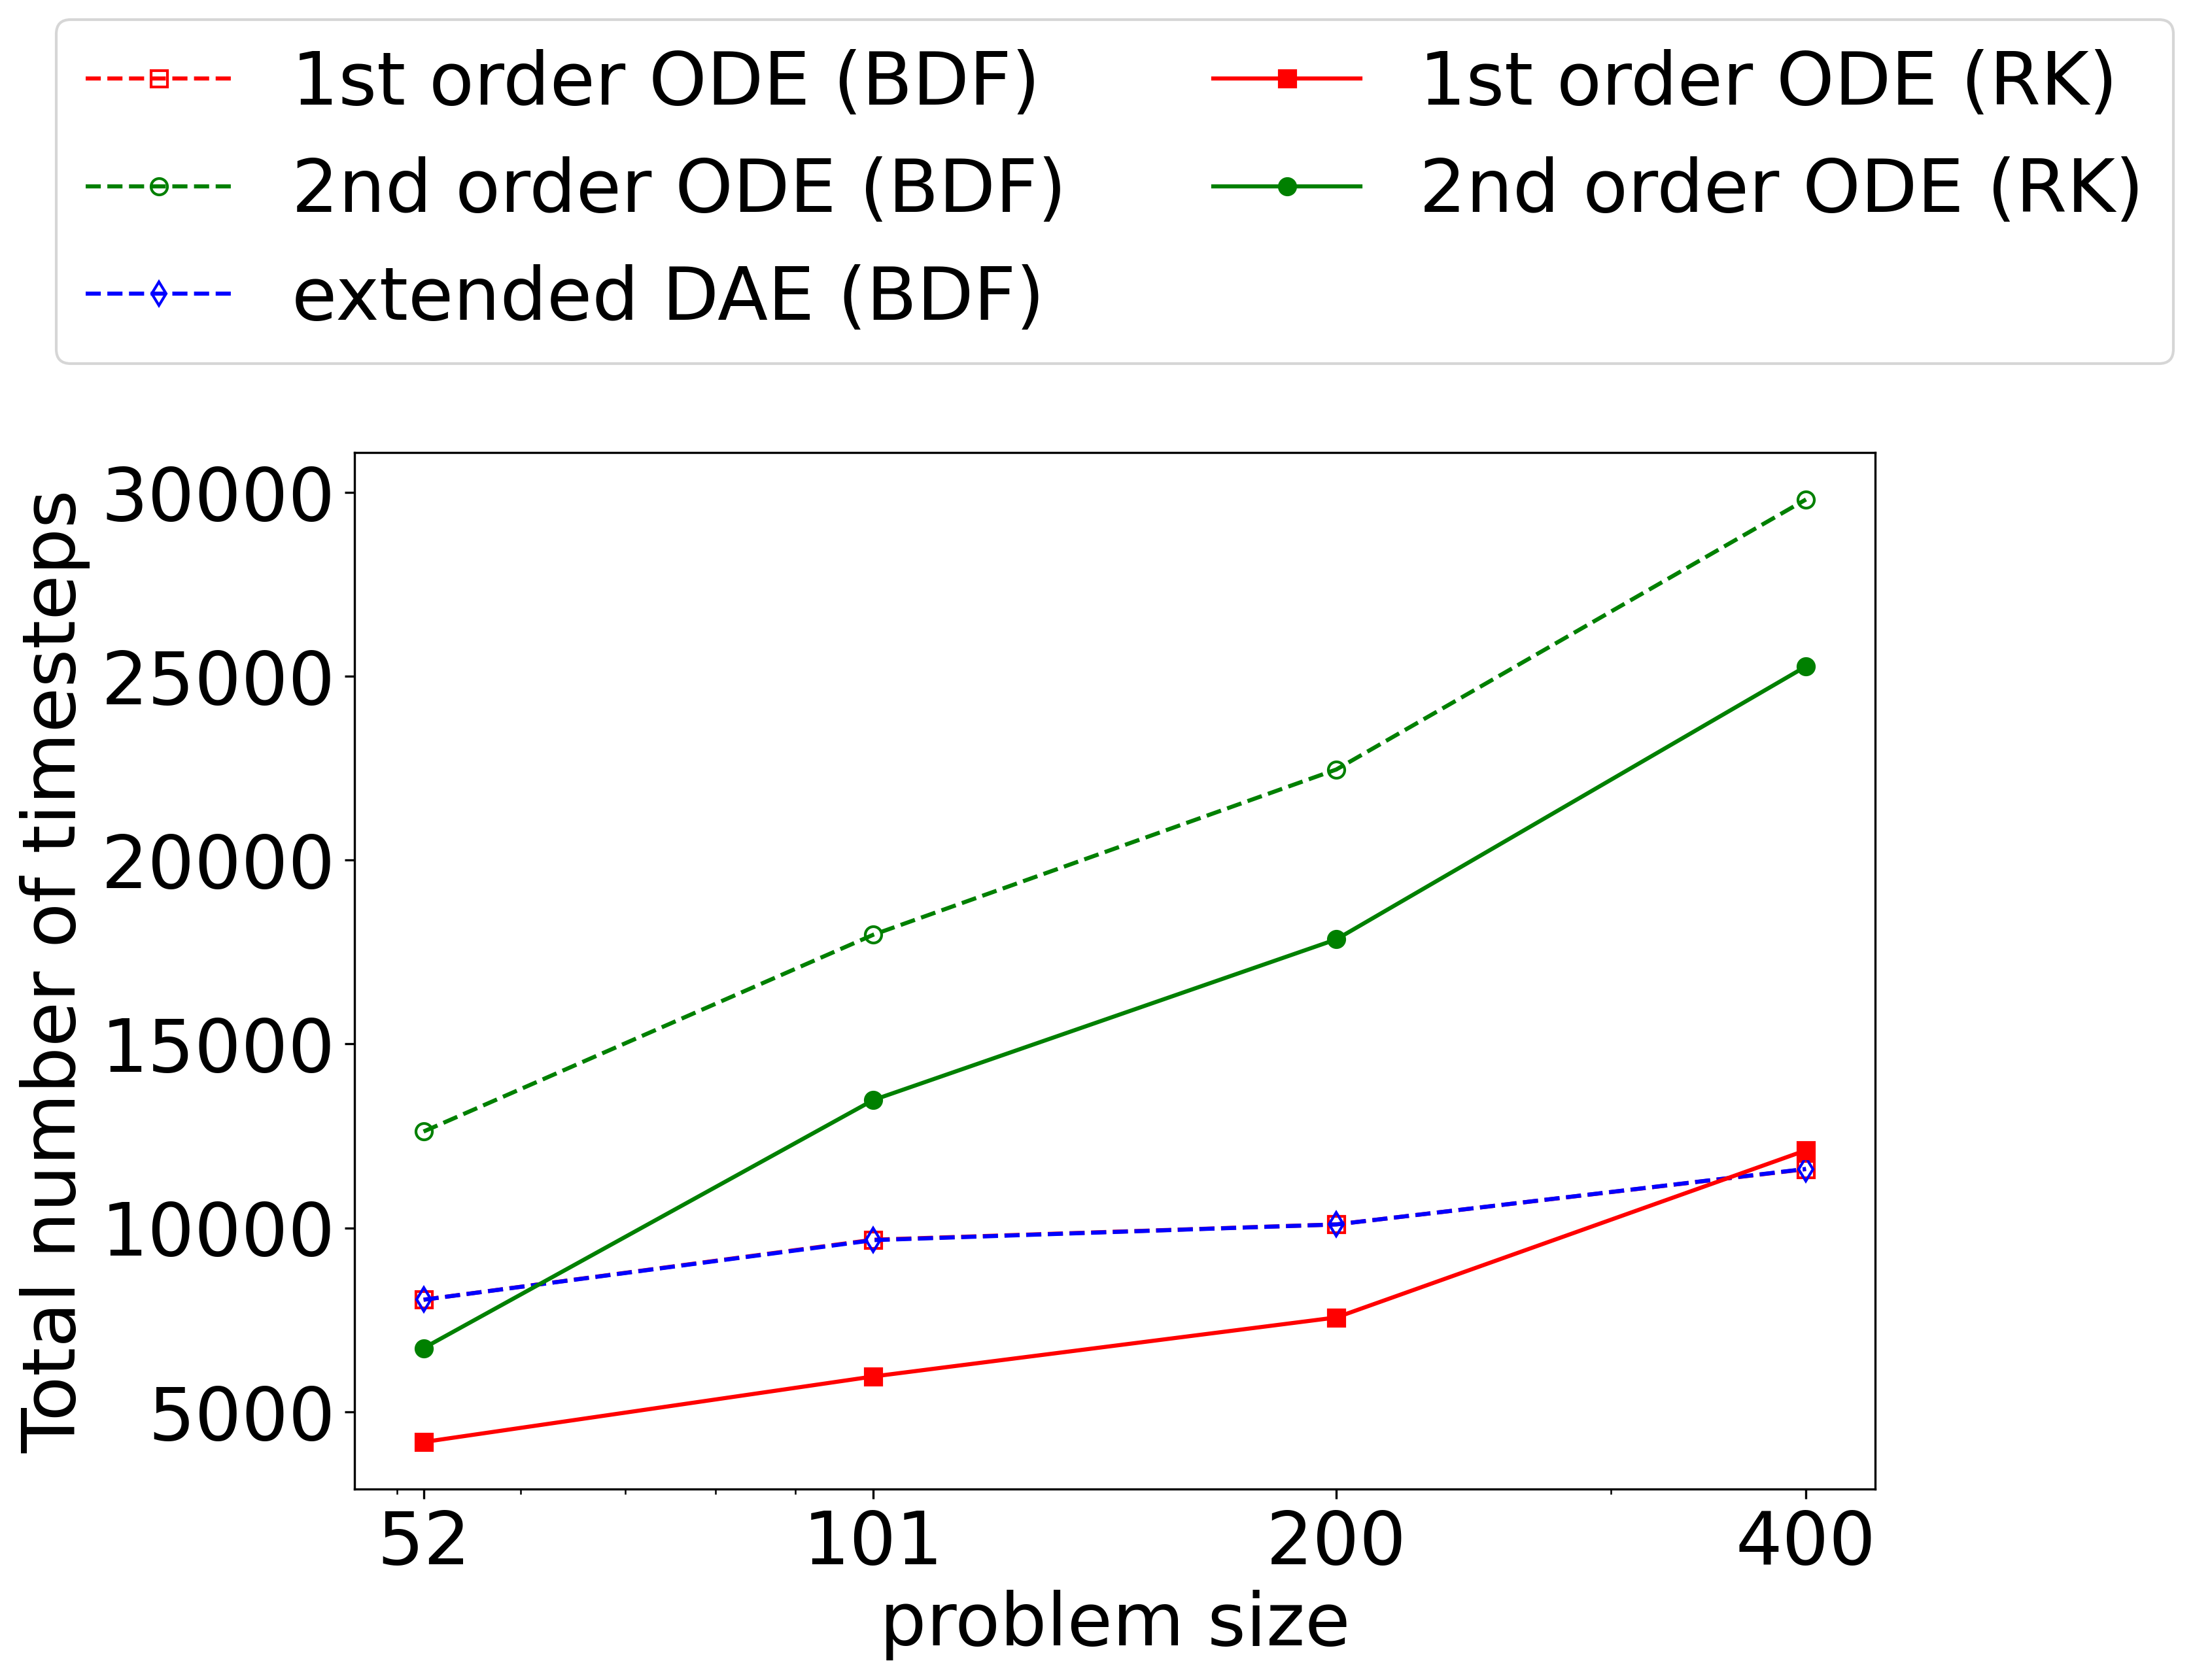
\includegraphics[width=1\textwidth]{images/TANDEM_NumberTimeSteps_differentSizes.png}
		\subcaption{Total number of timesteps \\ \ \\ \ }
	\end{subfigure}
	\caption{Behaviour of the timestep with different problem sizes.}
	\label{fig:scalabilty_timeStepSizes}
\end{figure}

\begin{figure}[H]
	\centering
	\begin{subfigure}[b]{0.32\textwidth}
		\centering
		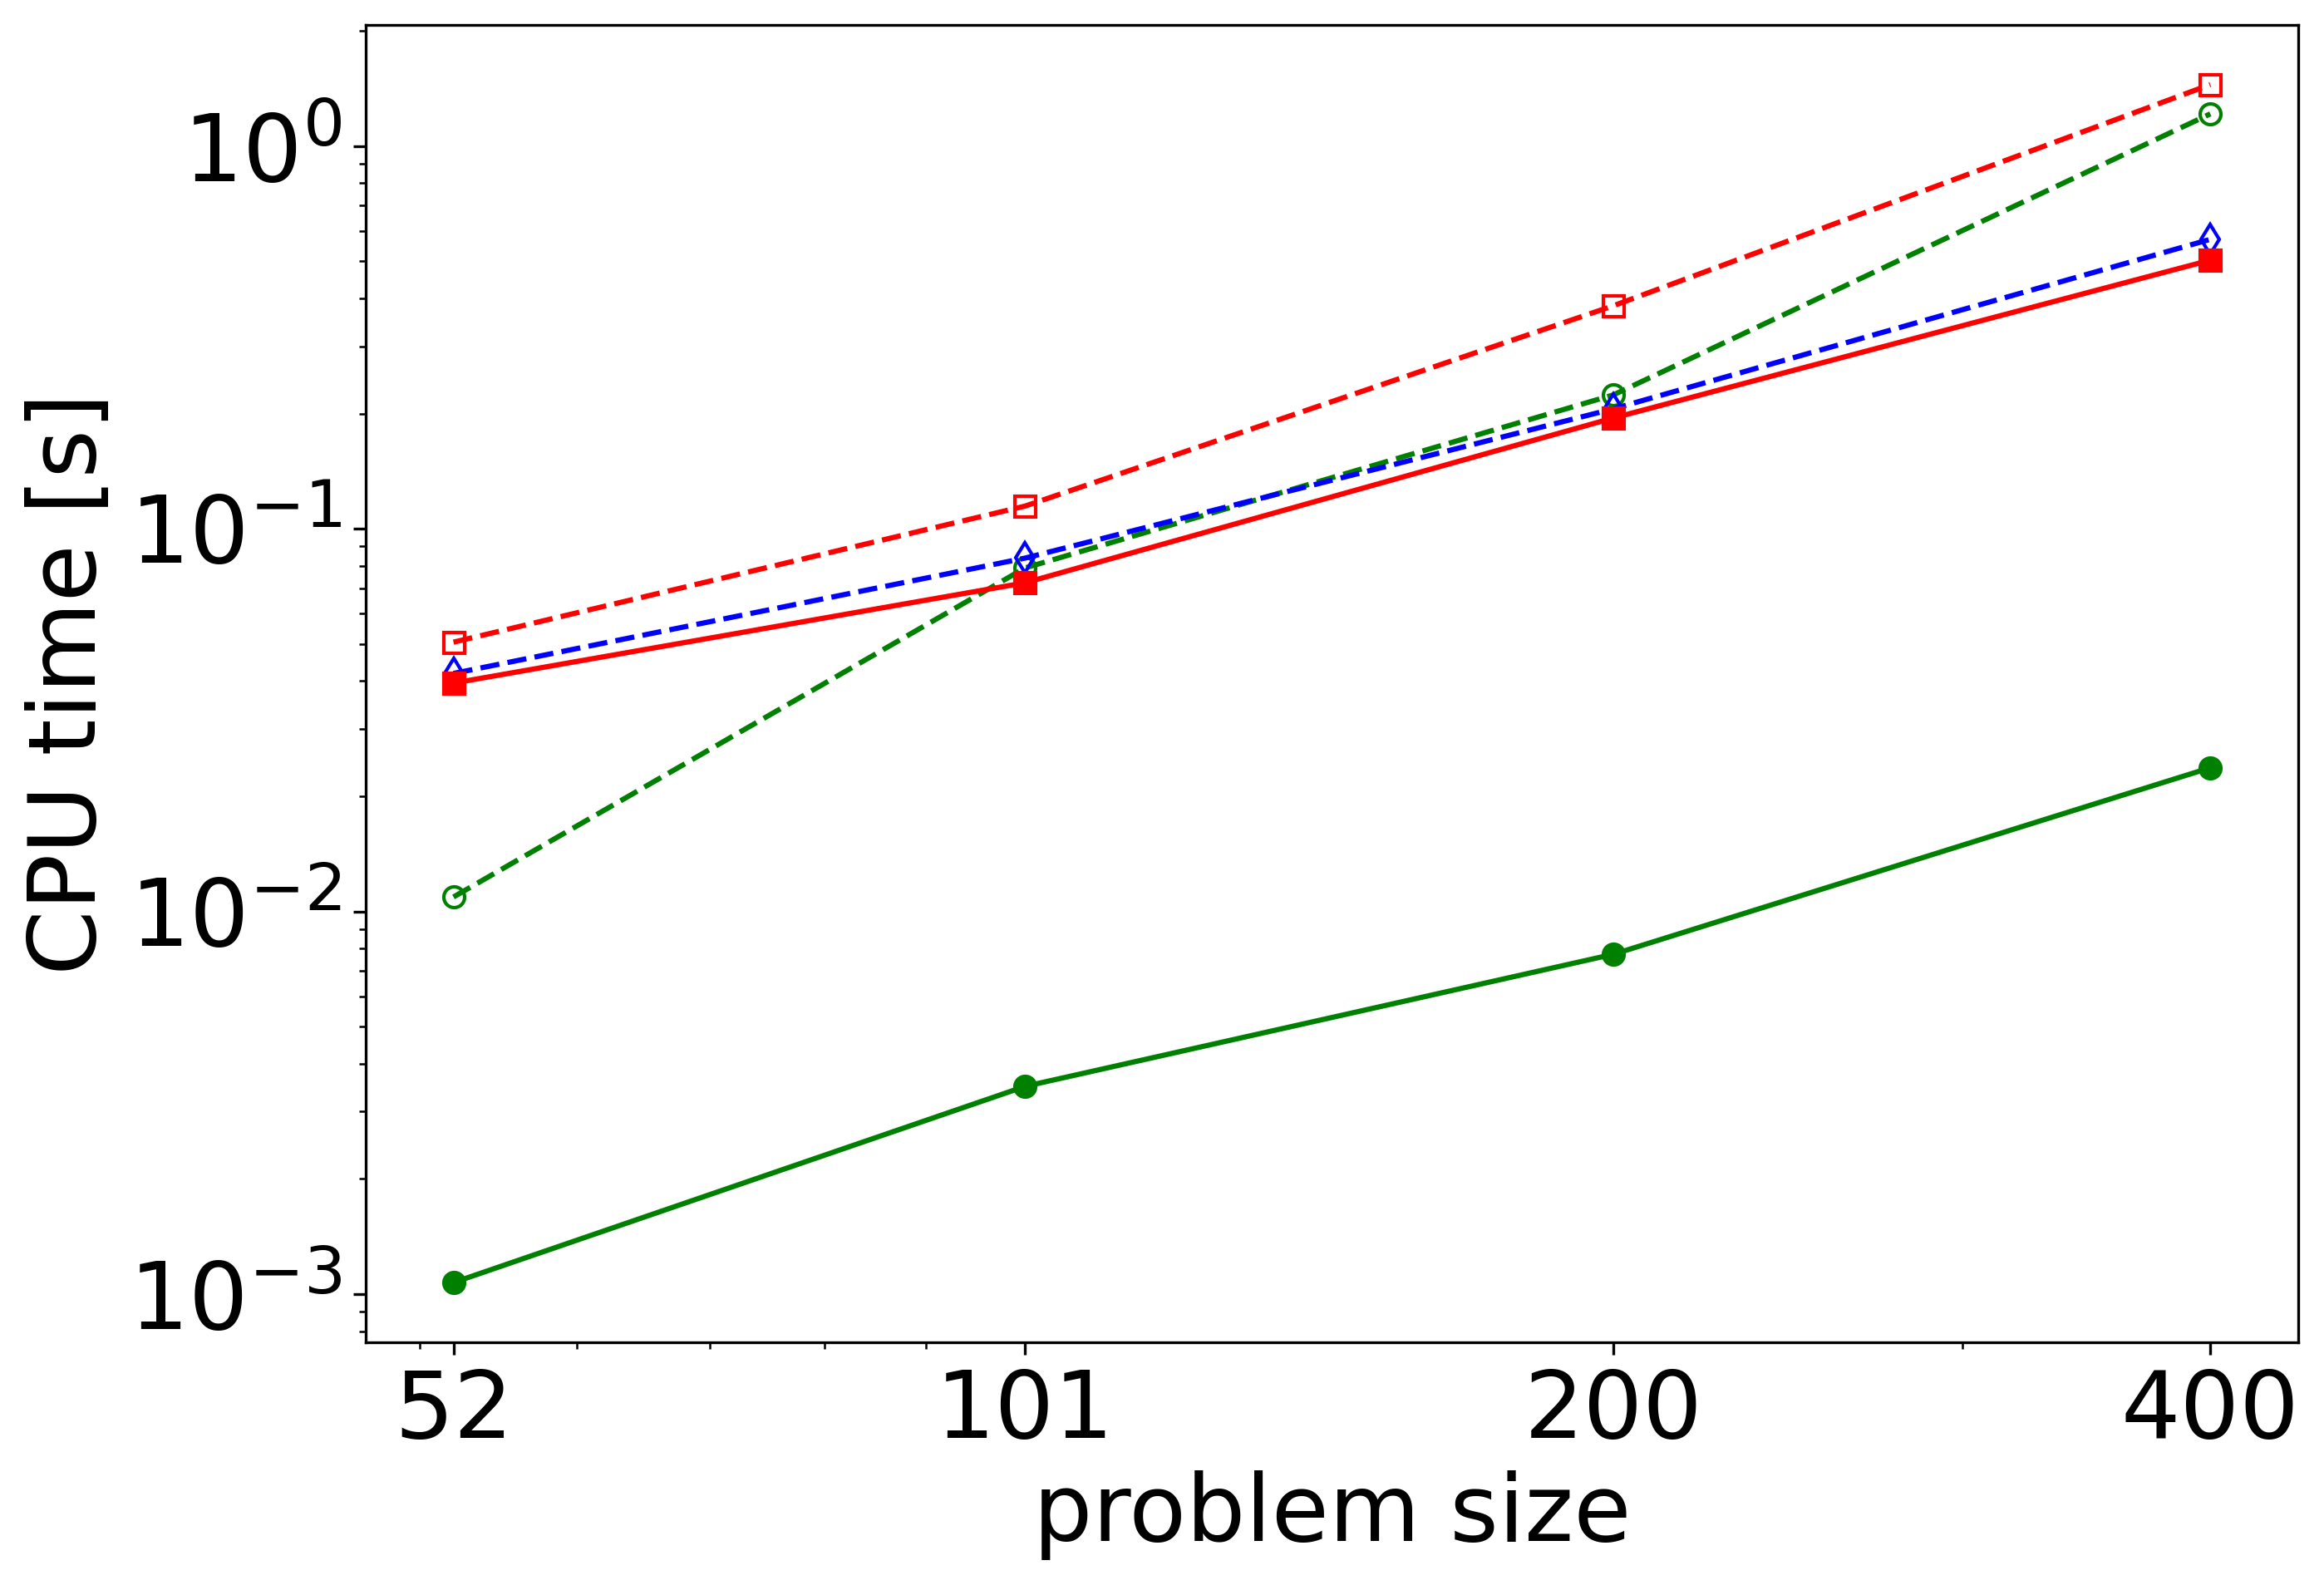
\includegraphics[width=1\textwidth]{images/TANDEM_TimePerRHSEvaluation_differentSizes.png}
		\subcaption{Average execution time of each RHS evaluation}
	\end{subfigure}
	\begin{subfigure}[b]{0.32\textwidth}
		\centering \hspace{-0.75cm}
		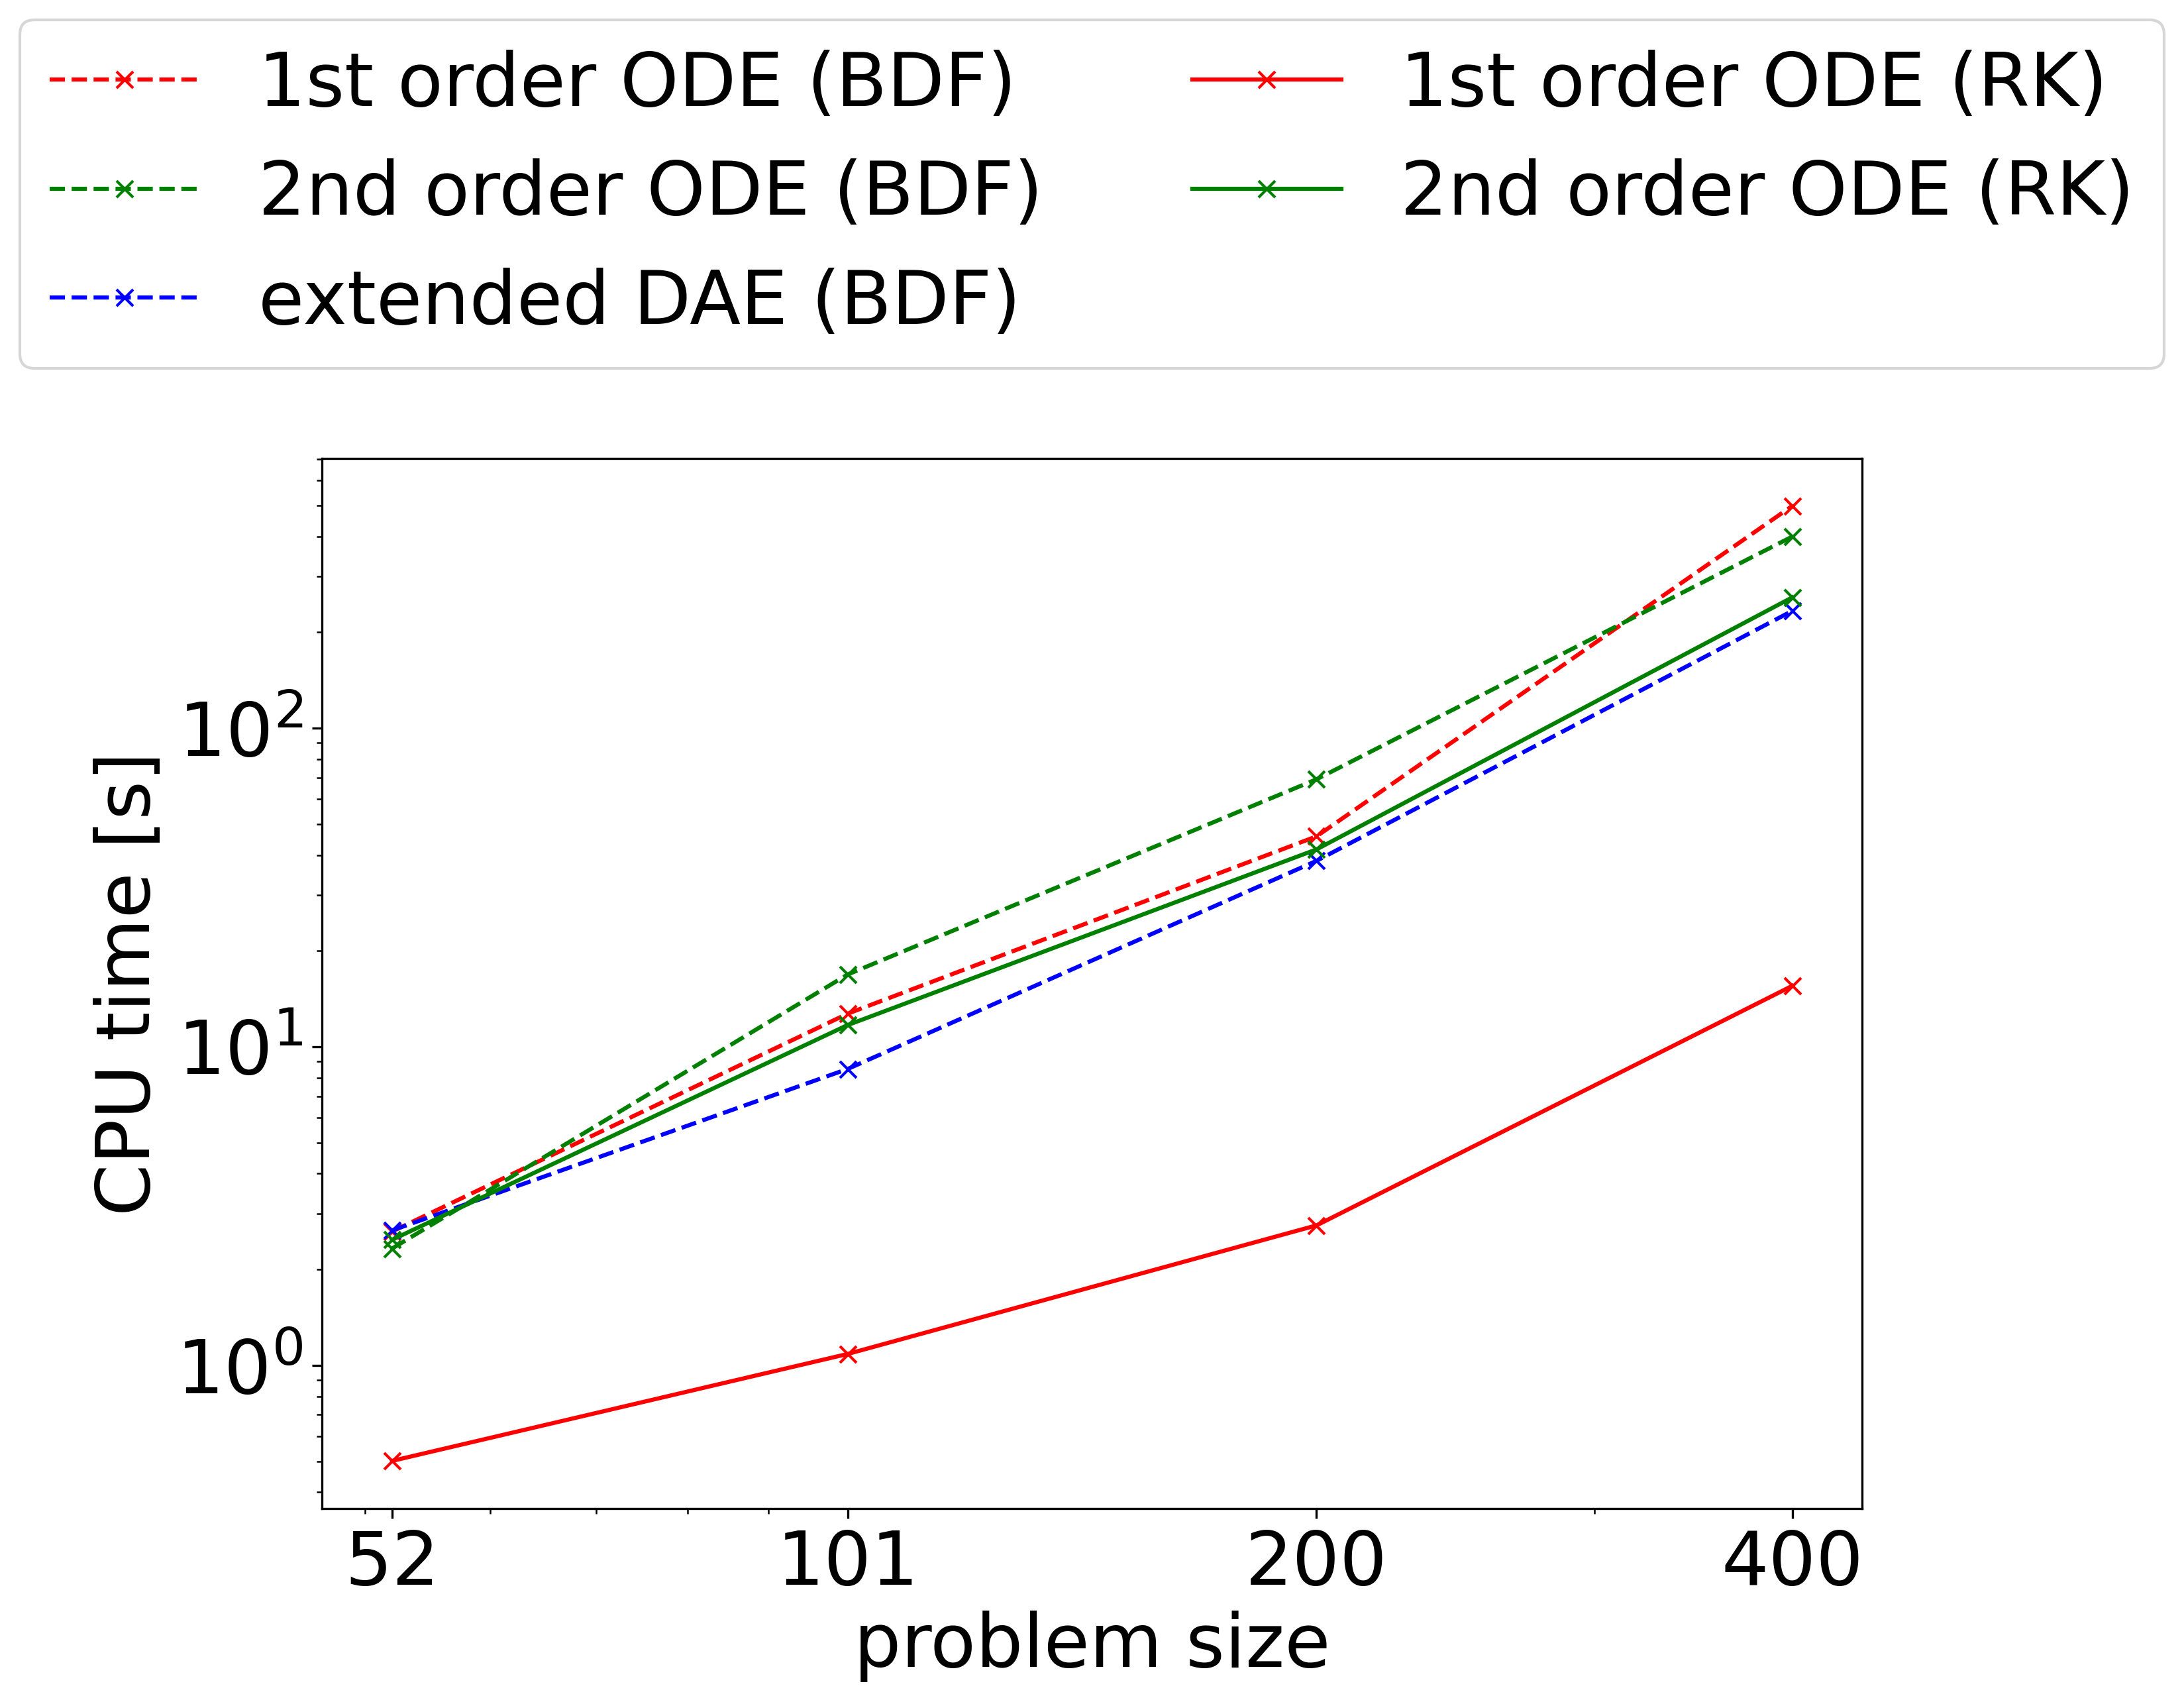
\includegraphics[width=1.18\textwidth]{images/TANDEM_CPU_Time_intialization.png}
		\subcaption{Execution time of the initialization phase} 
	\end{subfigure}
	\begin{subfigure}[b]{0.32\textwidth}
		\centering
		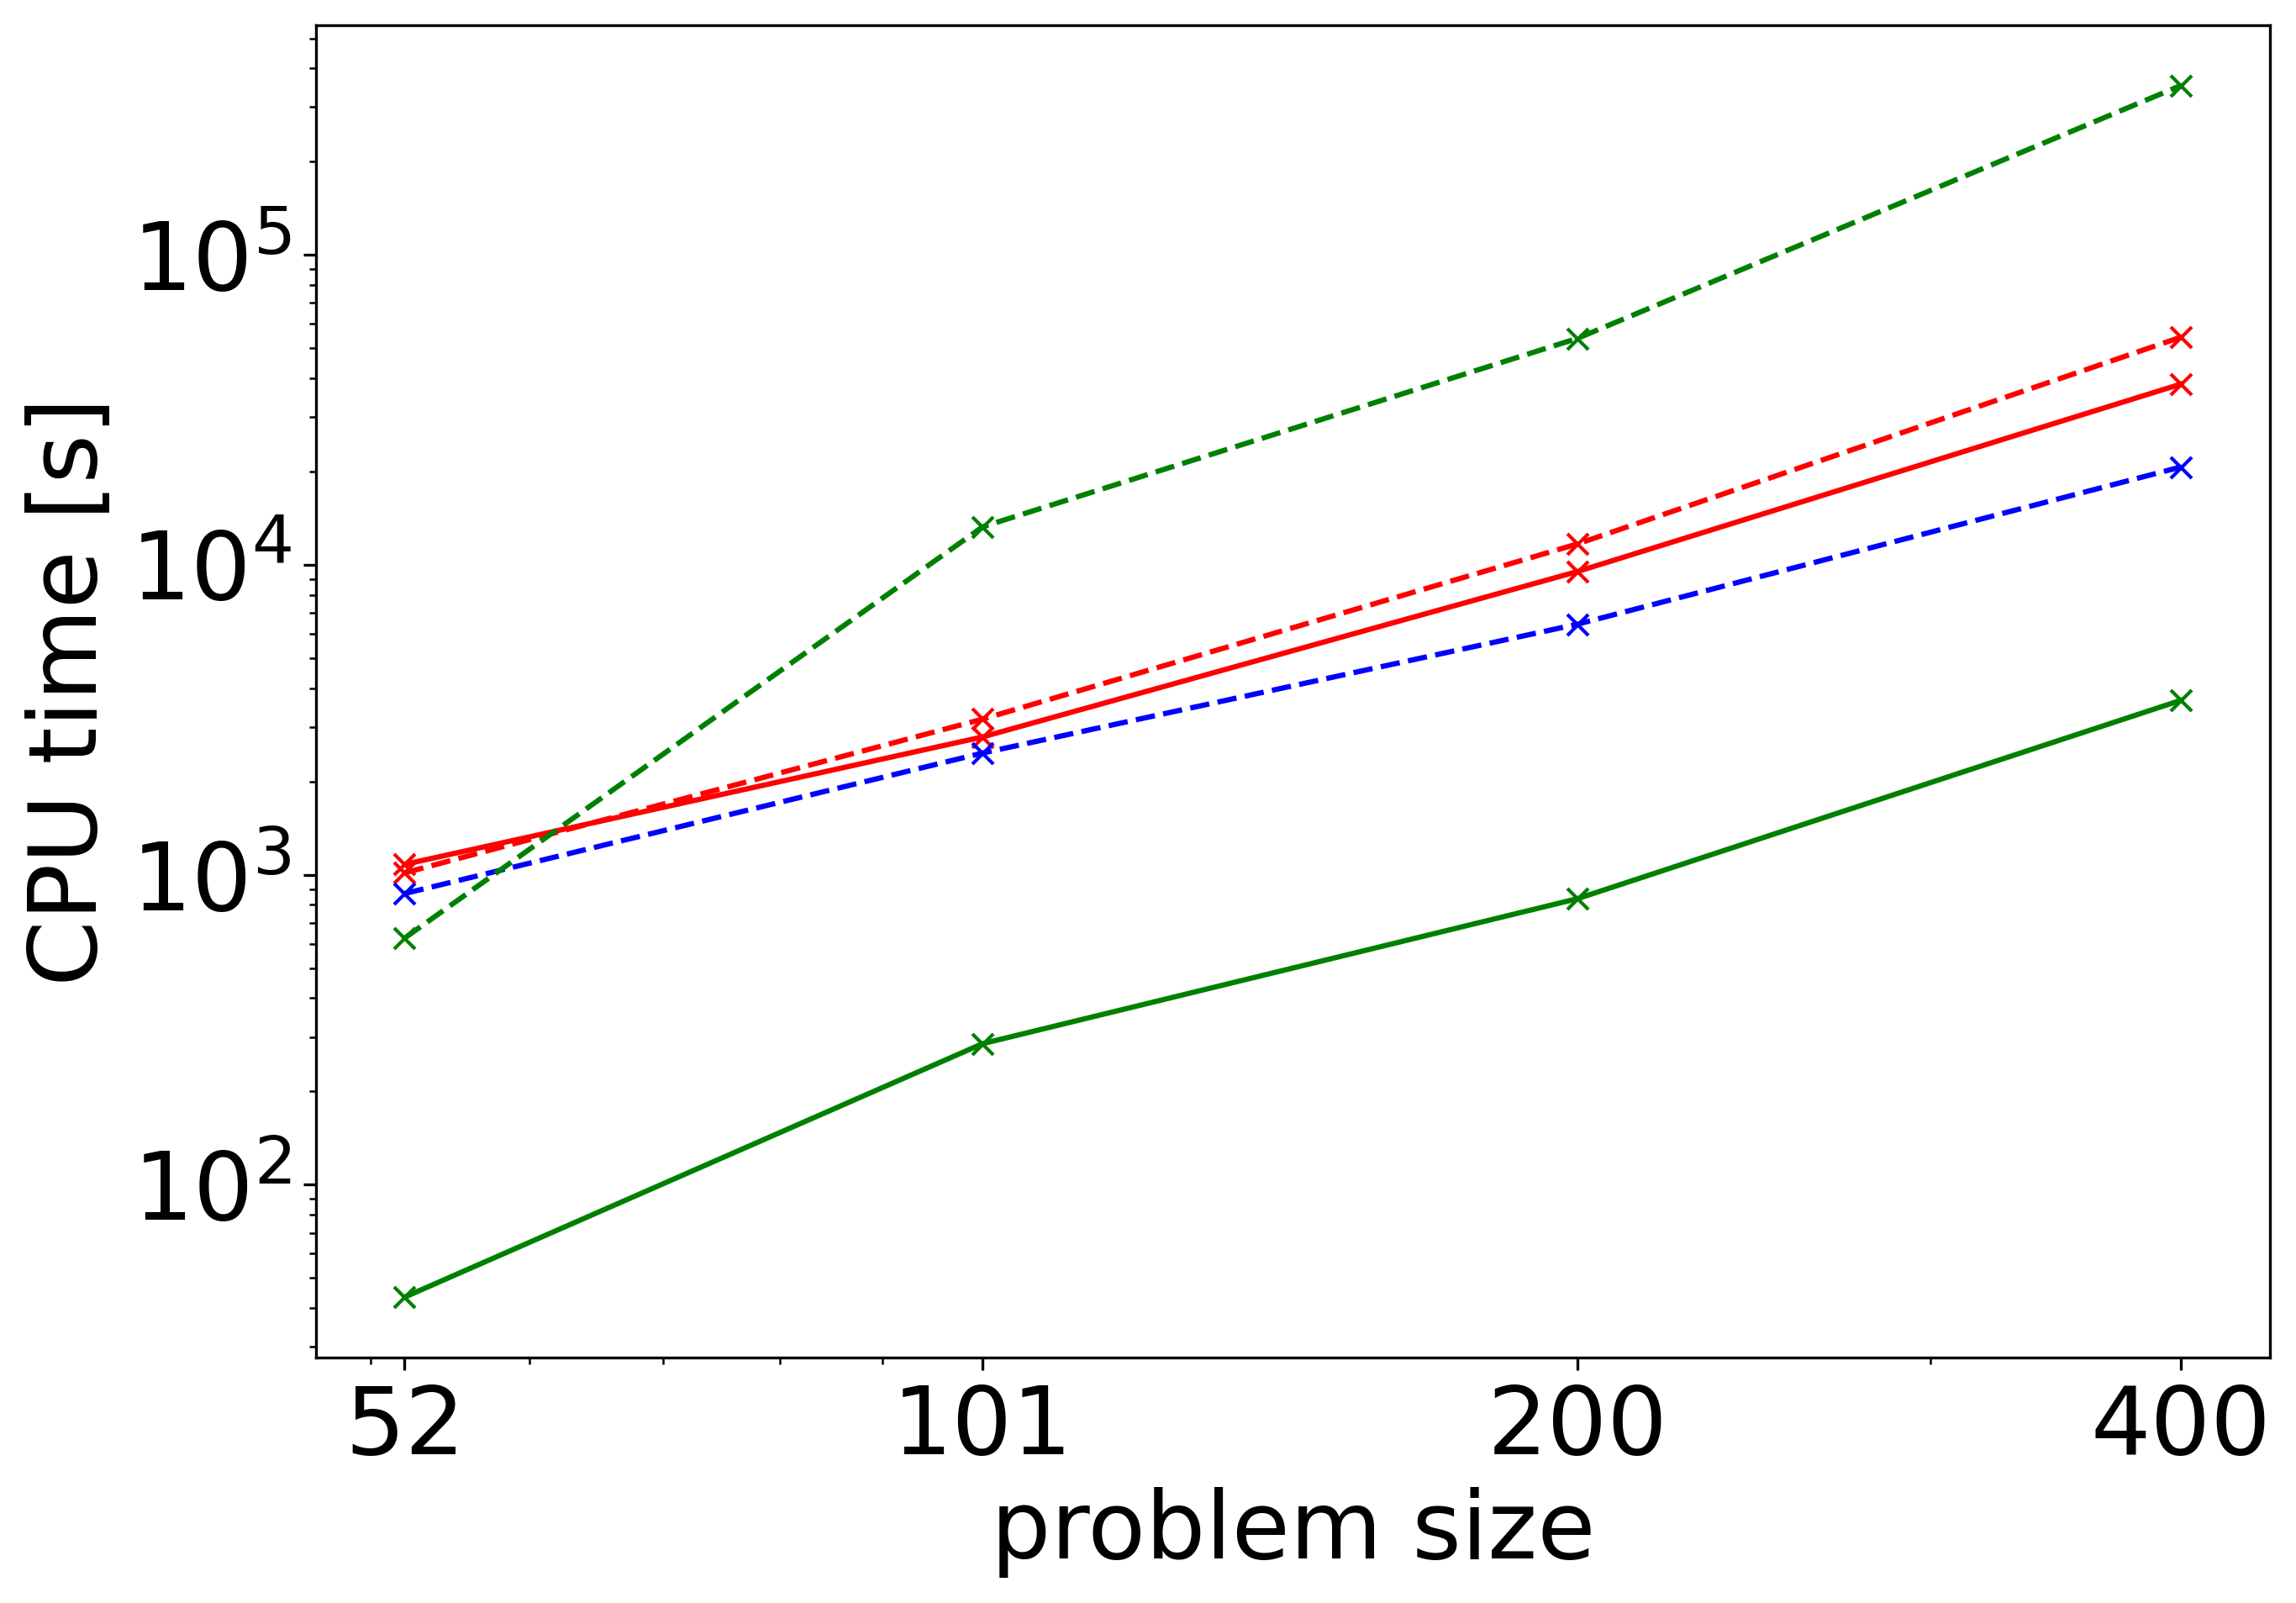
\includegraphics[width=1\textwidth]{images/TANDEM_CPU_Time_solving.png}
		\subcaption{Execution time of the solving phase\\ \ } 
	\end{subfigure}
	\caption{Execution time of different sections of the simulation with different problem sizes.}
	\label{fig:scalabilty_executionTimes}
\end{figure}

